% Customizable fields and text areas start with % >> below.
% Lines starting with the comment character (%) are normally removed before release outside the collaboration, but not those comments ending lines

% svn info. These are modified by svn at checkout time.
% The last version of these macros found before the maketitle will be the one on the front page,
% so only the main file is tracked.
% Do not edit by hand!
\RCS$Revision: 248542 $
\RCS$HeadURL: svn+ssh://svn.cern.ch/reps/tdr2/notes/DN-14-008/trunk/DN-14-008.tex $
\RCS$Id: DN-14-008.tex 248542 2014-06-27 14:15:24Z erdogan $
%%%%%%%%%%%%% local definitions %%%%%%%%%%%%%%%%%%%%%
% This allows for switching between one column and two column (cms@external) layouts
% The widths should  be modified for your particular figures. You'll need additional copies if you have more than one standard figure size.
\newlength\cmsFigWidth
\ifthenelse{\boolean{cms@external}}{\setlength\cmsFigWidth{0.85\columnwidth}}{\setlength\cmsFigWidth{0.4\textwidth}}
\ifthenelse{\boolean{cms@external}}{\providecommand{\cmsLeft}{top}}{\providecommand{\cmsLeft}{left}}
\ifthenelse{\boolean{cms@external}}{\providecommand{\cmsRight}{bottom}}{\providecommand{\cmsRight}{right}}
%%%%%%%%%%%%%%%  Title page %%%%%%%%%%%%%%%%%%%%%%%%
\cmsNoteHeader{DN-14-008} % This is over-written in the CMS environment: useful as preprint no. for export versions
% >> Title: please make sure that the non-TeX equivalent is in PDFTitle below
\title{A new trigger concept for muons in the barrel region of the CMS experiment: Muon Track fast Tag}

% >> Authors
%Author is always "The CMS Collaboration" for PAS and papers, so author, etc, below will be ignored in those cases
%For multiple affiliations, create an address entry for the combination
%To mark authors as primary, use the \author* form
\address[neu]{RWTH Aachen University}
\author[neu]{Yusuf Erdogan}
\author[neu]{G\"unter Fl\"ugge}
\author[neu]{Thomas Hebbeker}
\author[neu]{Andreas K\"unsken}
\author[neu]{Erik Dietz-Laursson}
\author[neu]{Markus Merschmeyer}
\author[neu]{Oliver Pooth}
\author[neu]{Thomas Radermacher}
\author[neu]{Florian Scheuch}
\author[neu]{Achim Stahl}
\author[neu]{Simon Weingarten}
\author[neu]{Lars Weinstock}

% >> Date
% The date is in yyyy/mm/dd format. Today has been
% redefined to match, but if the date needs to be fixed, please write it in this fashion.
% For papers and PAS, \today is taken as the date the head file (this one) was last modified according to svn: see the RCS Id string above.
% For the final version it is best to "touch" the head file to make sure it has the latest date.
\date{\today}

% >> Abstract
% Abstract processing:
% 1. **DO NOT use \include or \input** to include the abstract: our abstract extractor will not search through other files than this one.
% 2. **DO NOT use %**                  to comment out sections of the abstract: the extractor will still grab those lines (and they won't be comments any longer!).
% 3. For PASs: **DO NOT use tex macros**         in the abstract: CDS MathJax processor used on the abstract doesn't understand them _and_ will only look within $$. The abstracts for papers are hand formatted so macros are okay.
\abstract{
Triggering on high $p_t$ muons at the projected high luminosity LHC (HL-LHC) with an expected instantaneous luminosity of $10^{35}/(\mathrm{cm}^2 \cdot\mathrm{s})$ will be 
one major challenge for the CMS experiment from 2023 on. With the {\bf M}uon  {\bf T}rack fast {\bf T}ag (MTT) a new detector subsystem is proposed that can help to keep the 
Level-1 trigger rate low enough without increasing the $p_t$ thresholds for single muons. The trigger concept must be extended by combining the information of the inner tracking
system with a fast muon tag which is also able to reduce the problem with ambiguities of simultaneously traversing muons leading to so-called ghost hits in the muon systems.
}

% >> PDF Metadata
% Do not comment out the following hypersetup lines (metadata). They will disappear in NODRAFT mode and are needed by CDS.
% Also: make sure that the values of the metadata items are sensible and are in plain text:
% (1) no TeX! -- for \sqrt{s} use sqrt(s) -- this will show with extra quote marks in the draft version but is okay).
% (2) no %.
% (3) No curly braces {}.
\hypersetup{%
pdfauthor={George Alverson, Lucas Taylor, A. Cern Person},%
pdftitle={A new trigger concept for muons in the barrel region of the CMS experiment: Muon Track fast Tag},%
pdfsubject={CMS},%
pdfkeywords={CMS, physics, software, computing}}

\maketitle %maketitle comes after all the front information has been supplied
% >> Text
%%%%%%%%%%%%%%%%%%%%%%%%%%%%%%%%  Begin text %%%%%%%%%%%%%%%%%%%%%%%%%%%%%
%% **DO NOT REMOVE THE BIBLIOGRAPHY** which is located before the appendix.
%% You can take the text between here and the bibiliography as an example which you should replace with the actual text of your document.
%% If you include other TeX files, be sure to use "\input{filename}" rather than "\input filename".
%% The latter works for you, but our parser looks for the braces and will break when uploading the document.
%%%%%%%%%%%%%%%

\section{Abstract}
Triggering on high $p_t$ muons at the projected high luminosity LHC (HL-LHC) with an expected instantaneous luminosity of $10^{35}/(\mathrm{cm}^2 \cdot\mathrm{s})$ will be 
one of the major challenges for the CMS experiment. With the {\bf M}uon  {\bf T}rack fast {\bf T}ag (MTT) a new detector subsystem is proposed that can help to keep the 
Level-1 trigger rate low enough without increasing the $p_t$ thresholds for single muons. The trigger concept must be extended by combining the information of the inner tracking
system with a fast muon tag which is also able to reduce the problem with ambiguities of simultaneously traversing muons leading to so-called ghost hits in the muon systems. 

\section{Motivation for a Muon Track fast Tag (MTT) at CMS}

As of 2023 the CMS experiment at the LHC is expected to operate at the high luminosity LHC (HL-LHC). Up to 1000~fb$^{-1}$ of data will be collected per year with an 
instantaneous luminosity that will be increased by a factor of ten compared to the running LHC with a design luminosity of $10^{34}/(\mathrm{cm}^2 \cdot\mathrm{s})$. New physics 
scenarios and extended limits which are expected and hoped for in the coming years are displayed in Figure~\ref{fig:schedule_concept} where the integrated luminosity is shown versus 
time. 
\begin{figure}[htbp]
\centering
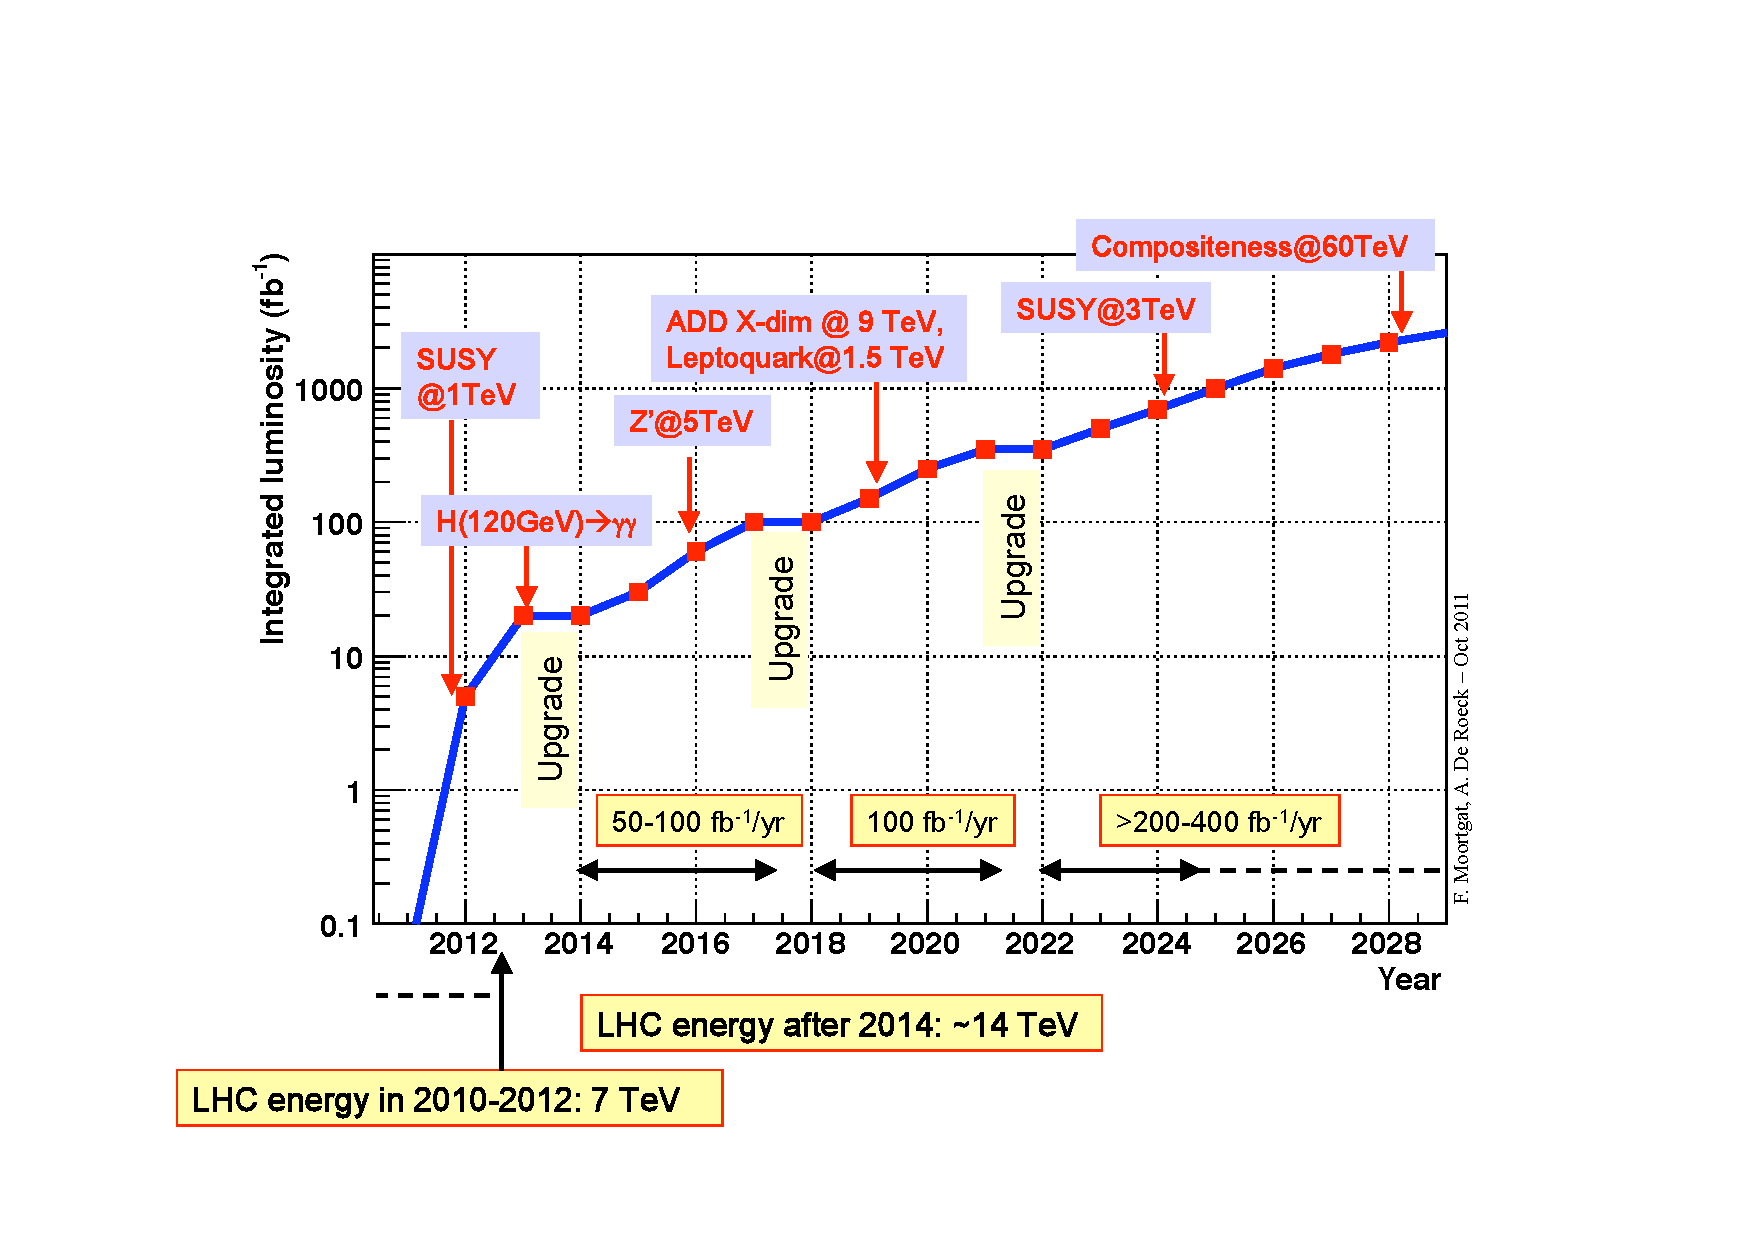
\includegraphics[width=0.45\textwidth]{Figures/pooth/schedule.pdf}
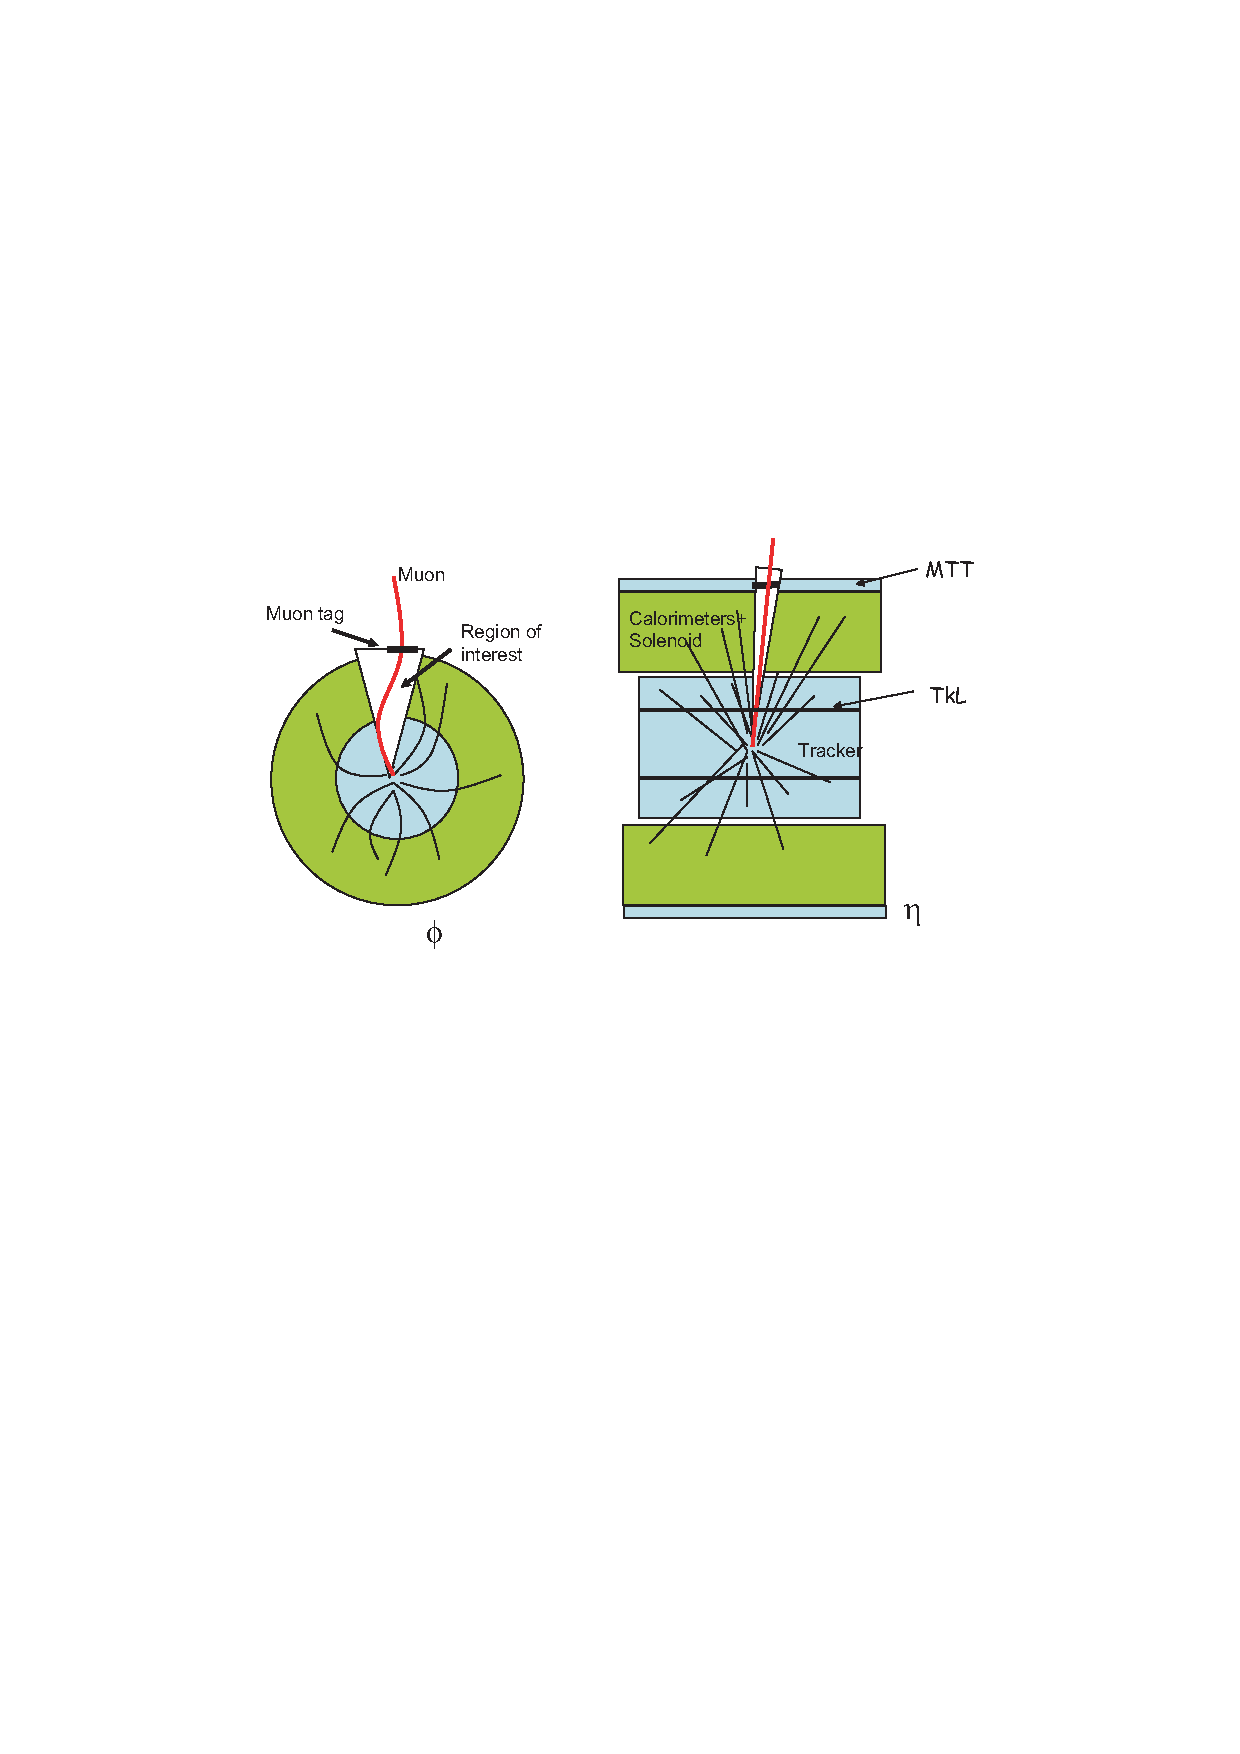
\includegraphics[width=0.52\textwidth]{Figures/pooth/mtt_concept_a.pdf}
\caption{Left: The integrated luminosity versus time for the periods before, between and after the three long shutdowns to come~\cite{schedule}. Right: The Muon Track fast Tag concept~\cite{mtt_concept}. } 
\label{fig:schedule_concept}
\end{figure}
Various scenarios are under discussion to increase the amount of data to search for events with extremely small cross sections, e.g. increasing beam energy, higher bunch 
crossing frequency and higher number of protons per bunch. The CMS roadmap for the future long shutdowns is shown in Figure~\ref{fig:upgrade_planning}.
\begin{figure}[htbp]
\centering
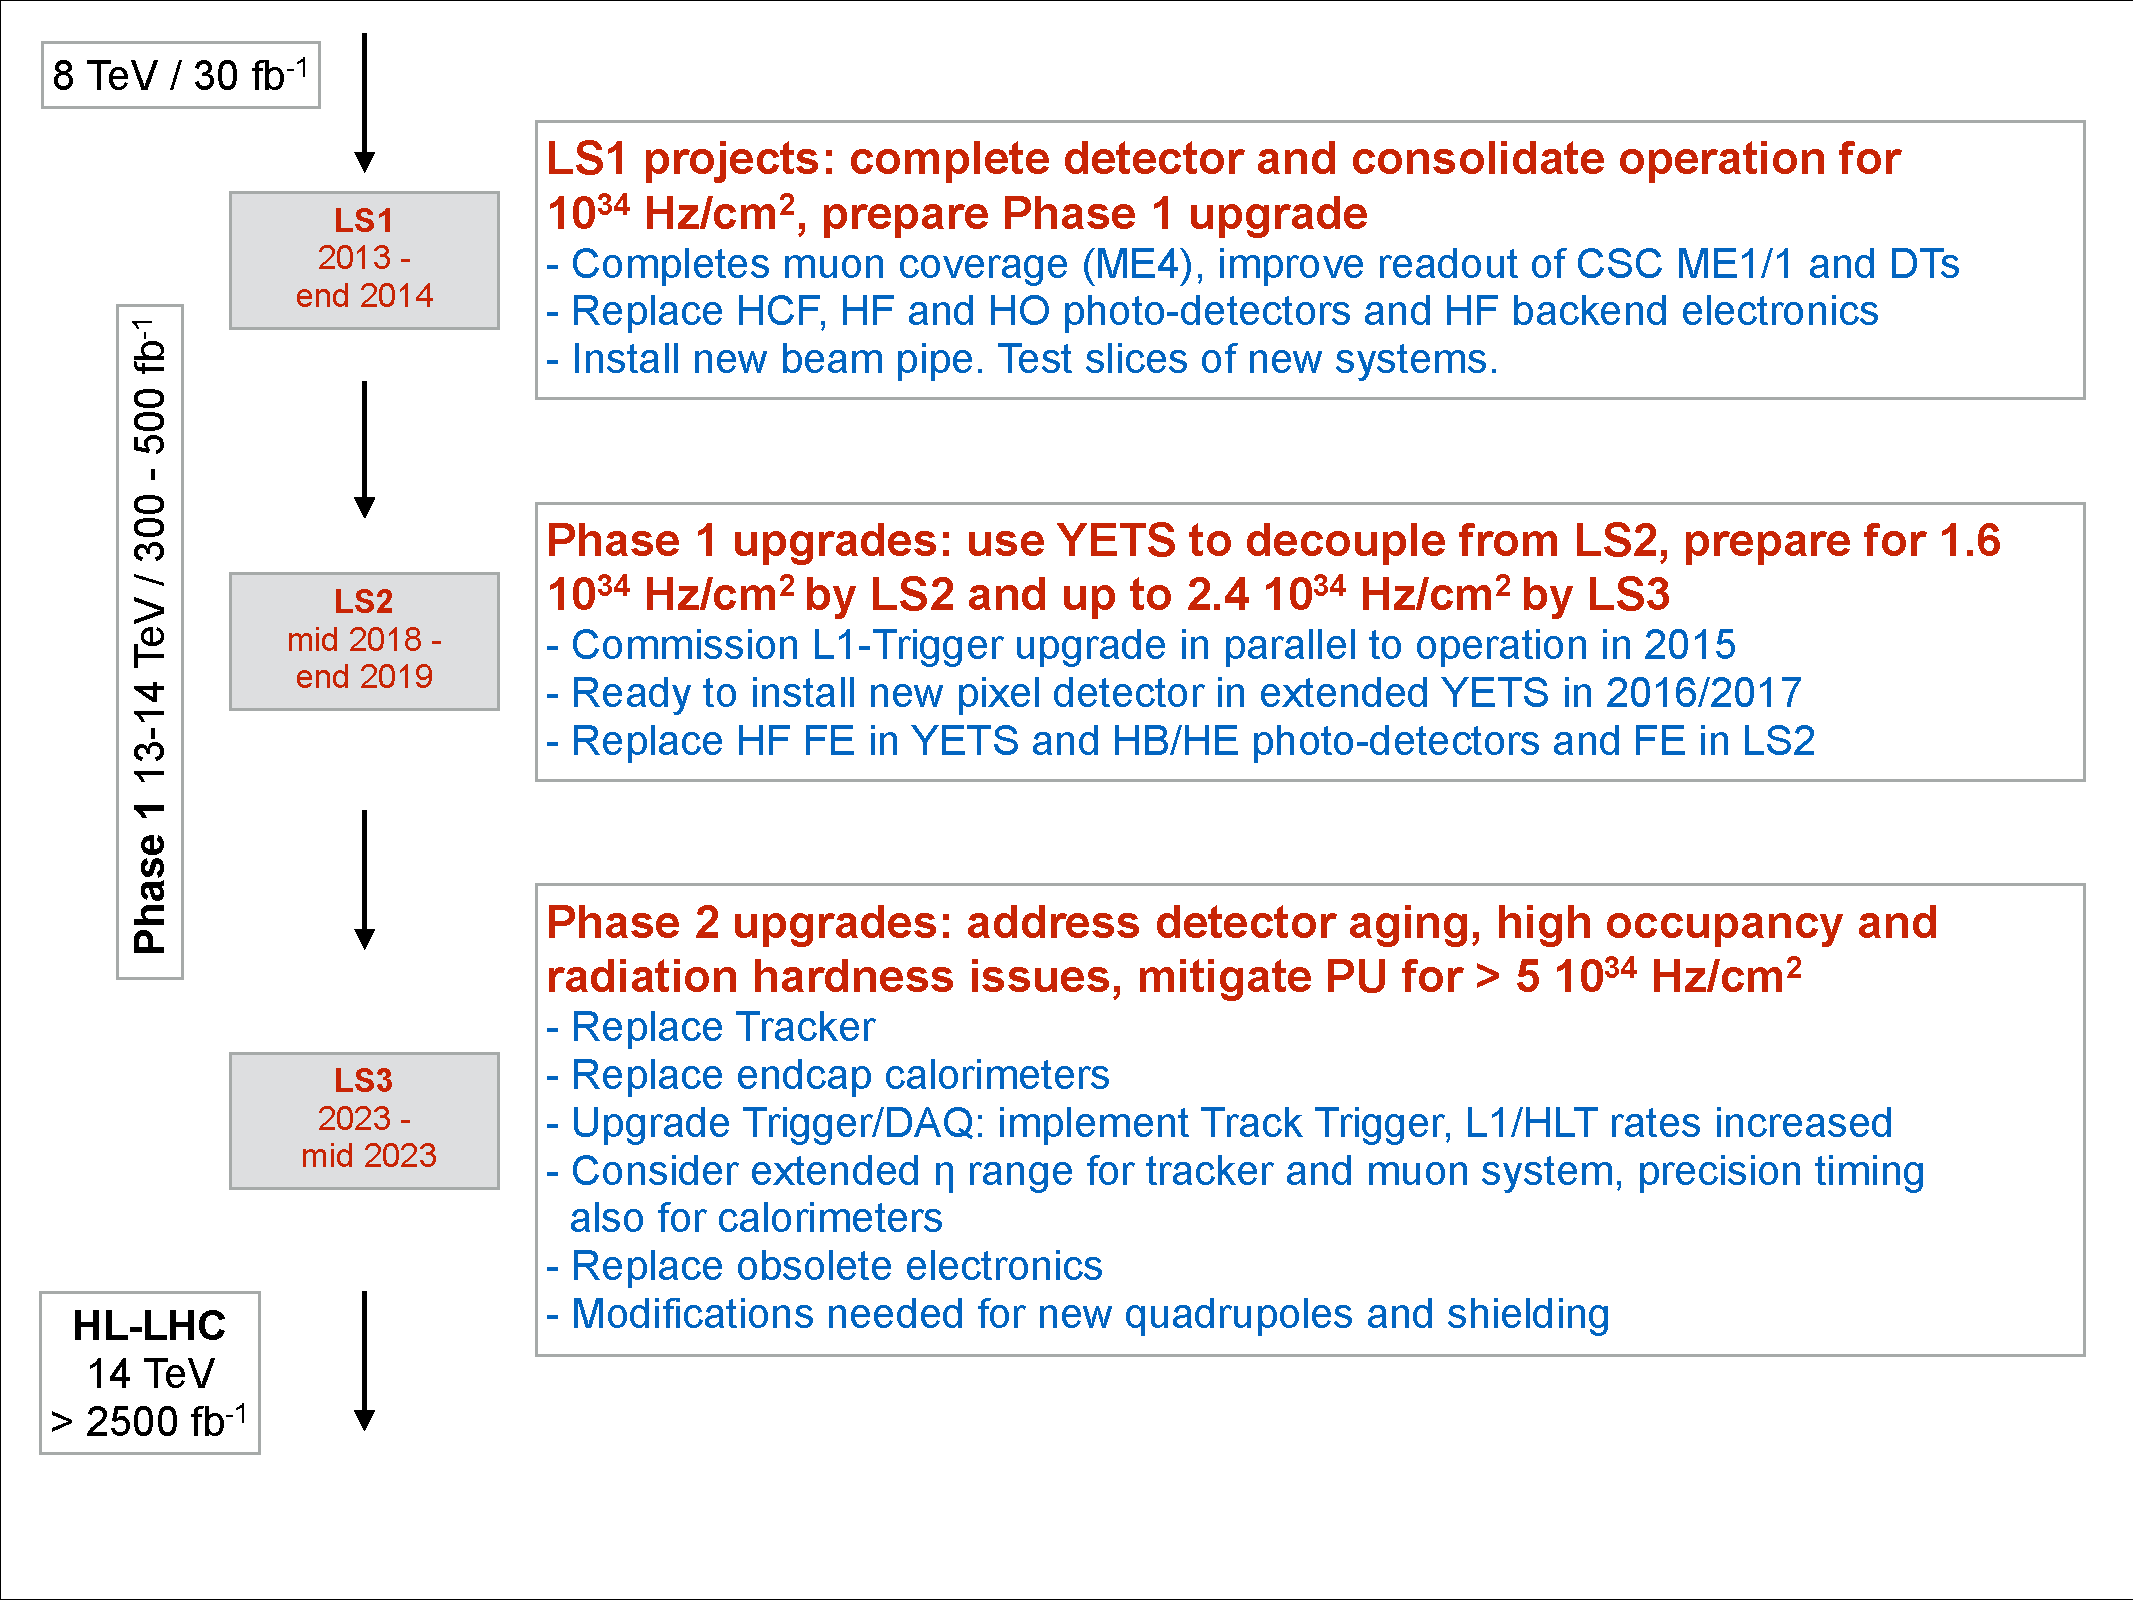
\includegraphics[width=0.8\textwidth]{Figures/pooth/upgrade_planning.pdf}\\
\caption{Upgrade planning~\cite{upgrade_planning}.} 
\label{fig:upgrade_planning}
\end{figure}

To trigger on high $p_t$ muons at $10^{35}/(\mathrm{cm}^2 \cdot\mathrm{s})$ while keeping the Level-1 trigger rate low the trigger concept needs to be extended. With the MTT (see 
Figure~\ref{fig:schedule_concept}, right), a fast 2D trigger system located between the CMS solenoid and the inner muon stations is proposed in~\cite{mtt_concept} to cope with high 
muon rates without increasing the $p_t$ thresholds. Just increasing the thresholds would be an inefficient way as shown in Figure~\ref{fig:pt_threshold}, mainly due to poorly 
reconstructed muon $p_t$ on Level-1. 
\begin{figure}[htbp]
\centering
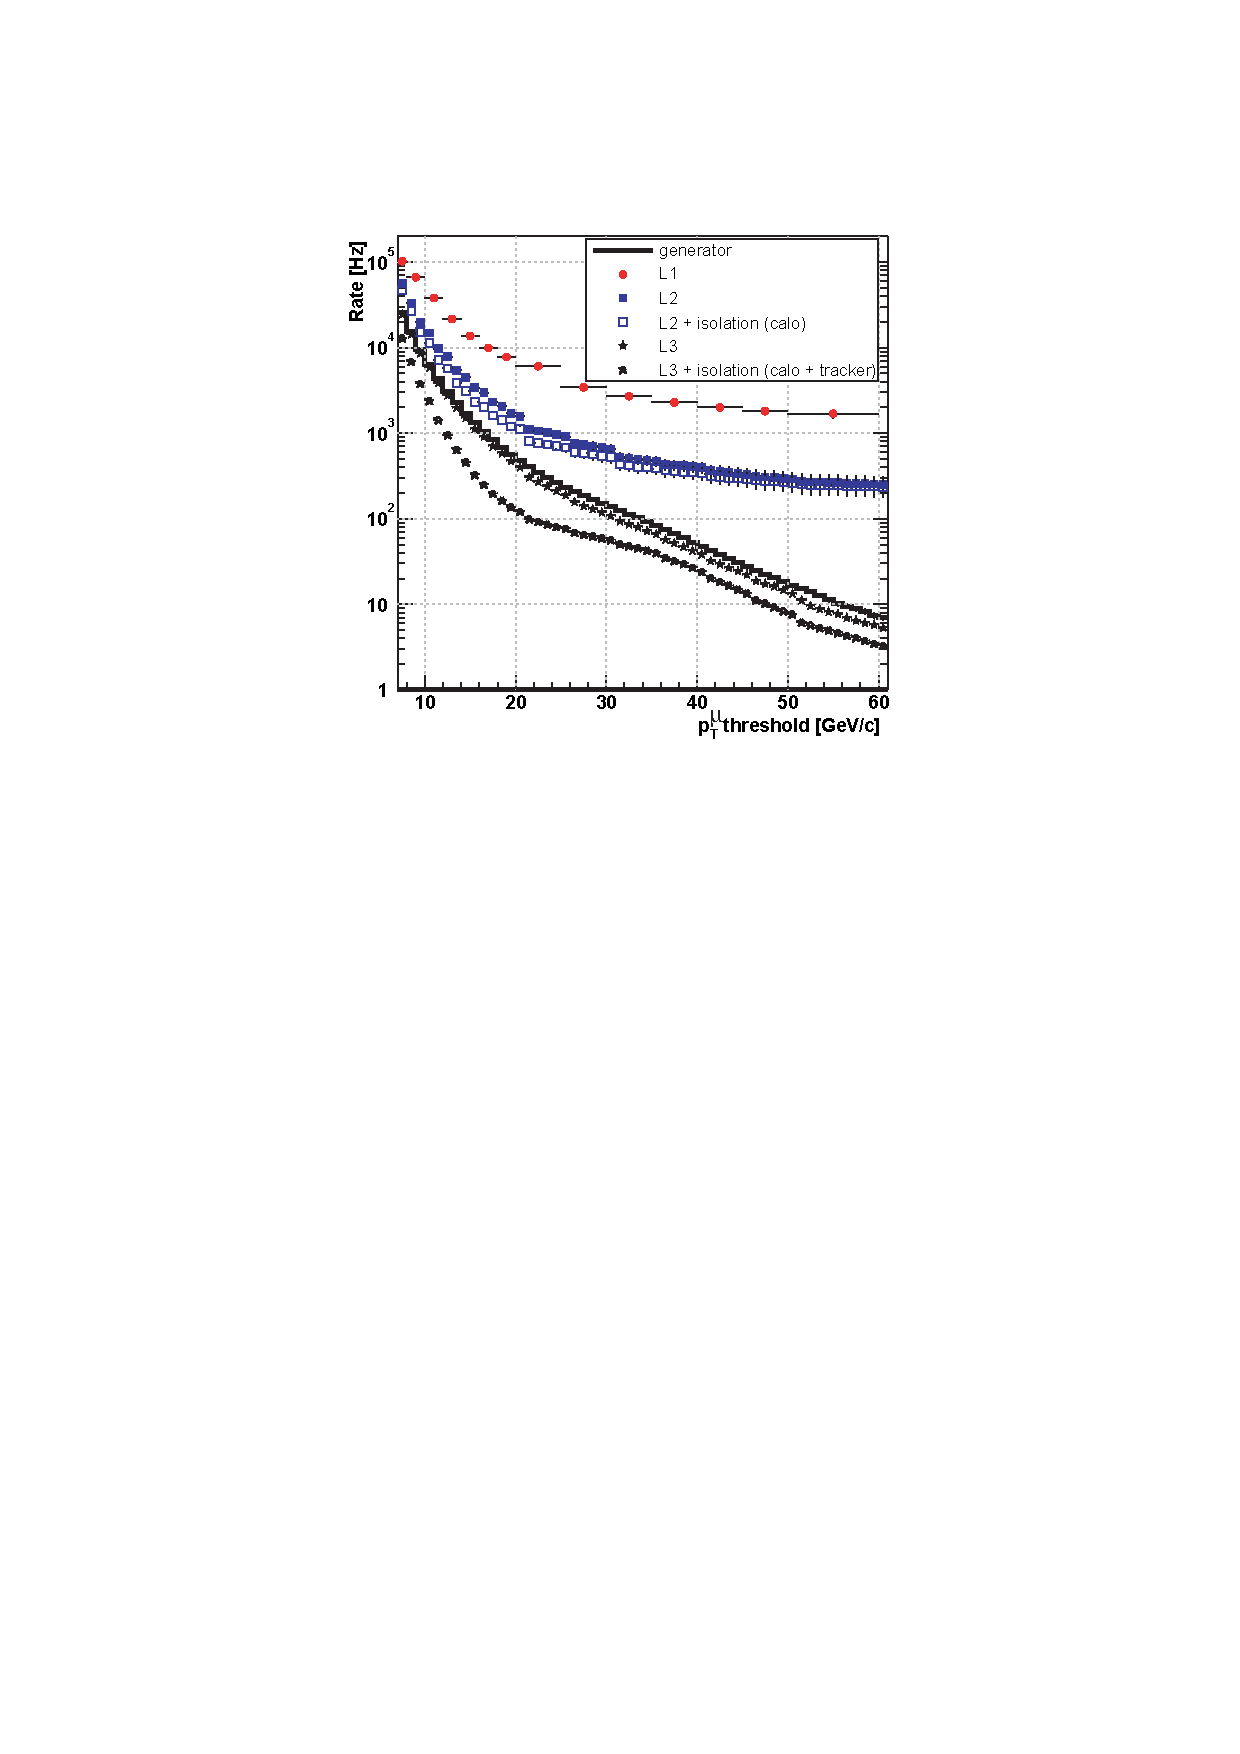
\includegraphics[width=0.5\textwidth]{Figures/pooth/pt_threshold.pdf}
\caption{Rates for different trigger levels as a function of the muon $p_t$ threshold~\cite{pt_threshold}.}
\label{fig:pt_threshold}
\end{figure}

Tiles of fast plastic scintillator material read out by silicon photomultipliers (SiPMs) are under investigation to provide the additional detector layer in the very limited space available 
between the CMS solenoid and the first muon stations~\cite{dn2014-020}. The existing outer layers of the Hadron Calorimeter (HO)  can serve as a perfect testbed for these studies. In the barrel region the 
SiPM signals of the outer layers of the Hadron Outer Calorimeter could be used in the muon trigger at Level-1. The benefits of this layer for MIP identification, punch through rejection 
and resolution of ambiguities in the DT system are described in this note. For Run II a trigger link has been established that makes the HO signals available for building Level-1 muon 
trigger primitives together with inputs from DT and RPC. Based on these data, an optimization of the HO granularity for Level-1 muon triggering purposes in Phase-2 can be envisaged. 

By combining the information from various subsystems the muon momentum resolution can be improved in the Level-1 trigger system. The inner silicon based tracking system provides 
an excellent $p_t$ measurement and with the MTT it is possible to tag regions of interest in case of high $p_t$ muons. In addition the MTT can resolve possible muon 
ambiguities at very high luminosities (ghost rejection). A measured ghost and a possible solution to resolve it are shown in Figure~\ref{fig:ghosts}.
\begin{figure}[htbp]
\centering
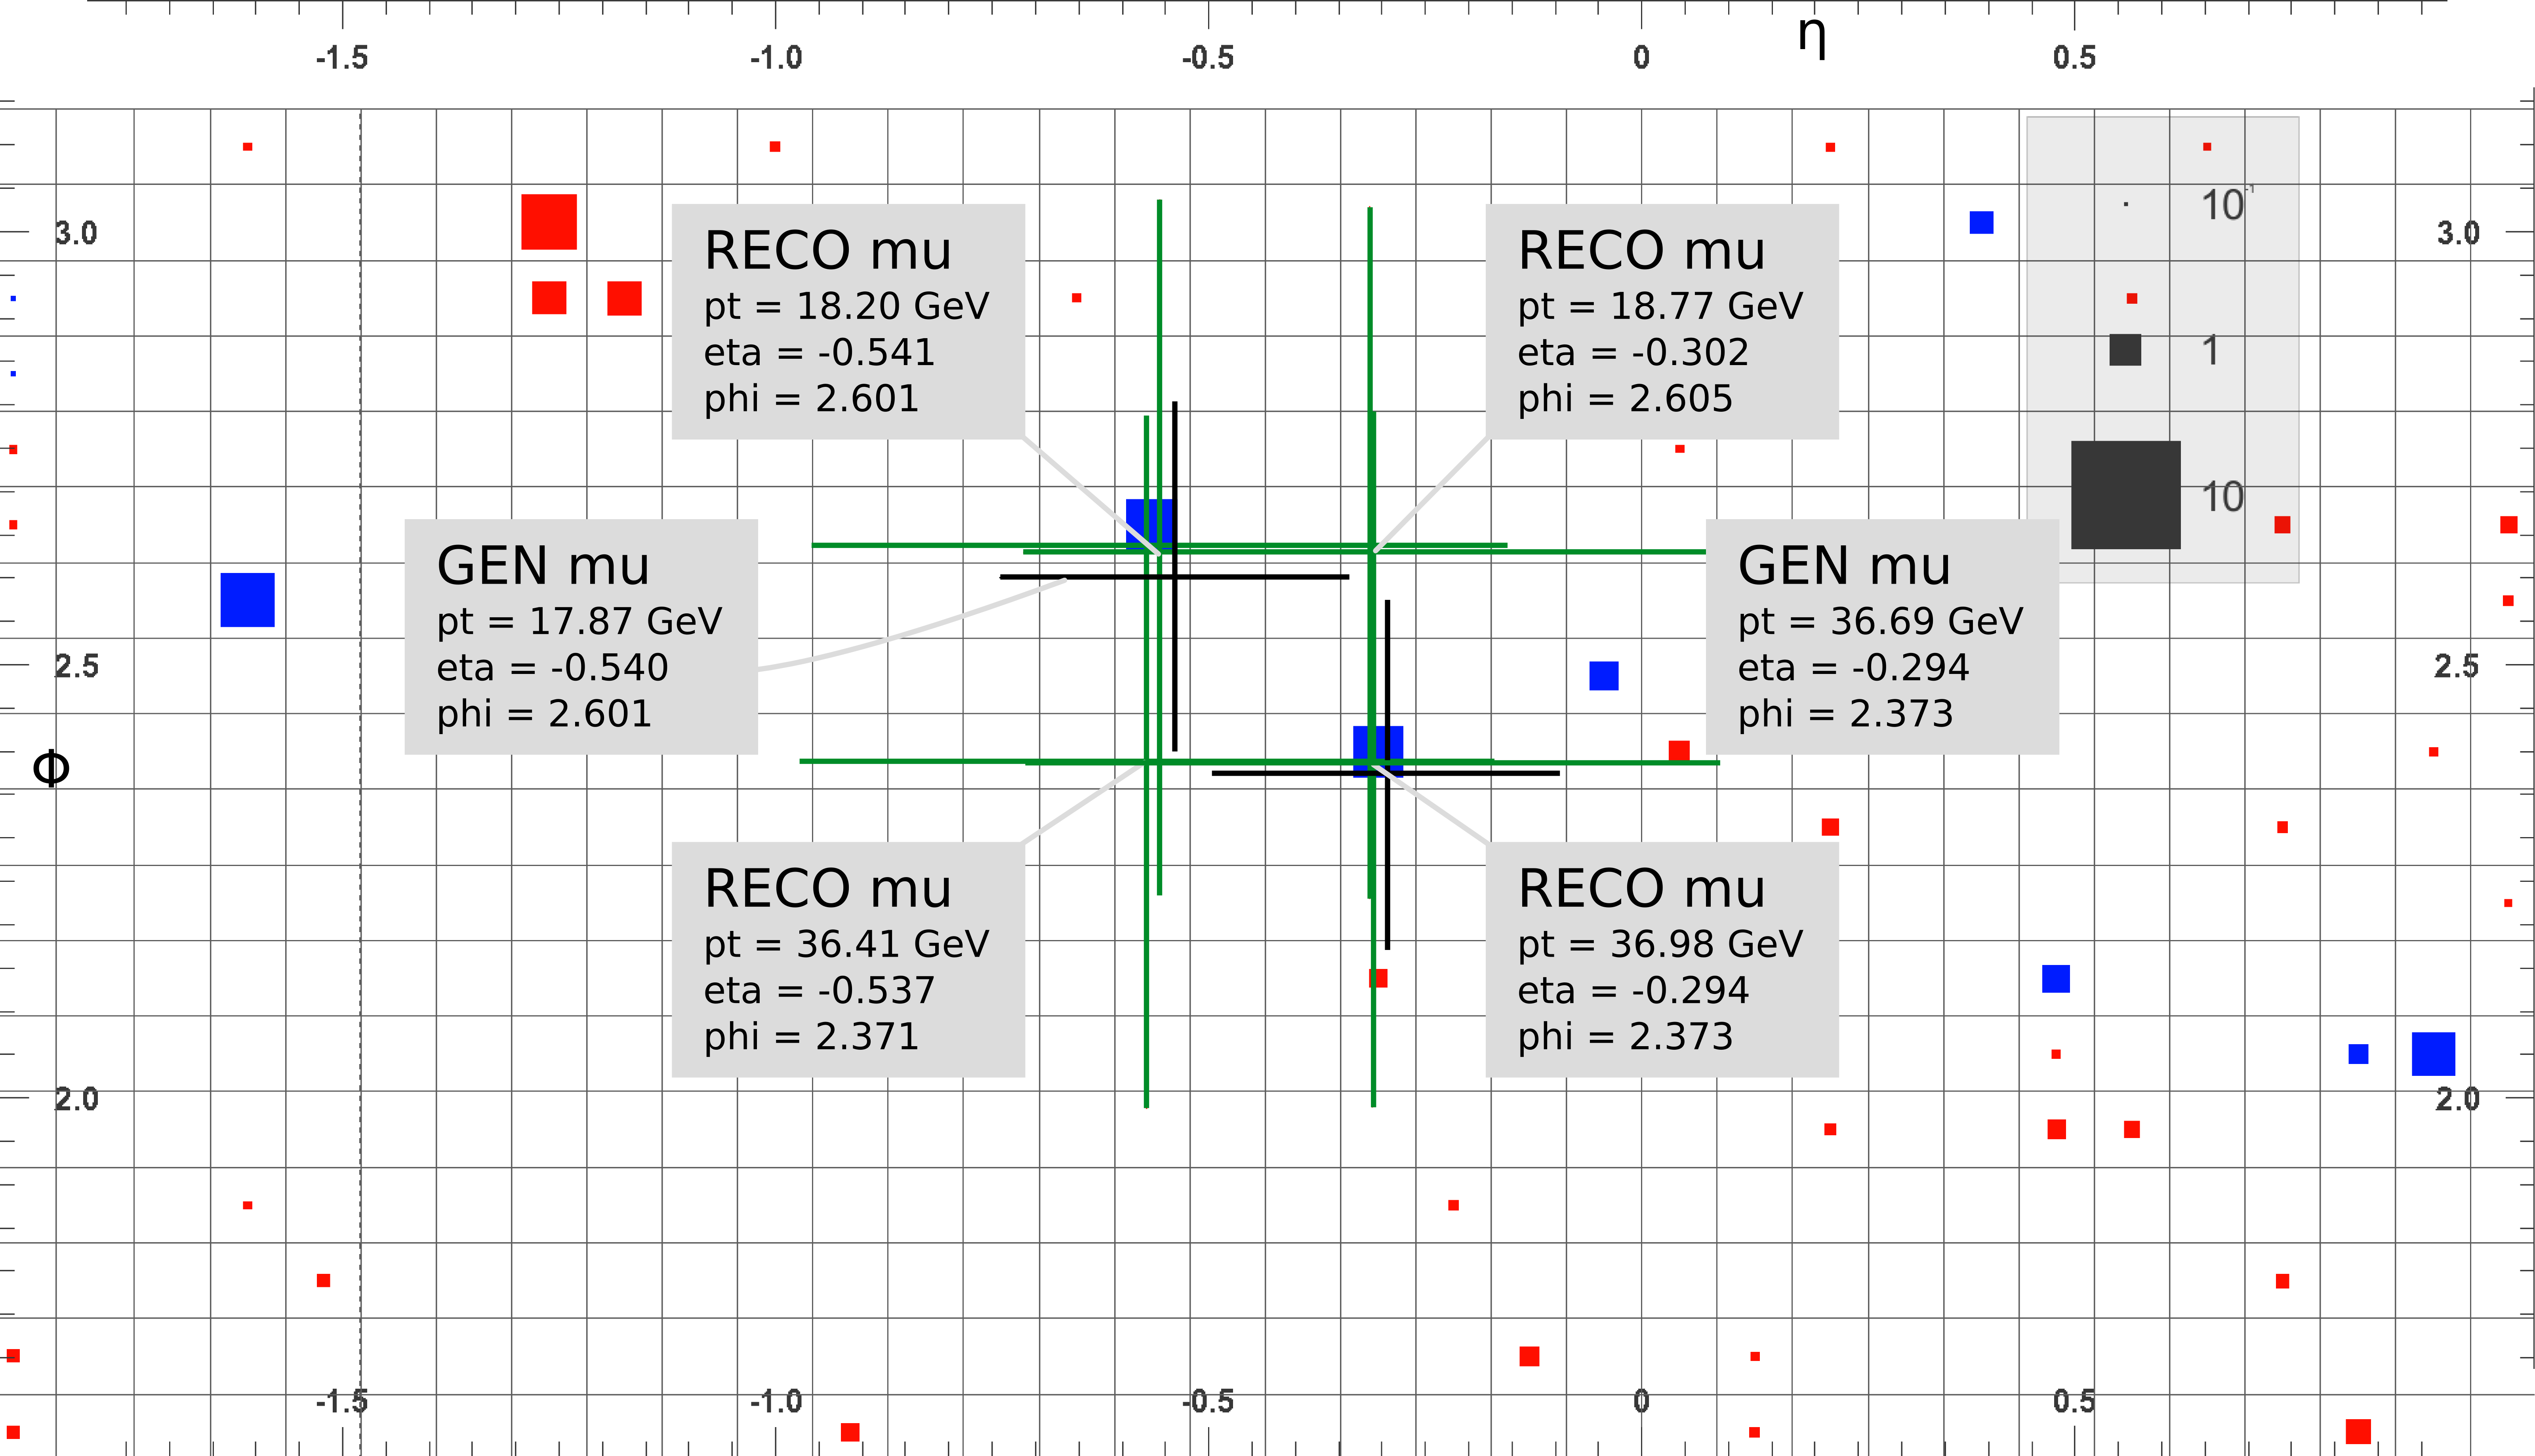
\includegraphics[width=\textwidth]{Figures/pooth/GhostEvent01.png}
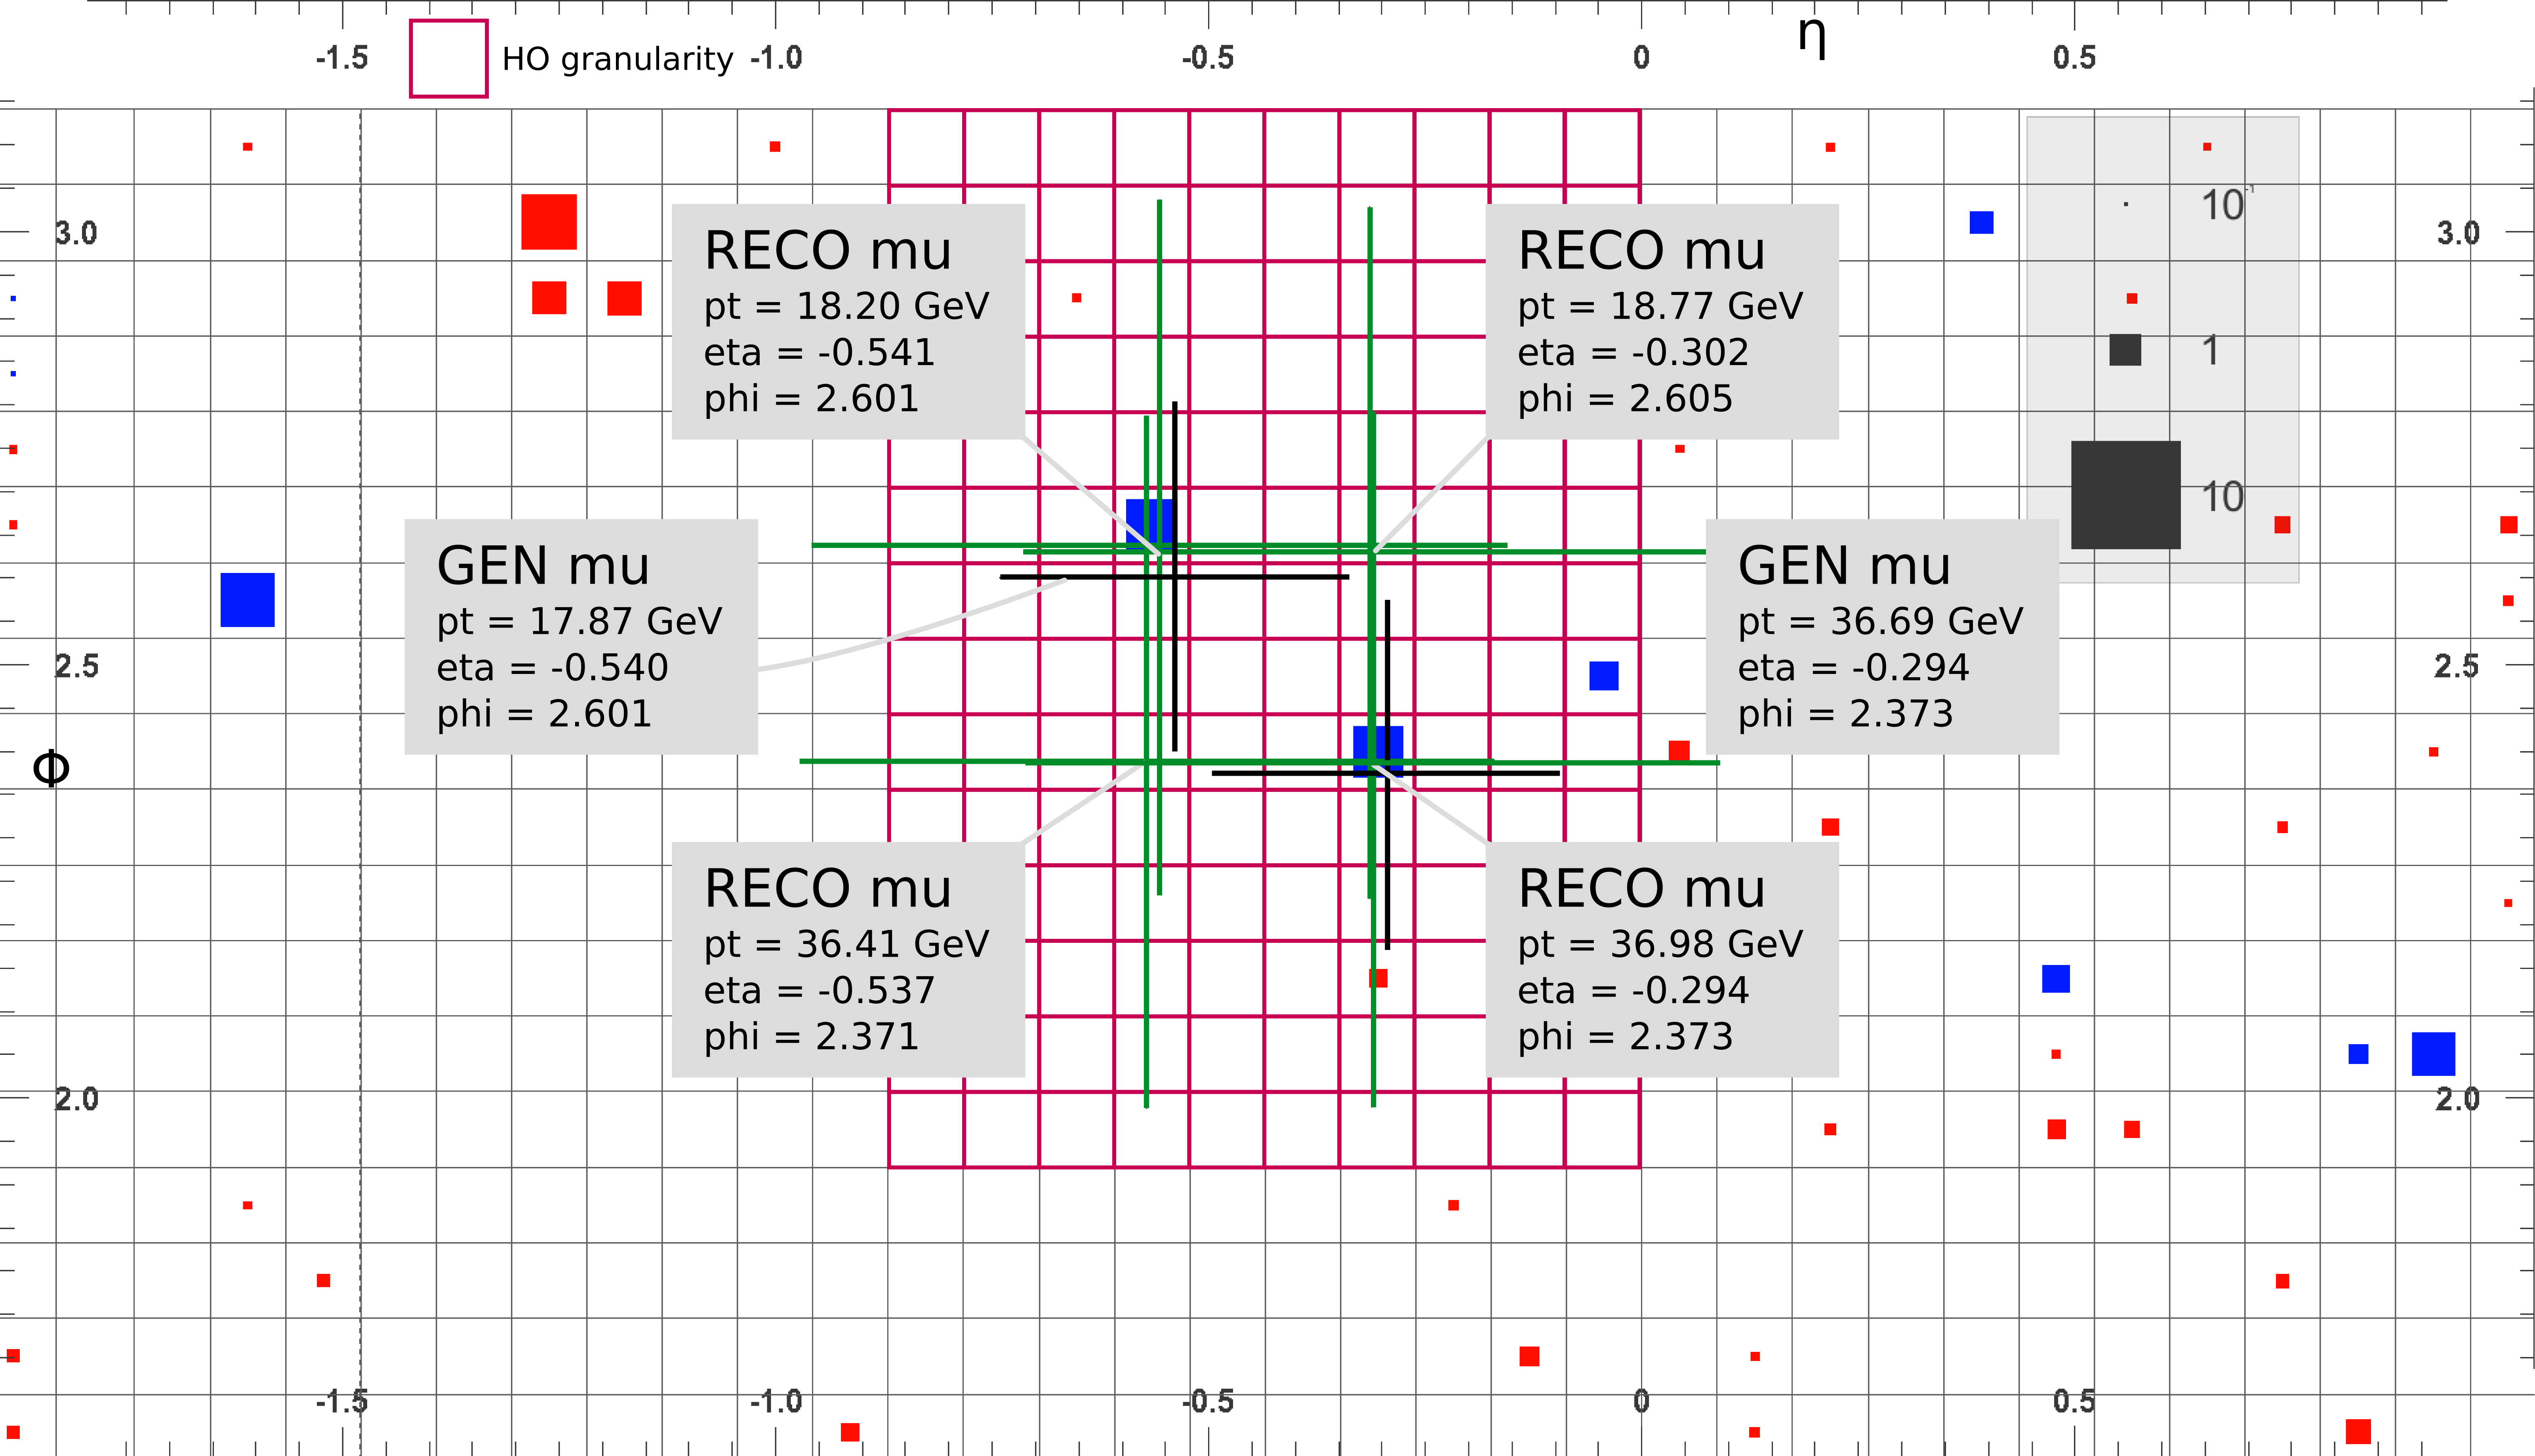
\includegraphics[width=\textwidth]{Figures/pooth/GhostEvent02.png}
\caption{Top: Four reconstructed muons (RECO mu, green crosses) with only two generated muons in the detector (GEN mu, black crosses). 
Bottom: The same event and in addition the HO system overlaid (individual HO tiles shown as pink boxes).} 
\label{fig:ghosts}
\end{figure}
\section{The Hadron Outer Calorimeter}\label{HOintro}
The Outer Hadronic Calorimeter (HO) is a detector system designed for measuring energies of jets that leaked through the solenoid. It consists of scintillator tiles equipped with wavelength shifting fibers. The fibers are put in grooves in a sigma-like shape, as is shown in Fig. \ref{kuenskenScintWithFiber}.
\begin{figure}[h]
\centering
\begin{minipage}[t]{0.475\textwidth}
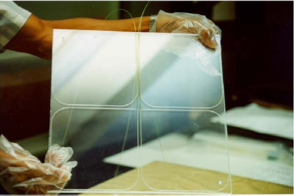
\includegraphics[width=\textwidth]{Figures/kuensken/hoTile.png}
\caption{Scintillator with the wavelength shifting fibers in sigma shape. Image from \cite{hoDesign}.}
\label{kuenskenScintWithFiber}
\end{minipage}
\hspace{1cm}
\begin{minipage}[t]{0.435\textwidth}

\end{minipage}
\end{figure}
From the wavelength shifting fibers the light is coupled into clear fibers to guide the light towards the photo-sensors. The tile's geometry is designed to match the towers of the HCAL in the barrel region which gives a tile size of 0.087$\times$0.087 in eta and phi. The scintillators are placed behind the solenoid in front of the first layer of the iron return yoke. While the rings $\pm$1 and $\pm$2 have only one layer of scintillator, ring 0 has a second layer of scintillator behind the iron yoke. This leads to specialties when bringing the light guiding fibers onto the photo-detectors, as is described in \ref{kuenskenHardwareDesign}.\\
With the upgrade of the photon sensors to SiPMs it is now subject to studies in how far HO has capabilities of detecting muons as Minimum Ionizing Particles (MIP) and providing a discrimination between MIP signals and leaking jets. The muon identification capability may be a key feature when thinking of providing an additional muon tag to the muon trigger system with the help of HO. A more thorough description of HO can be found in \cite{hcalTDR} and \cite{hoDesign}, information on the SiPM upgrade is available in \cite{beniCalor}.

\section{Studies with the Hadron Outer Calorimeter}
In the barrel region of the CMS experiment the hadronic calorimeter has a outer component placed just behind the solenoid and before the first muon stations (BILD). 
This subdetector is called the hadron outer (HO) calorimeter and is a tail catcher for jets leaking out of the inner hadronic calorimeter.
In this section first of all the HO system and its readout structure are introduced.
Then some studies on detection efficiency of muons using 2012 data are shown. The analysis of the detection efficiency for cosmic muons from GRIN data is conclusively dealt with.
	\subsection{The Hadron Outer (HO) Calorimeter}
		to do with Andreas
  		\subsubsection{Benefits and constraints}
			to do with Andreas
  		\subsubsection{Design of the system}
			to do with Andreas
	\subsection{Readout logic and DIGI structure}
		to do with Andreas
  		\subsubsection{Readout setup}
			to do with Andreas
	\subsection{Studies on detection efficiency of prompt muons using 2012 data}
		Due to the similarity of the setup of HO and MTT by studying the HO signals we expect to find answers to some open questions concerning the MTT concept like the muon detection capability of a
		scintillator system  read out by SiPMs e.g. Therefore the detection efficiency for tight ID muons from 2012 data in HO has been studied.
		For this purpose the muons have to fulfill some selection createria and they have to be accepted by the HO system since HO has inefficient areas due to the supporting structures of CMS like the
		chimney (REF).
		\subsubsection{Muon selection and acceptance by HO}
		\label{thesectionhere}
			To be sure to have no fake muons going through the HO tiles some selection createria are set for the reconstructed muons.
			First of all only reco::muons which are also global muons are chosen.
			Then a cut on the pseudorapidity of the muons $|\eta_\mu| < 0.9$ is applied to be ensure that they are in the barrel region and especially in the region of HO.
			The muons also should have a tight ID.
			In (REF) all requirements on muons to be a tight muon are given.
			Essential for the tight ID definition is the consideration of good primary vertices.
			For this purpose a good vertex filter is applied:
			Using the vertex collection \textit{offlinePrimaryVertices} only vertices are chosen whose:
			\begin{enumerate}
				\item minimum number of degrees of freedom is 4,
				\item maximum distance on the $z$ axis to the origin of the coordinate system is 24\,cm,
				\item maximum $d_0$ is 2\,cm.
			\end{enumerate}
			Furthermore all these tight muons have to have an particle flow based combined relative isolation defined as
			\begin{equation}
				\frac{\sum{E_T^{chHad}} + \sum{E_T^{neutHad}} + \sum{E_T^\gamma}}{p_T}
			\end{equation}
			where $E_T^{chHad}$ is the transverse energy of a charged hadron in a cone of $dR = 0.4$ around the muon, $E_T^{neutHad}$ same for a neutral hadron and $E_T^\gamma$ for a photon.
			Since the HO system doesn't cover the whole $\eta$-$\phi$ plane - for example there are no tiles between the wheels - and also since the HO system has some areas with elecronic inefficiencies the
			cut on $|\eta_mu|$ mentioned before is not sufficient and a more sophisticated geometrical acceptance have to be requiered. 
			This is done using the \textit{MuonHOAcceptance} class implemented in the software framework of CMS.
			\textit{MuonHOAcceptance} knows the entire HO geometry and allows boolean decisions on whether a muon is in the geometrical acceptance of the HO or not and also whether a muon is in the acceptance region of
			tiles which are working properly.
			It is also possible to accept or reject muons in regions with SiPM instrumented tiles (figure ho_acceptance).
			\begin{figure}[htbp]
				\centering
				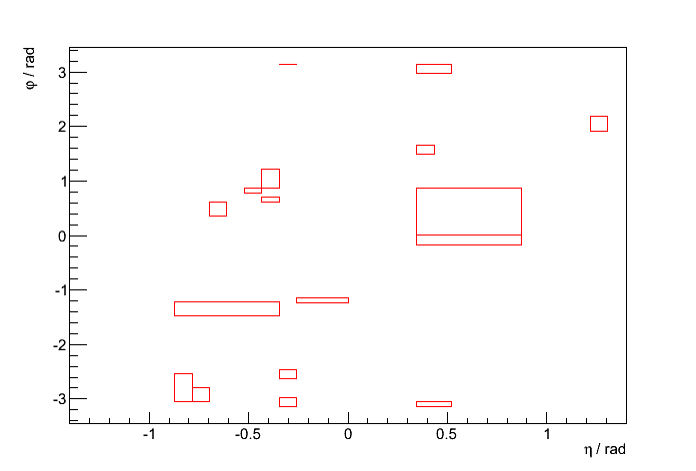
\includegraphics[width=0.45\textwidth]{Figures/erdogan/deadregions.png}
				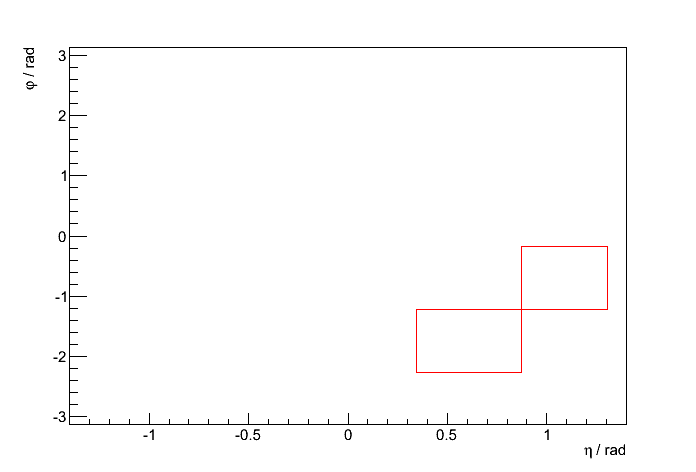
\includegraphics[width=0.45\textwidth]{Figures/erdogan/sipmregions.png}
				\caption{Left: In the $\eta$-$\phi$ plane, the red rectangles are showing the regions where HO is insensitive due to the supporting material or electrical issues. Right: In red rectangles the
				acceptance regions for tiles with SiPM readout.}
				\label{fig:ho_acceptance}
			\end{figure}
			In figure (simhits_in_acceptance) the $\eta$-$\phi$ distribution of simulated hits of muons with $p_T = 100$\,GeV (muon gun) in HO is shown.
			According to it a large fraction of the accepted muons deposit energies predicted by Bethe-Bloch.
			But there are muons going through HO tiles but depositing very low energies or no energy at all.
			These muons are located particularly at the edges of the HO panels.
			Having only scratched the HO tiles barely, the transition is only enough for either very low depositions or nothing.
			Therefore it is helpful to reject muons flying in these regions by defining safety distances from the edges of the panels as it is shown on the right hand side in figure (simhits_in_acceptance).
			\begin{figure}[htbp]
				\centering
				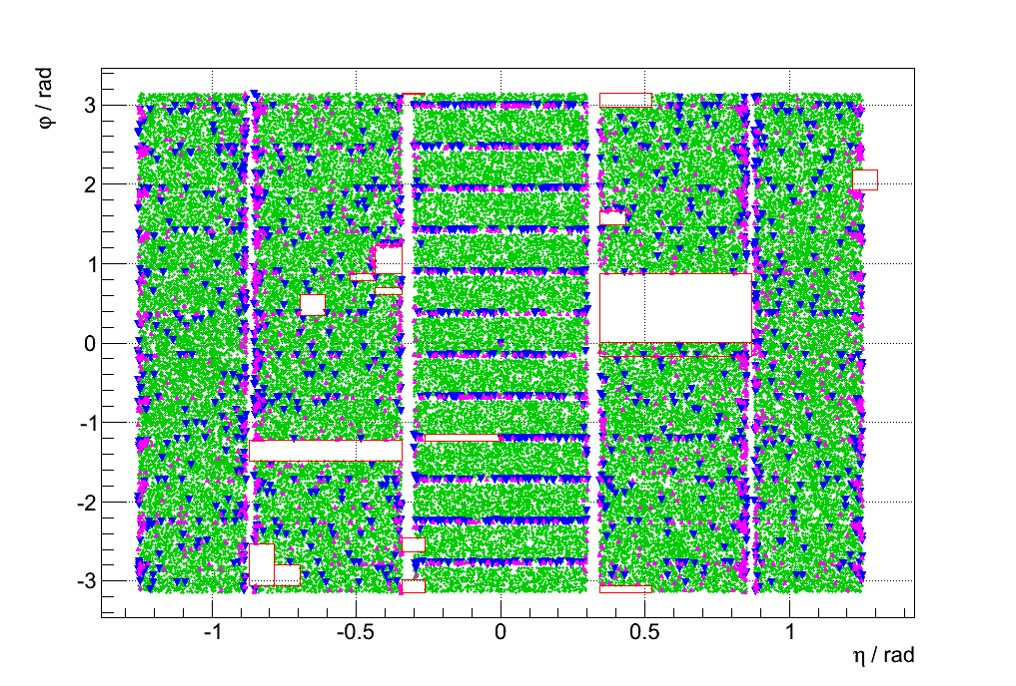
\includegraphics[width=0.45\textwidth]{Figures/erdogan/simhits_wo_deta_dphi.png}
				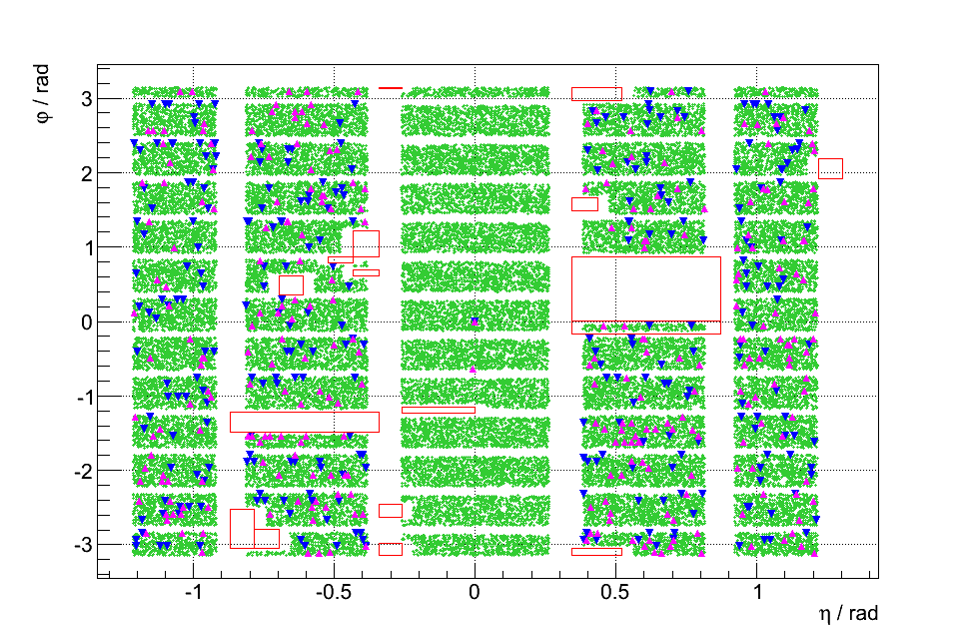
\includegraphics[width=0.45\textwidth]{Figures/erdogan/simhits_with_deta_dphi.png}
				\caption{Left: $\eta$-$\phi$ distribution of simulated hits of muons with $p_T = 100$\,GeV (muon gun). In green, hits from geometrically accepted muons with energy depositions above 1.4\,MeV, in
				blue, same for muons with energy depositions between 0 and 1.4\,GeV and in magenta, for muons with no energy deposition at all. The threshold at 1.4\,MeV is motivated by Bethe-Bloch formula, which
				predicts an energy deposition of > 1.4\,MeV for muons going through 1\,cm material (REF). Right: The same distribution with the safety distances from the edges of the HO panels.}
				\label{fig:simhits_in_acceptance}
			\end{figure}
			By having these safety distances there is only a very small fraction of muons depositing low energies with uniform $\eta$-$\phi$ distributions in the panels due to the insensitive areas between
			the tiles.
		\subsubsection{Matching of the muons to the corresponding HO tiles}
			Being selected as in \ref{thesectionhere} described the muons now have to be matched to the correct HO tiles.
			This is done by using the standard tracking tool \textit{TrackDetMatchInfo}.
			Doing a helix approximation this tool collects the information along a track.
			Among this information also HO related parts like the detector IDs of the tiles crossed by the muon, the reconstructed hits in these tiles or the global position of the track at HO etc. can be
			found.
			If one of the IDs of the tiles crossed by a muon is the same as one of the IDs of a reconstructed hit in the HO system, then this muon is matched to that tile.
			Since no additional requirements like to have a certain energy e.g. on the reconstructed hits are done, this procedure is a very loose one.
		\subsubsection{Detection efficiency for prompt muons}
			todo
	\subsection{Studies on detection efficiency of cosmic muons using the GRIN data} 
		todo
		\subsubsection{Detector setup for the Global Run In November (GRIN)}
			todo
		\subsubsection{Purity studies}
			todo
		\subsubsection{Efficiency studies}
			todo
		\subsubsection{Working point for triggering muons}
			todo

\section{MTT Simulation Studies}
\label{sec:MTTsimulation}
	For future physics studies with MTT impact, this system has to be implemented in the standard CMS geometry description within CMSSW.
	In this section this implementation is described. 
	\subsection{MTT Geometry in CMSSW}
		\subsubsection{The geometry model of CMS}
			The geometry model of CMS is based on Geant4 \cite{Geant4}.
			It is constructed hierarchically and realized by the XML based detector description language \cite{CMSDDL}.
			To make the geometry available on runtime the ESProducer \verb+XMLIdealGeometryESSource+ is used converting the XML description of the geommetry in a C++ model.
			The tree structure of the geometry is then available in the event as an instance of the \verb+DDCompactView+.
			In general there are two main classes of geometries in CMS.
			For the tracking systems like the muon subdetectors and tracker etc. tracking geometries are available.
			For the calorimeter systems one can use the calorimetry geometry classes.
			Details on this procedure can be found in \cite{CMSDDL}.
			For alternative geometry models like the extended CMS geometry containing the MTT system it is nessessary to modify \verb+XMLIdealGeometryESSource+ to load corresponding XML
			files.
			In the next section the XML based geometry description of the MTT system is explained.
		\subsubsection{Description of the MTT geometry for different scenarios}
			\subsubsection*{General:}
			All parts of the MTT geometry are arranged in a hierarchy, which is very similar to the muon system hierarchy, especially of the DT system.
			Concerning this the MTT geometry is to be assigned to the class of tracking geometries.
			Furthermore the local coordinate system of MTT is chosen in a way, that the z axis concurs with the global z axis of CMS.
			The local y axis is therefore pointing outwards radially.
			\subsubsection*{Inner Hierarchy:}
			The basic unit of the MTT geometry is the \verb+MTTTile+.
			This unit is consisting of a scintillator of 10\,mm thickness wrapped by a polyethylene layer of 1\,mm thickness.
			In Figure \ref{fig:tile_wowrapping} several scintillators are seen in light green.
			The sensitive material of the scintillator is a generic hydrogencarbon compound with the mass composition of $m_H:m_C \approx 91.5\,\%:8.5\,\%$.
			\begin{figure}[htbp]
				\centering
				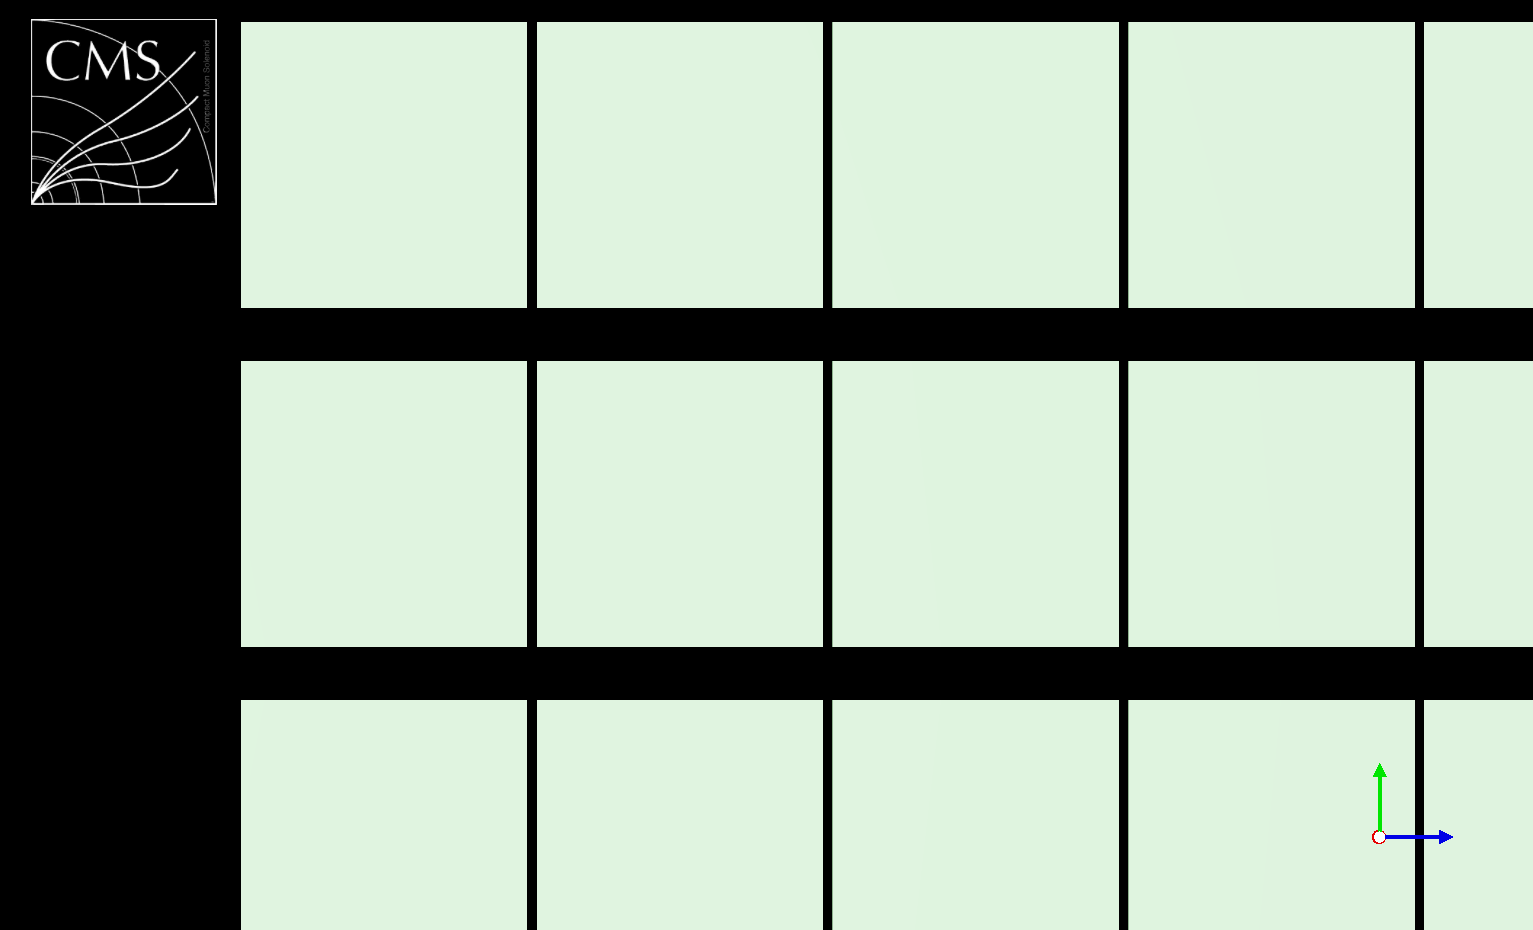
\includegraphics[width=0.70\textwidth]{Figures/erdogan/tile_wowrapping.png}
				\caption{MTT geometry: tiles without wrappings.}
				\label{fig:tile_wowrapping}
			\end{figure}
			The gaps in between are on the one side due to the absence of the wrapping and on the other side due to the placing in the superior detector unit called \verb+MTTStrip+.
			Several \verb+MTTTiles+ namely can be arranged along the z axis in these strips (Fig. \ref{fig:strip}).
			\begin{figure}[htbp]
				\centering
				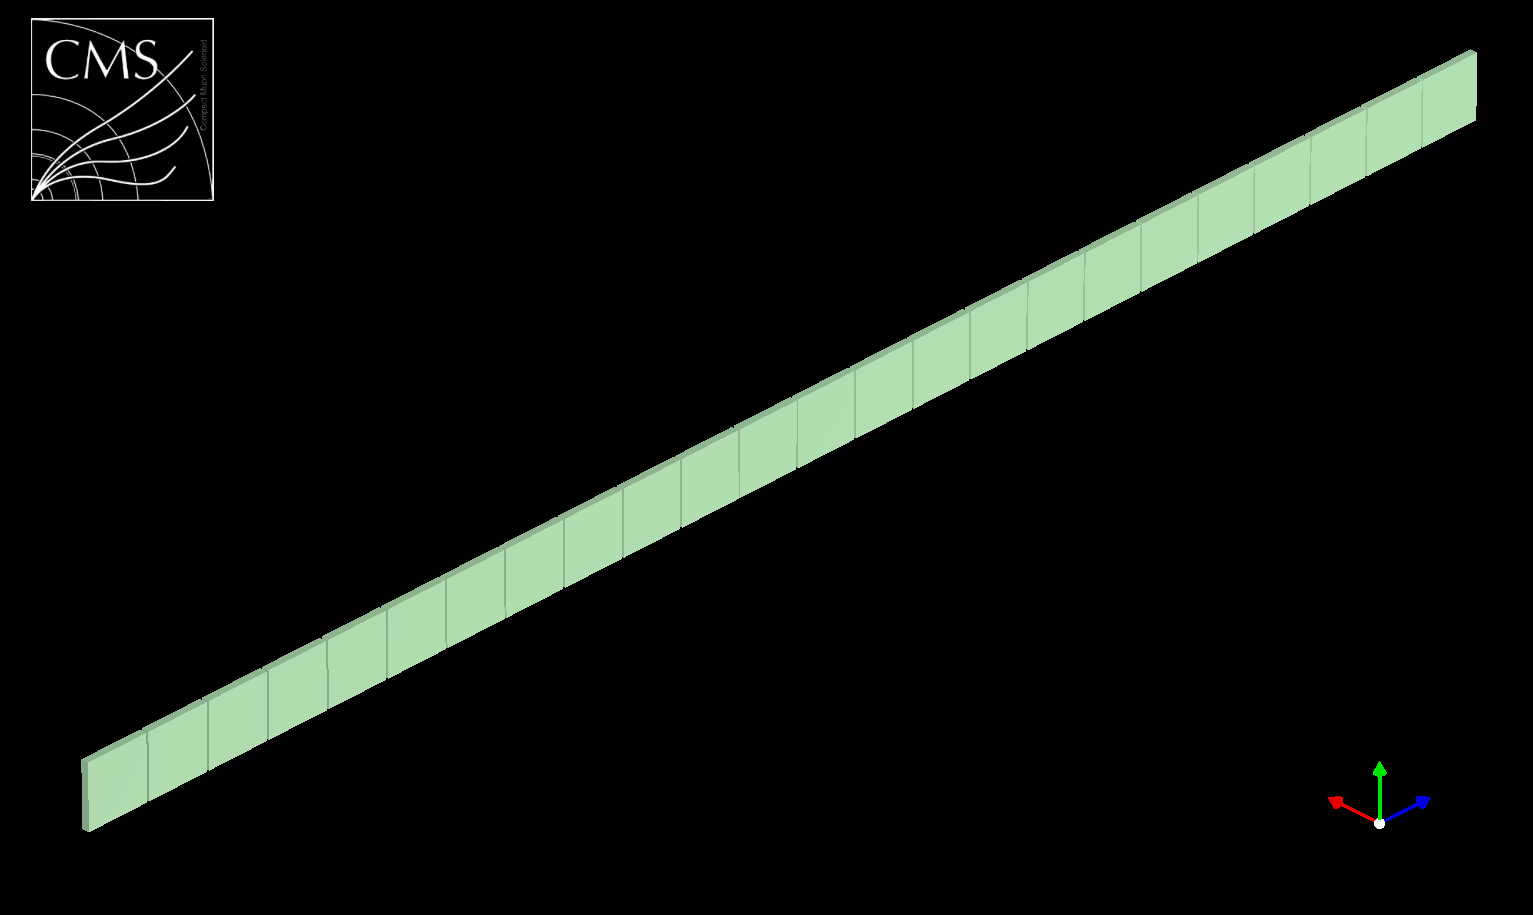
\includegraphics[width=0.70\textwidth]{Figures/erdogan/strip.png}
				\caption{MTT geometry: array of several tiles, called strip.}
				\label{fig:strip}
			\end{figure}
			The dimensions of the tiles are dynamic and determined automatically to be fit in a \verb+MTTStrip+ in a way that a strip contains the number of tiles given by the user having the insensitive areas
			between the tiles to be minimal.
			The dimension of a strip is fixed in z direction at 2536\,mm since this is the width of the wheels.
			This constraint is the reason of the insensitive areas between the tiles.
			However in a more sophisticated geometry description these areas can be minimalized since the implemented geometry is a first try to check the feasibility. 
			The strip itself is made of polystrene.
			An array of strips in local x direction is called a layer (Fig. \ref{fig:layer}).
			\begin{figure}[htbp]
				\centering
				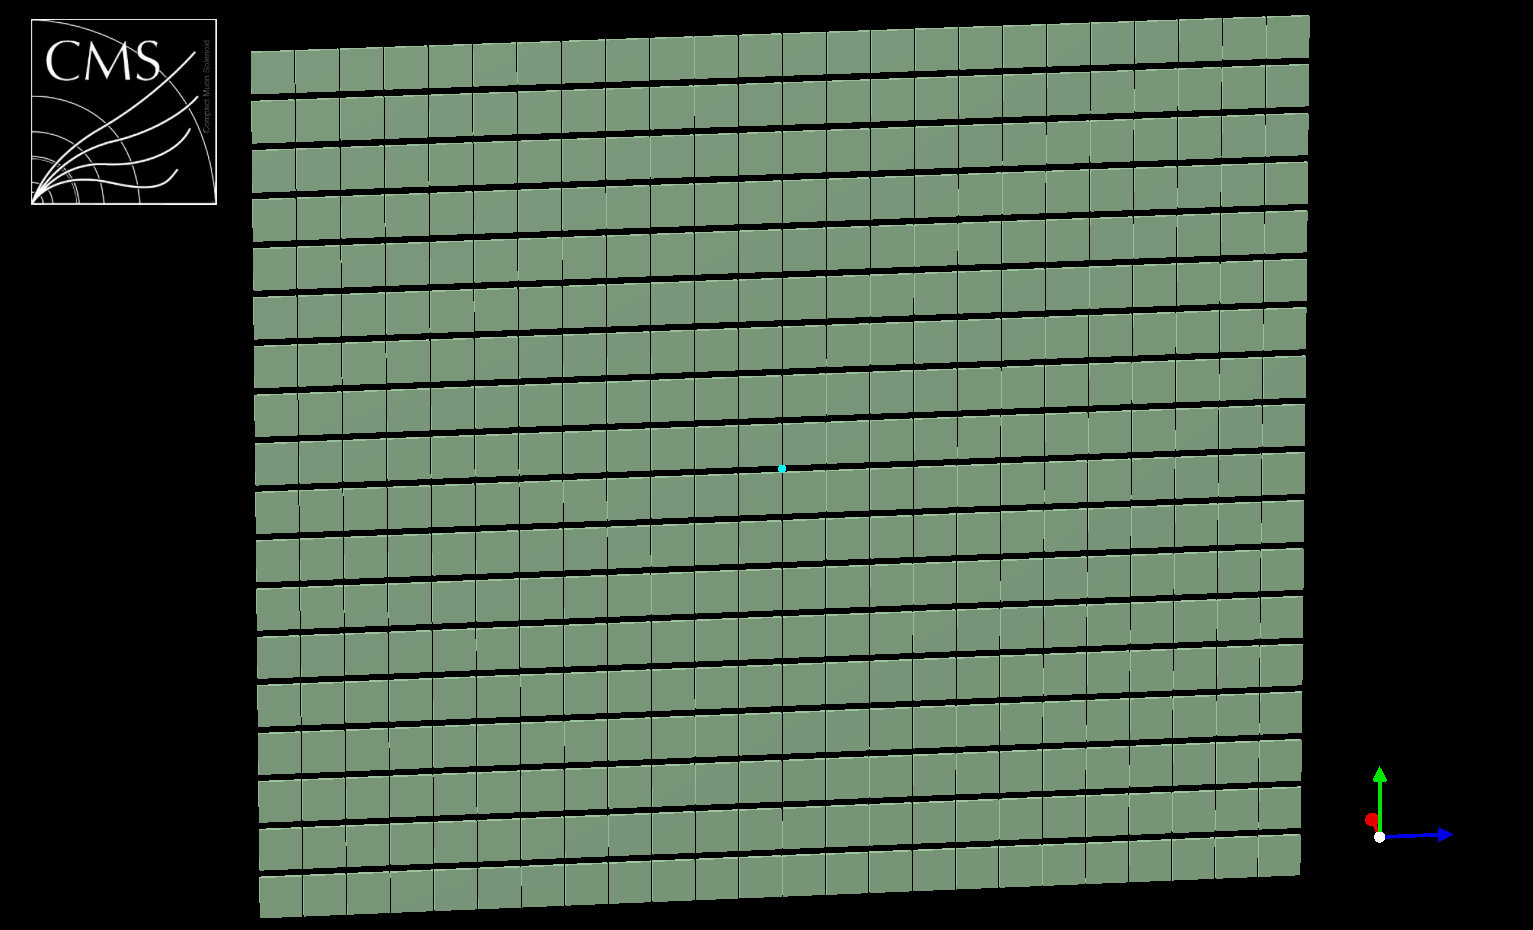
\includegraphics[width=0.70\textwidth]{Figures/erdogan/layer.png}
				\caption{MTT geometry: array of several strips, called layer.}
				\label{fig:layer}
			\end{figure}
			Several layers in y direction can be arranged in a panel, which is the top unit in the hierarchy.
			There are already different scenarios written for MTT geometry having one or more layers in a panel (Fig. \ref{fig:panel}).
			\begin{figure}[htbp]
				\centering
				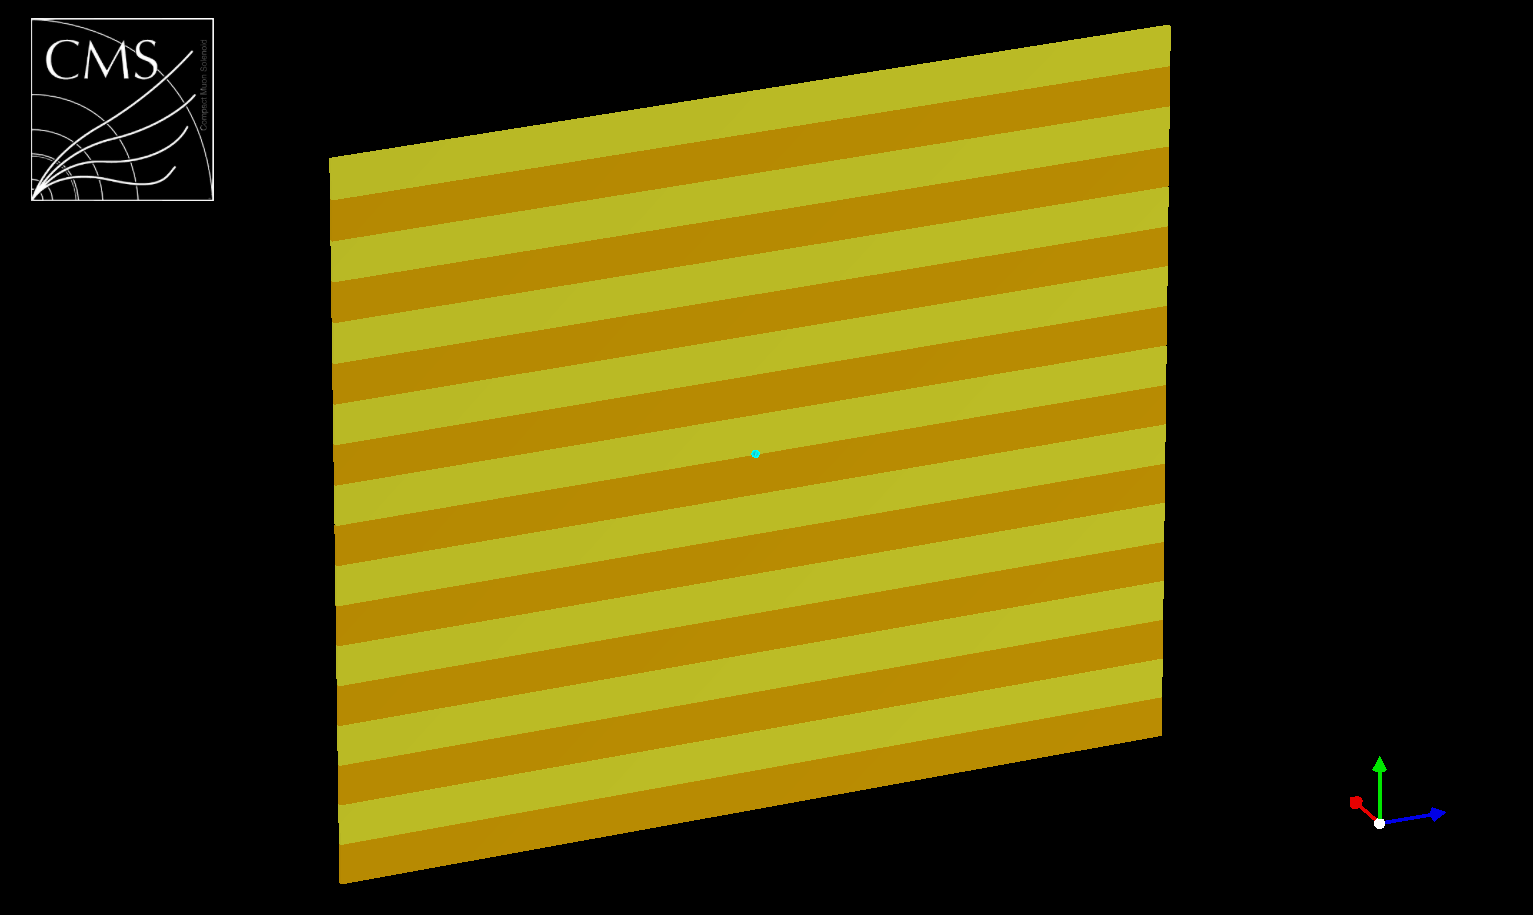
\includegraphics[width=0.45\textwidth]{Figures/erdogan/panel1.png}
				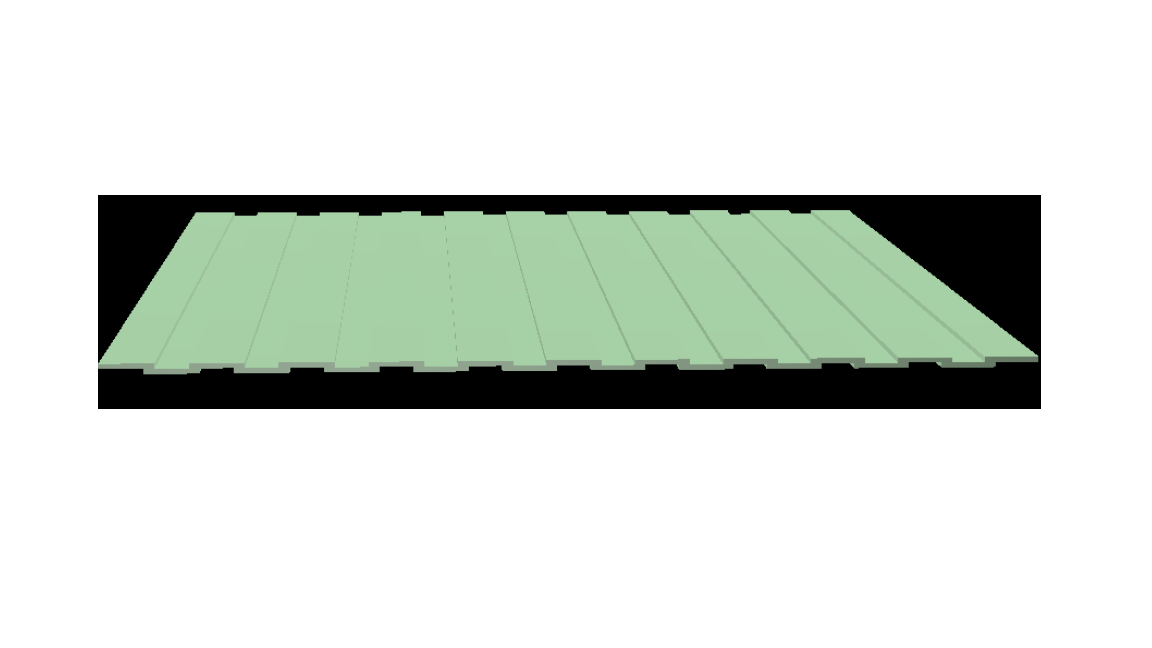
\includegraphics[width=0.45\textwidth]{Figures/erdogan/panel2.png}
				\caption{left: one \verb+MTTPanel+ with one layer, right a possible scenario for one panel with two layers.}
				\label{fig:panel}
			\end{figure}
			\subsubsection*{Numbering:}
			In the detector description of CMS, each detector unit is unique by a 32 bit integer named the DetId.
			The composition of this integer is depicted in Fig. \ref{fig:numbering}.
			\begin{figure}[htbp]
				\centering
				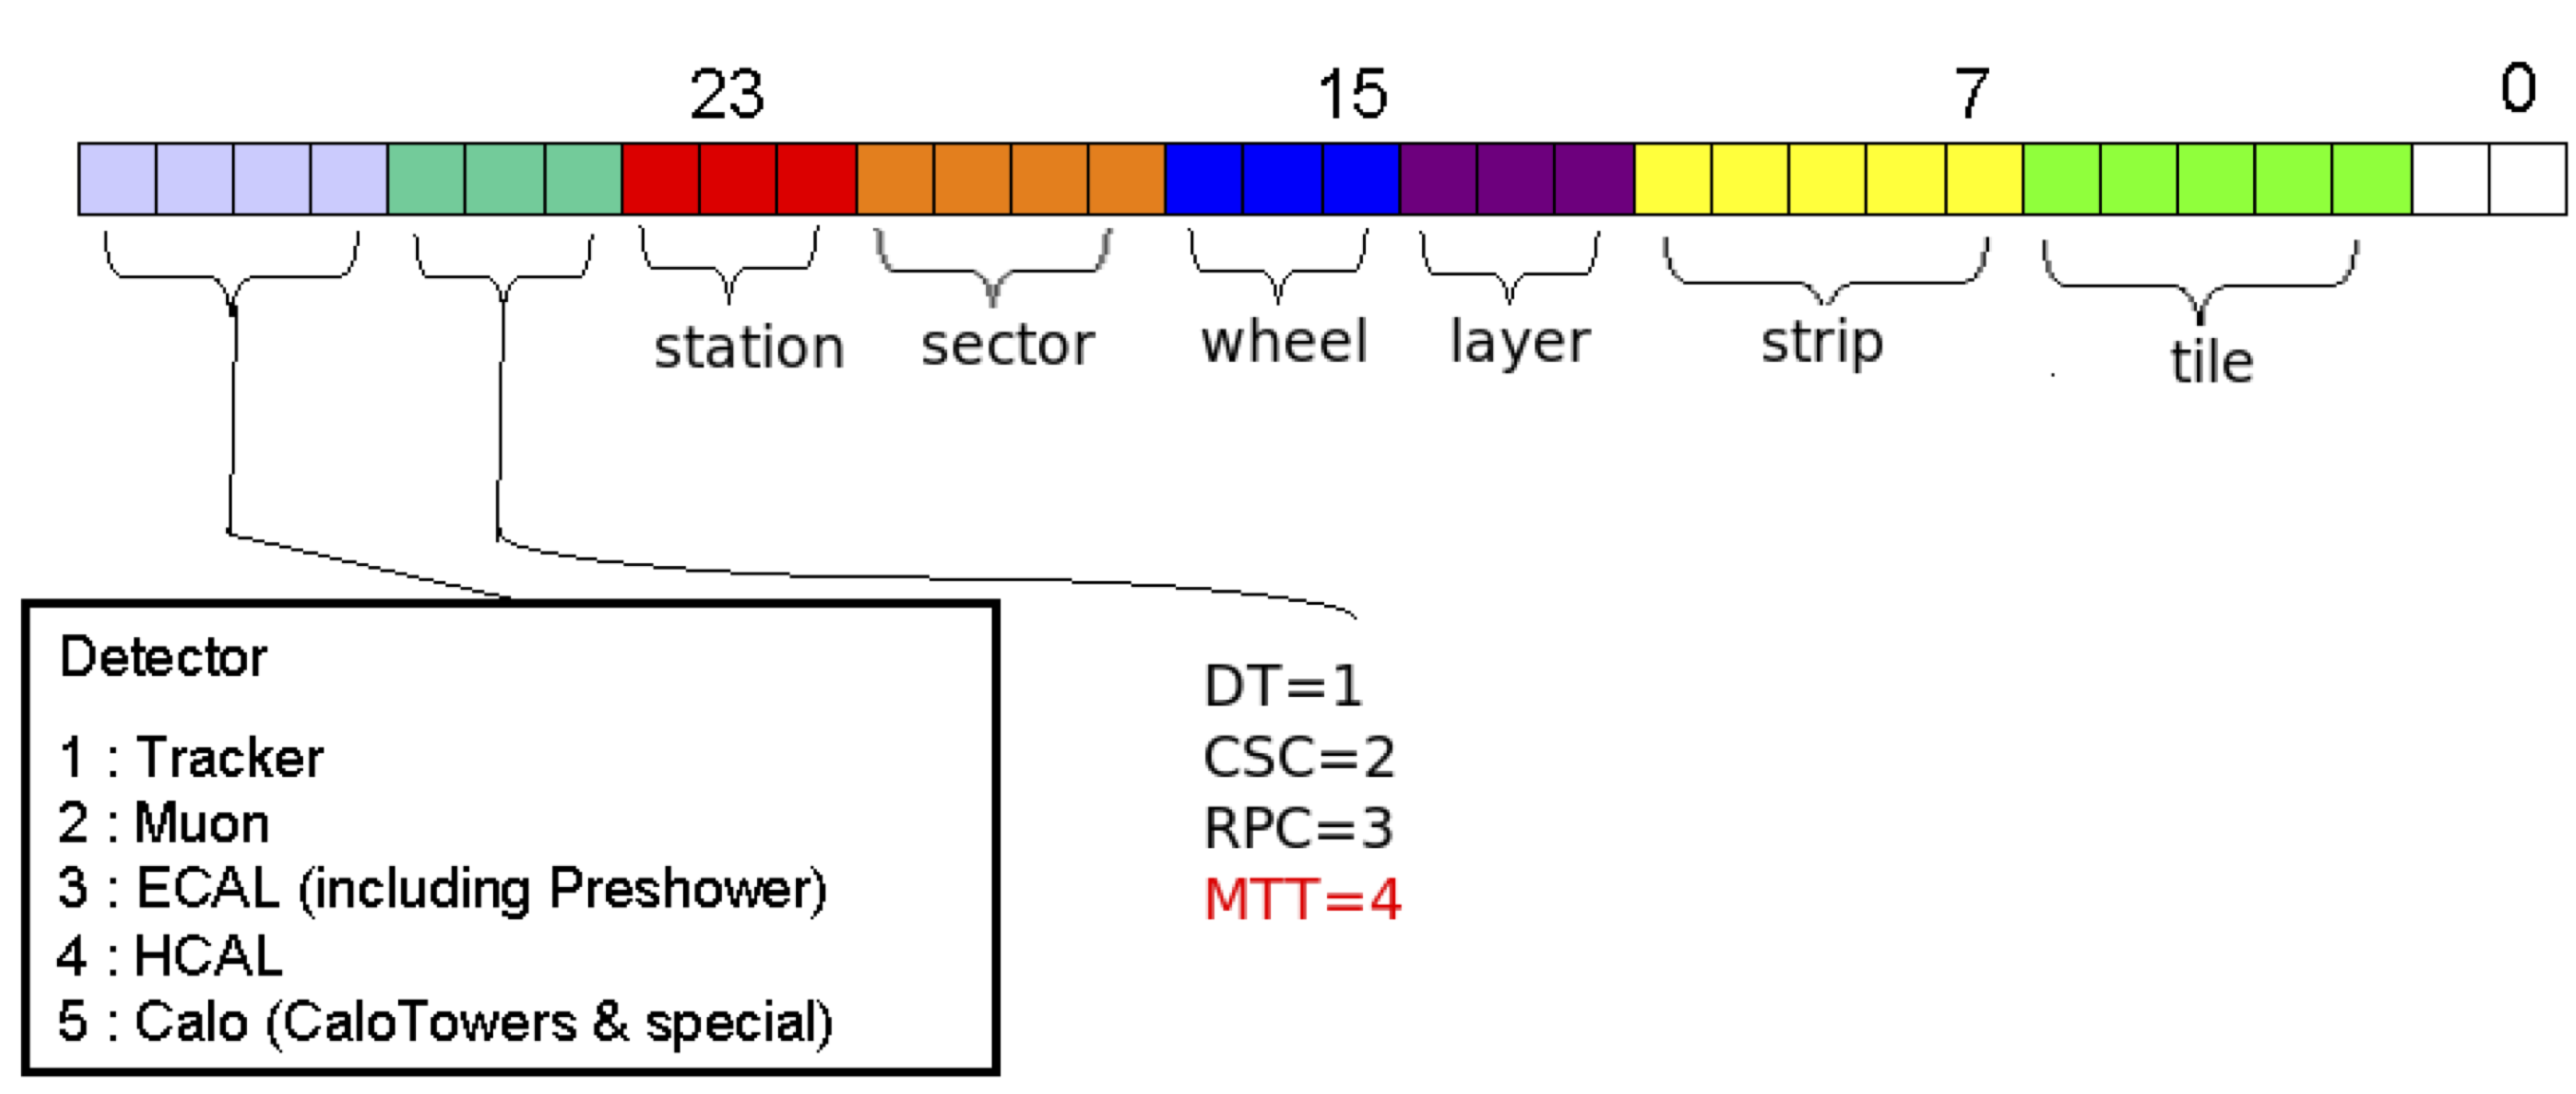
\includegraphics[width=0.70\textwidth]{Figures/erdogan/numbering.png}
				\caption{Unique numbering scheme of CMS detectors units.}
				\label{fig:numbering}
			\end{figure}
			The first four bits are reserved for the subdetector to which the considered detector unit belongs to.
			The following three bits are marking the subsystem within the subdetector, like DT, CSC, RPC or in our case MTT within the muon system.
			The remaining bits are used to desribe the location of the detector unit in a certain wheel, station etc.
			For MTT we used the three bits after the bits for the subsystem, for the station, four bits for the sector, three bits for the wheel, three bits for the layer, five bits for the strip and five bits
			for the tile.
			With this a MTT system consisting of seven layers each with 31 strips per $\varphi$-sector can be numbered consecutively in a unique way.
			This would allow tiles with only a few cm$^2$ surface area and since the planned MTT tiles are around 10$\times$10\,cm$^2$ this numbering is more than sufficient.
		\subsubsection{Setup and verification for the SimHit generation}
			After having the geometry of MTT within the CMSSW the next step is to create tools to simulate hits when particles go through a MTT tile.
			This task is handled by the \verb+MTTSensitiveDetector+ tool, which is based on the Geant4 counterpart SensitiveDetector.
			\verb+MTTSensitiveDetector+ collects the information like energy loss, time of flight or position step by step and stores it in a hit.
			Afterwards this tool has to be introduced to the general hit producer within CMSSW named the \verb+OscarProducer+.
			The \verb+OscarProducer+ is responsible for producing hits in several subdetectors at the beginning of an event.
			This is called the SIM step.
			(Furthermore the OscarProducer gives the subdetector algorithms constraints like energy thresholds etc.)
			To verify the correct behaviour of the MTT simhit generator, one can look at the position of the hits in the MTT tiles.
			For this purpose a muon gun placed in the point of origin of CMS was fired uniformly in all directions and the the x and y coordinates of the simulated hits in MTT were plotted (Fig.
			\ref{fig:hitpos_mtt}).
			\begin{figure}[htbp]
				\centering
				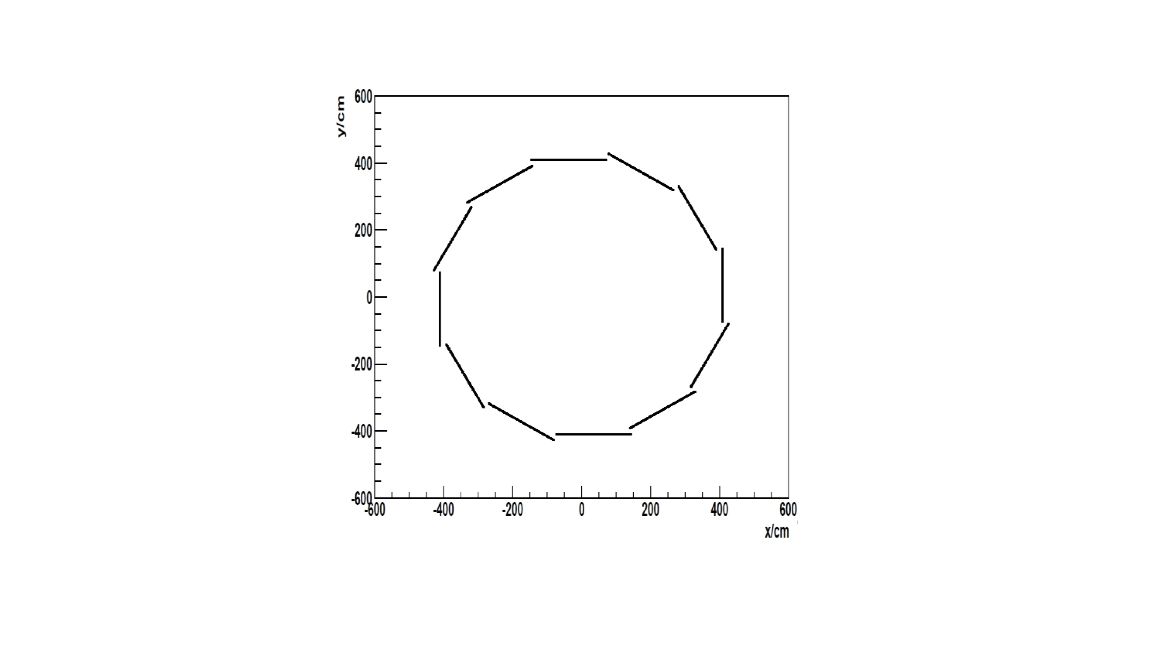
\includegraphics[width=0.70\textwidth]{Figures/erdogan/hitpos_mtt.png}
				\caption{Position of the hits simulated in the MTT in the x-y plane (from \cite{paul_thesis})}
				\label{fig:hitpos_mtt}
			\end{figure}
			The width of the 12 MTT panels in 12 $\varphi$ sectors can be seen at a distance of approximately four meters in x and y direction.
		\subsubsection{DIGI generation}
			The simulation of the hits with Geant4 based tools does not consider the detector response on the electronics site.
			This information has to be added to the simulation.
			This is called the DIGI step.
			Since the MTT tiles are under development and the front end electronics are not finalized yet, only a dummy digitizer could be written for MTT.
			In this dummy for each SimHit a DIGI is applied without any constraint on its parameters like energy or inefficiencies on the electronics site e.g. photon detection efficiency of the SiPMs etc.
			Nevertheless this digitizer is very important for the future analyzes since the MixingModule of CMSSW requires a digitizer to mix pile up information to the signal.
			Only with this it is possible to analyze the HL-LHC conditions with high pile up and with the extended CMS geometry by MTT.
%\subsection{First SimHit studies and their results}
	%All in this section shown first results are described in detail in (PAULREF).
	%As explained in the introduction chapter the main tasks for MTT would be the assignment of standalone muon tracks from the muon system to the tracks from track trigger (REF).
	%Therefore we have investigated the detection efficiency of L1Tracks in the MTT system.
	%However since the MTT system has only one layer with only 1 cm thickness, we don't expect very high efficiencies like the CMS muon system with its 4 stations and 4\,m lever arm can provide.
	%It is rather a feasibility analysis to see first hints of geometrical inefficiencies of the MTT.
	%In figure (REF) the matching efficiency as a function of transverse momentum $p_t$ of muons is depicted.
	%For this analysis a muon gun were used as described in the previous section.
\section[HO SiPM upgrade]{HO SiPM upgrade\footnote{Corresponding Author: Andreas K\"unsken}}\label{sec:hoSipmUpgrade}
\subsection{Hardware design}\label{kuenskenHardwareDesign}
In the first long shutdown of the LHC, HO was subject to upgrades. The previously used Hybrid Photo-Diodes (HPD) were replaced by SiPMs due to bad performance. The SiPM readout was designed as a drop-in replacement to keep most of the readout chain. The SiPMs were arranged on a newly produced Printed Circuit Board (PCB) to match the position of the pixels of the HPDs. The arrangement of the SiPMs is shown in Fig. \ref{kuenskensipmPcb}.
\begin{figure}[htbp]
\centering
\begin{minipage}[t]{0.475\textwidth}
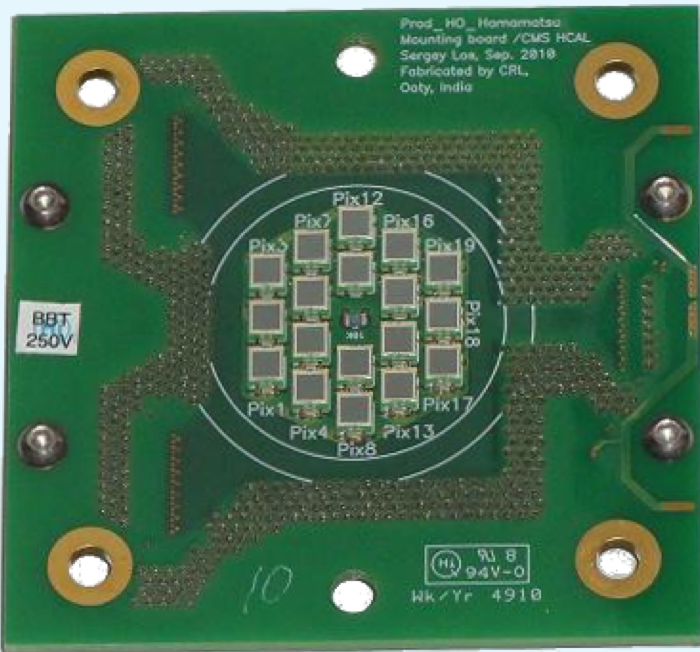
\includegraphics[width=\textwidth]{Figures/kuensken/pcbSipm.png}
\caption{PCB carrying 18 SiPMs. The white cirlce marks the position of the removed HPDs. Image adapted from \cite{beniCalor}.}
\label{kuenskensipmPcb}
\end{minipage}
\hspace{1cm}
\begin{minipage}[t]{0.435\textwidth}
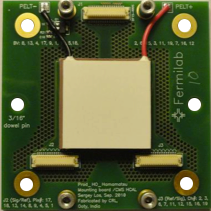
\includegraphics[width=\textwidth]{Figures/kuensken/pcbPeltier.png}
\caption{Backside of an HO PCB with the Peltier element attached. Image adapted from \cite{beniCalor}.}
\label{kuenskenpeltier}
\end{minipage}
\end{figure}
It can be seen that the new PCB has 18 SiPMs in the position where the 18 pixels of the HPDs were located.
The installed SiPM type was produced by Hamamatsu and is identical to a Hamamatsu S10931-050. It has an area of (3x3)\,mm$^2$ and comes with an SMD type housing. The cell pitch is 50\,$\mu$m.
Because HO has two layers of scintillator in ring 0 the number of fibers arriving at a single SiPM is larger in ring 0. As a consequence, the fibers cannot be arranged such that they completely fit inside the area of an SiPM. Therefore, a light mixer is installed between the ends of the fibers and the SiPM surface in ring 0. This light mixer
ensures that the light is distributed uniformly over the SiPM's surface, thus, avoiding the loss of light of only certain fibers.\\
SiPMs are solid state devices and rather sensitive to temperature changes, it is inevitable to provide a controlled temperature environment for a stable operation of the devices. A key feature is the change of the SiPM's breakdown voltage with temperature. The manufacturer specifies this quantity to 56\,$\frac{\text{mV}}{\text{K}}$. For this reason the PCBs carrying the SiPMs are equipped with Peltier elements on their backsides. Fig. \ref{kuenskenpeltier} shows a mounted Peltier element on a PCB.
\subsection{System performance}
\subsubsection{Temperature}
The performance of an SiPM changes strongly with the temperature if not corrected for. For this reason it is important to control the temperature of an SiPM before studying other parameters to make sure that any observed change is not due to a change in the temperature. Figure \ref{kuenskentemperatureStability} shows temperature deviations from a reference temperature plotted versus time.
\begin{figure}[htbp]
\centering
\begin{minipage}[t]{0.475\textwidth}
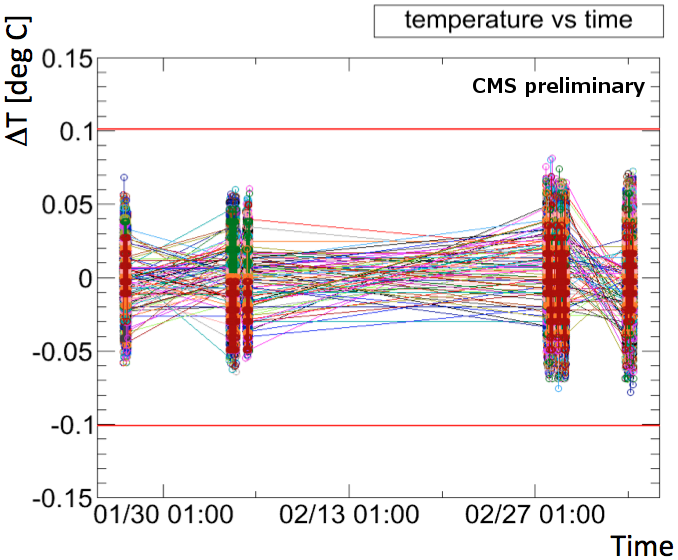
\includegraphics[width=\textwidth]{Figures/kuensken/temperature.png}
\caption{Fluctuation of temperature at the PCBs plotted versus time. The data points represent the temperatures at the PCBs for a given time. Fluctuations stay within 0.1\,$^\circ$C \cite{kuenskenCalor}.}
\label{kuenskentemperatureStability}
\end{minipage}
\hspace{0.5cm}
\begin{minipage}[t]{0.455\textwidth}
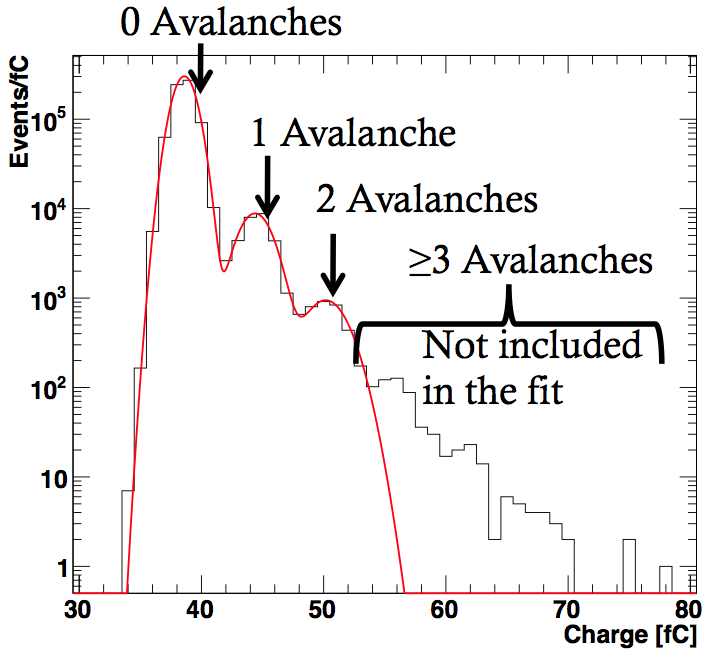
\includegraphics[width=\textwidth]{Figures/kuensken/gainDetermination.png}
\caption{Dark noise spectrum of an SiPM. plotted in red is the fit that is used for gain determination \cite{kuenskenCalor}.}
\label{kuenskendarkNoise}
\end{minipage}
\end{figure}
Each data point represents the temperature on a PCB at a given time. Deviations stay within a range of 0.1\,$^\circ$C which corresponds to a change of 5.6\,mV in the bias voltage.

\subsubsection{Gain}
The gain determines the signal height that is produced by an SiPM and thus the measured charge. It is necessary to know the gain of an SiPM to determine the number of photons that triggered the SiPM and get a measure of the deposited energy in the detector. HO uses two ways of determining the gain.
The first is to use the dark noise spectrum of an SiPM that develops due to thermal excitation of electrons in the active volume of an SiPM cell and the subsequent breakdown of that cell. A gauss fit is performed to the pedestal peak and the peaks of one and two avalanches. From the distance of the peak positions the gain is calculated. This method is known as the PED method. An example dark noise spectrum together with an applied fit is shown in Fig. \ref{kuenskendarkNoise}.
\begin{figure}[htbp]
\centering
\begin{minipage}[t]{0.475\textwidth}
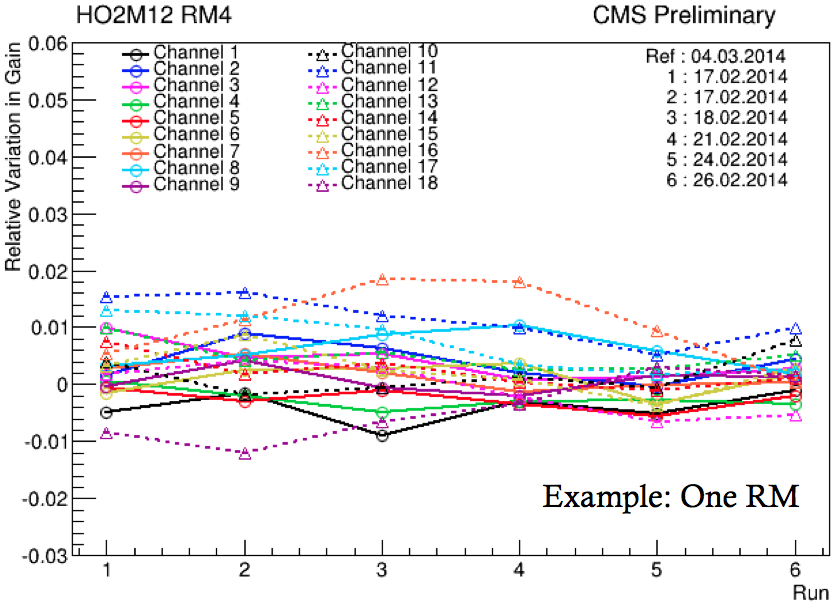
\includegraphics[width=\textwidth]{Figures/kuensken/gainOverTime.png}
\caption{Relative gain variation against time using the dark noise spectrum for gain determination \cite{kuenskenCalor}.}
\label{kuenskengainVsTime}
\end{minipage}
\hspace{0.5cm}
\begin{minipage}[t]{0.475\textwidth}
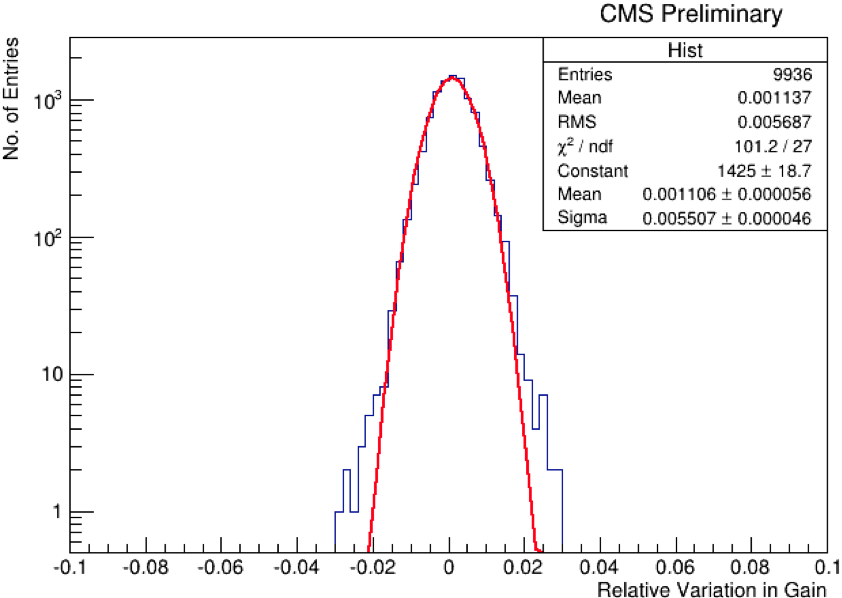
\includegraphics[width=\textwidth]{Figures/kuensken/gainTotal.png}
\caption{Histogram of all measured relative gain variations using the dark noise spectrum. The measurements were performed during the same period as is shown in Fig. \ref{kuenskengainVsTime} \cite{kuenskenCalor}.}
\label{kuenskengainHist}
\end{minipage}
\end{figure}
The second method uses short light pulses from an LED onto the SiPMs. When the light pulses contain not too many photons, the resulting signal distribution has a mean of
\begin{equation}
\text{m}=\text{N}\times \text{gain}
\end{equation}
and a width of
\begin{equation}
\sigma=\sqrt{\text{N}}\times \text{gain}
\end{equation}
assuming Poisson statistics for the uncertainty of the number of photons. Dividing the square of the measured width of the distribution by the measured mean, one obtains the gain of an SiPM as
\begin{equation}
\frac{\sigma^2}{\text{m}}=\frac{\text{N}\times \text{gain}^2}{\text{N}\times \text{gain}}=\text{gain.}
\end{equation}
This is called the LED method.
Before reviewing the comparability of the different methods it is necessesary to assure that the means of gain determination are stable. The relative gain variation versus time using the dark noise
spectrum is depicted in Fig. \ref{kuenskengainVsTime}. For a single PCB the relative gain variation is constant within 2\,\%. A histogram showing the relative gain variations for the same period for all installed SiPMs is plotted in Fig. \ref{kuenskengainHist}. The largest variations are within 3\,\%. The correlation between the two possibilities of determining the gain is printed in Fig. \ref{kuenskengainCorr}.
\begin{figure}[htbp]
\centering
\begin{minipage}[b]{0.475\textwidth}
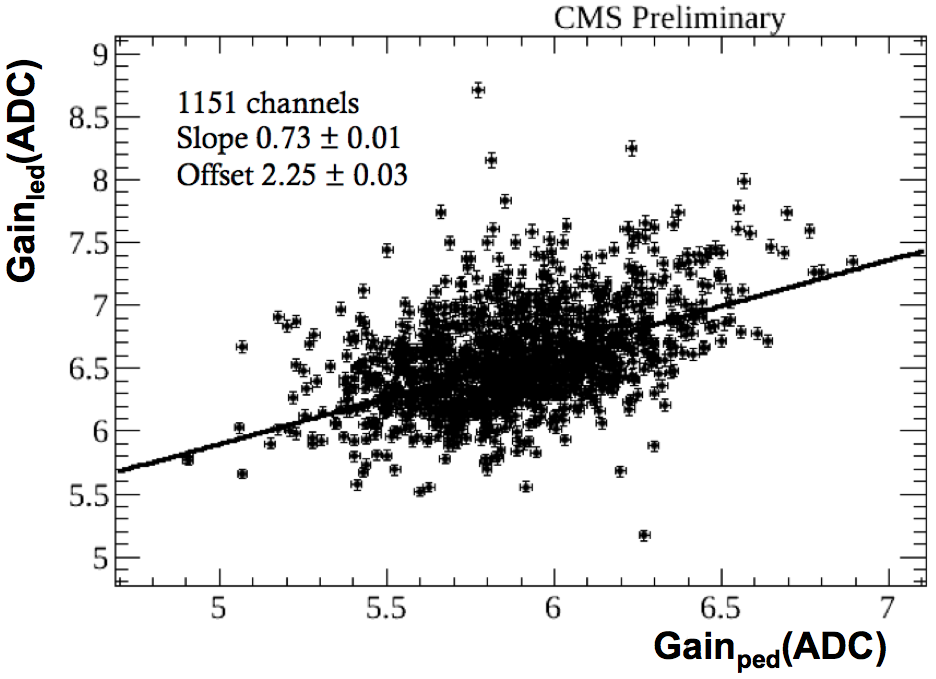
\includegraphics[width=\textwidth]{Figures/kuensken/gainCorrelation.png}
\end{minipage}
\hspace{0.5cm}
\begin{minipage}[b]{0.475\textwidth}
\caption{Correlation between the two methods for determining the gain. The values are distributed close to the design gain of 6\,ADC. Presented in \cite{kuenskenCalor}.}
\label{kuenskengainCorr}
\end{minipage}
\end{figure}
The plot shows that the measured gain values are centered around a specific value and no large deviation are found. However, it can be noticed that the mean gain value for the LED method is systematically shifted with respect to the results from the dark noise spectrum. This shift can be explained by the fact that the spectrum measured with the LED method is not exactly gaussian. This results in a shift towards higher gain values for this method. Once this offset has been characterized it would be possible to correct for it.

\subsubsection{Breakdown voltage}
The gain of an SiPM depends on the voltage difference between the applied voltage and the breakdown voltage of the device. It is therefore necessary to have reliable means of determining the breakdown voltage of an SiPM in order to keep the gain stable. In HO there are two ways of measuring the breakdown voltage. The first one exploits again the dark noise spectrum of an SiPM. By measuring the gain using the dark noise spectrum for different bias voltages the gain versus the bias voltage is plotted. It is then possible to fit a straight line to the distribution and extrapolate to a gain of zero pointing to the breakdown voltage. This is referred to as the PED method. The second way of breakdown voltage determination uses an LED again. The collected charge is measured for different bias voltages and then the relative derivative $\frac{\text{dS}}{\text{SdV}}$ is calculated. The resulting distribution has a maximum where the measured signal changes most with the bias voltage which is taken as the bias voltage. This method is referred to as the LED method.
\begin{figure}[htbp]
\centering
%\begin{minipage}[t]{0.475\textwidth}
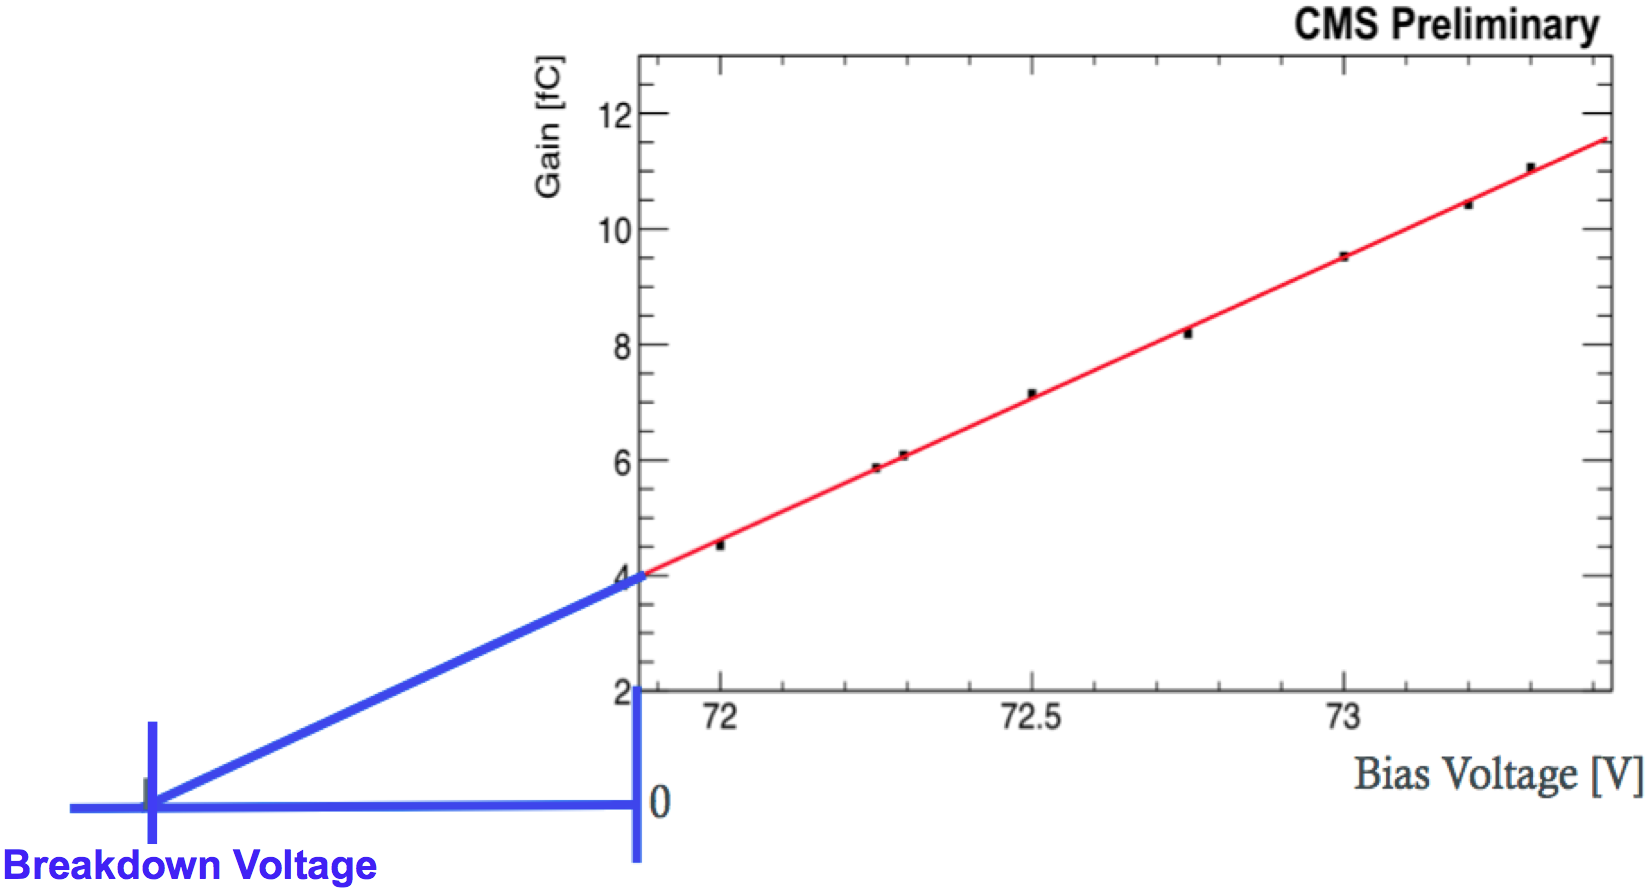
\includegraphics[width=0.9\textwidth]{Figures/kuensken/bvPedDetermination.png}
\caption{Determination of the breakdown voltage of an SiPM using the gain from dark noise spectrums measured at different bias voltages. Shown in \cite{kuenskenCalor}.}
\label{kuenskenbvPed}
%\end{minipage}
%\hspace{0.5cm}
\end{figure}
The determination of the breakdown voltage using the dark noise spectrum and the LED spectrum are shown in Fig. \ref{kuenskenbvPed} and Fig. \ref{kuenskenbvLed}, respectively.
\begin{figure}[htbp]
\centering
\begin{minipage}[htbp]{0.39\textwidth}
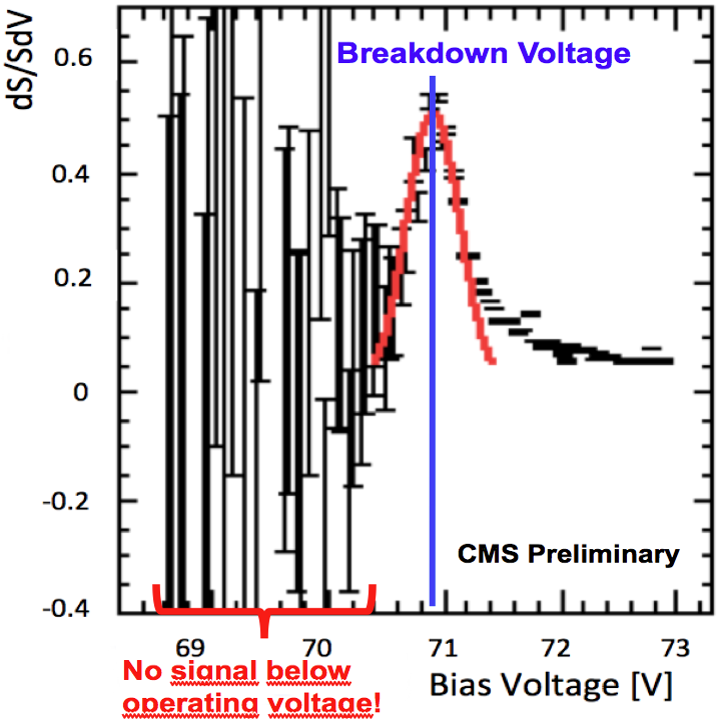
\includegraphics[width=\textwidth]{Figures/kuensken/bvLedScaled.png}
\caption{Breakdown voltage determination using the relative derivative of LED spectra measured at different bias voltages. Image from \cite{kuenskenCalor}.}
\label{kuenskenbvLed}
\end{minipage}
\hspace{0.5cm}
\begin{minipage}[htbp]{0.56\textwidth}
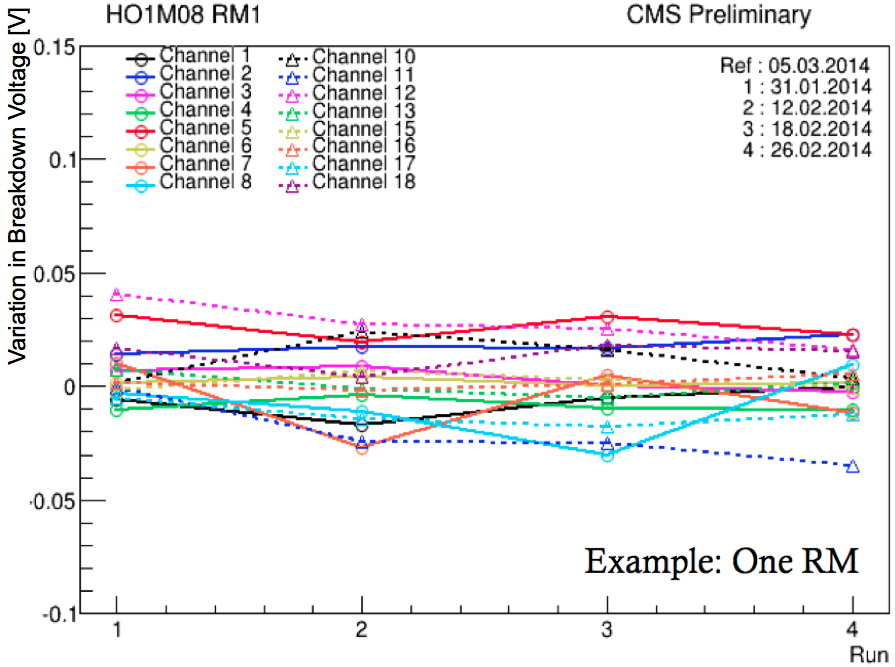
\includegraphics[width=\textwidth]{Figures/kuensken/bvOverTime.png}
\caption{Distribution of breakdown voltage measured with the PED method. Taken from \cite{kuenskenCalor}.}
\label{kuenskenbvVsTime}
\end{minipage}
\end{figure}
The variation of the breakdown voltage for a set of SiPMs on a single mounting board versus time is presented in Fig. \ref{kuenskenbvVsTime}. The employed method for the determination of the breakdown voltage is the PED method. The plot shows that the variation of the breakdown voltage stays within 50\,mV. The correlation between the two methods is shown in Fig. \ref{kuenskenbvCorr}. The data points align along a straight line which demonstrates a well defined linear relation between the values of the two methods. The spread of the breakdown voltages is due to the fact that not all devices have the same breakdown voltage. However, it can be noted that there is an offset between the two methods which shows itself in the y-intercept. This stems from the slightly different criteria for the determination of the breakdown voltage. Once the offset is determined the breakdown voltages can be corrected.
\begin{figure}
\centering
\begin{minipage}[htbp]{0.475\textwidth}
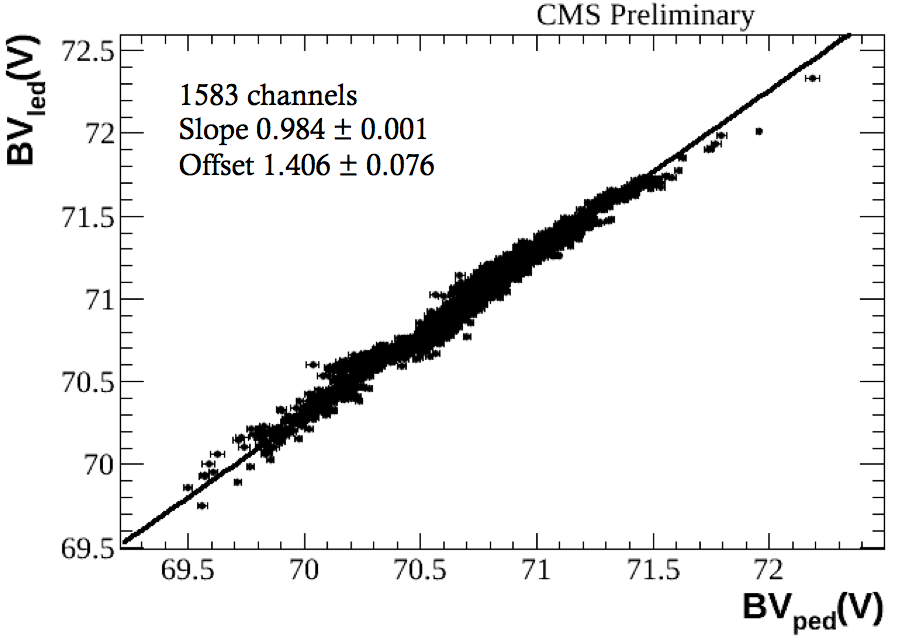
\includegraphics[width=\textwidth]{Figures/kuensken/bvCorrelation.png}
\end{minipage}
\hspace{0.5cm}
\begin{minipage}[htbp]{0.475\textwidth}
\caption{Correlation of the different methods for measuring the breakdown voltage. Taken from \cite{kuenskenCalor}.}
\label{kuenskenbvCorr}
\end{minipage}
\end{figure}
\newline
The HO system was successfully upgraded to SiPM readout during Long Shutdown 1, operation conditions (SiPM gain and breakdown voltage e.g.) are well understood and under control.
Studies on the muon detection capabilities of the already upgraded detector areas are now possible.
% i m a g e   c o m a n d:
% usage: \image[pos]{size}{file}{caption}
% => label = "image:<file>"
% default of [pos] is [!htb]
\newcommand{\image}[4][!htb]{
  \begin{figure}[#1]
    \centering
    \includegraphics[#2]{#3}
    \caption{#4}
    \label{image:#3}
  \end{figure}
}
%
% d o u b l e i m a g e   c o m a n d:
% usage: \doubleimage[pos]{size1}{file1}{subcaption1}{size2}{file2}{subcaption2}{caption}{hspace}
% => label = "image:<file1>"
% default of [pos] is [!htb]
\newcommand{\doubleimage}[9][!htb]{
  \begin{figure}[#1]
    \centering
    \subfloat[#4]{\includegraphics[#2]{#3}}
    \hspace{#9}
    \subfloat[#7]{\includegraphics[#5]{#6}}
    \caption{#8}
    \label{image:#3}
  \end{figure}
}
\newpage
\section{Prototype module}
\label{section:simon}
In this chapter, results of a MTT prototype detector with a $100 \times 100 \times 5 \,\text{mm}^3$ scintillator tile and dual SiPM readout are presented. A detailed description of the prototype and the experimental setup is given in Section \ref{section:simon/setup}. Section \ref{section:simon/optimization} shows results of comparisons between different system parameters. The performance of an optimized prototype is evaluated in Section \ref{section:simon/performance} and part \ref{section:simon/outlook} gives a brief outlook on research goals of the near future.
%
\subsection{Experimental setup}
\label{section:simon/setup}
The studies presented in this node were all performed with the prototype shown in Figure \ref{image:Figures/simon/setup/M7_tp.png} (without top cover).\image{width = .5\textwidth}{Figures/simon/setup/M7_tp.png}{The $10 \times 10 \,\text{cm}^2$ prototype for the MTT system} The module consists of a fast $100 \times 100 \times 5 \,\text{mm}^3$ wide organic scintillator of type \emph{BC-404} by Saint-Gobain and is read out by two silicon photomultipliers of type \emph{S10362-33-100C} by Hamamatsu. The concept of a dual SiPM readout was chosen because of the high noise rate of SiPMs. The frontend electronics offers three signal outputs: both amplified SiPM signals and the amplified analogue sum of both signals. Since the dark noise in both SiPMs is independent the sum signal provides a better signal to noise ratio.

The BC-404 scintillator was chosen for its fast timing capabilities (decay time of $1.8\,\text{ns}$) and the highest light output in the BC-400 series with the drawback of the shortest light attenuation length of $140\,\text{cm}$. The emission spectrum of the scintillator shown in Figure \ref{image:Figures/simon/setup/BC404-Spektrum.png} a) has its maximum at $\lambda_\text{max} = 408\,\text{nm}$ and is limited roughly in the range between $380\,\text{nm}$ and $500\,\text{nm}$. The scintillator is wrapped in PTFE tape (Polytetrafluoroethylene, widely known by DuPont's brand name \emph{Teflon}) which is a diffuse reflector.

The S10362-33-100C SiPMs have an active area of $3 \times 3\,\text{mm}^2$ with a pixel pitch of $100\,\mu\text{m}$ which lead to a total pixel number of $300 \times 300$. Figure \ref{image:Figures/simon/setup/BC404-Spektrum.png} b) shows the emission spectrum of the familiar SiPM type S10362-33-050C, which has the same active area with smaller pixel pitch. The figure clearly shows that the detection efficiency of the S10362 series is highest for wavelengths between $400\,\text{nm}$ and $500\,\text{nm}$, which makes them a good match for the chosen scintillator BC-404. Dedicated investigations of Hamamatsu's SiPMs are presented in Chapter [REF THOMAS], the frontend electronics which amplifies the SiPM signals and regulates the bias voltages is described in Chapter [REF LARS].

\doubleimage
{width = .4\textwidth}{Figures/simon/setup/BC404-Spektrum.png}{Emission spectrum of BC-404 ((REF))}
{width = .4\textwidth}{Figures/simon/setup/S10362-33-Spektrum.png}{Detection efficiency of S10362-33-050C type SiPM ((REF))}
{The emission spectrum of Saint-Gobain scintillator BC-404 and spectral detection efficiency of Hamamatsu S10362-33-050C type SiPM match nicely}
{.07\textwidth}

The signal spectrum of the module, externally triggered with cosmic muons, is shown in Figure \ref{image:Figures/simon/setup/Wrapping2_PULSE_S_FIT.pdf}. A small inefficiency is visible in the pedestal peak at about $40\,\text{mV}$ which is clearly separated from the landau shaped signal distribution with the most probable value around $230\,\text{mV}$. The second peak at roughly $600\,\text{mV}$ is due to a saturation effect of the preamplifiers.
\image{width = .6\textwidth}{Figures/simon/setup/Wrapping2_PULSE_S_FIT.pdf}{Pulse spectrum of the prototype module for cosmic muons}

All measurements presented in the next chapter have been performed with cosmic muons, triggered by the coincidence of two scintillators read out with photomultiplier tubes. For older measurements the pulses were evaluated with a CAEN V965 12-bit QDC and later fully digitized with a CAEN VX1721 8-bit FADC, which allowed the calculation of the exact pulse height over baseline for every event.
\subsection{Parameter optimization}
\label{section:simon/optimization}
To achieve the best possible light yield and to gain a deeper understanding of the prototype several parameters have been investigated separately, some of which are presented in this section. To compare different setups, each configuration has been tested with 3000 -- 5000 cosmics and a landau fit was performed on the resulting QDC or FADC spectrum (as previously shown in Figure \ref{image:Figures/simon/setup/Wrapping2_PULSE_S_FIT.pdf}). The most probable values (MPV) of these fits are used as a quality criteria for the given configuration and presented for all three signal outputs (SiPM A, analogue sum, SiPM B) in bar charts.
%
\subsubsection{Wrapping material}
A very important component of the detector is the reflective wrapping material of the scintillator since it directly effects the light yield. Therefore aluminium foil has been tested as a specular reflector and compared to a multi layer wrapping of PTFE tape as a diffuse reflector. The result is shown in Figure \ref{image:Figures/simon/optimization/VergleichAluTape_QDC.pdf}. Wrapping the scintillator with PTFE tape leads to a significant increase in the signal height of about $70\,\%$ -- $90\,\%$. Therefore, all further measurements have been performed with PTFE tape as reflector, applied in three layers.
\image{width = .6\textwidth}{Figures/simon/optimization/VergleichAluTape_QDC.pdf}{Comparison between aluminium foil and PTFE tape as reflective wrapping material}
%
\subsubsection{Scintillator thickness}
Since the CMS detector is by definition a very compact experiment, one of the goals for the MTT system is to provide a thin detector layer. Therefore the effect of the scintillator thickness is of interest and a comparison between a $5\,\text{mm}$ and a $10\,\text{mm}$ thick scintillator has been made. The results of this comparison are depicted in Figure \ref{image:Figures/simon/optimization/VergleichDicke_QDC.pdf}. The light yield drops when changing the $10\,\text{mm}$ scintillator to a $5\,\text{mm}$ thick one, but not as much as one would expect geometrically. The signal loss lies in the region of $10\,\%$ -- $15\,\%$, which is an acceptable trade off for a $50\,\%$ decrease in detector thickness. Therefore, all further measurements have been performed with a $5\,\text{mm}$ thick scintillator.
\image{width = .6\textwidth}{Figures/simon/optimization/VergleichDicke_QDC.pdf}{Comparison between a $5\,\text{mm}$ and a $10\,\text{mm}$ thick scintillator}
%
\subsubsection{Coupling between SiPM and scintillator}
\doubleimage 
{width = .4\textwidth}{Figures/simon/optimization/coupling/grease.jpg}{Silicone grease: Saint-Gobain BC-630}
{width = .4\textwidth}{Figures/simon/optimization/coupling/grease_dry.JPG}{Dried BC-630}
{The silicone grease BC-630 by Saint-Gobain dries within a couple of days}
{.07\textwidth}
One of the most critical points of scintillator based detectors is the optical coupling between the scintillator and the light detector. In the first MTT prototypes, optical coupling has been done with the \emph{BC-630 optical grease} by Saint-Gobain which is shown in Figure \ref{image:Figures/simon/optimization/coupling/grease.jpg} (a). After applying the grease, the detector signals dropped significantly within a week's time, which can be explained with Figure \ref{image:Figures/simon/optimization/coupling/grease.jpg} (b). The figure shows the scintillator edge to which the grease had been applied. One can clearly make out that the grease has dried out or partially evaporated on the surface and therefore the optical connection between the SiPM and the scintillator suffered significantly. With this result, the BC-630 can obviously not be considered as a long-term solution for the MTT system. Therefore two other methods of coupling the SiPM to the scintillator have been tested: The silicone gel \emph{RTV 6151} by GE Silicones and silicone rubber pads made out of \emph{RT 604} by ELASTOSIL. Pictures of both options are depicted in Figure \ref{image:Figures/simon/optimization/coupling/silicone_gel.jpeg}.
\doubleimage
{width = .4\textwidth}{Figures/simon/optimization/coupling/silicone_gel.jpeg}{Silicone gel: GE Silicones RTV 6151}
{width = .4\textwidth}{Figures/simon/optimization/coupling/silicone_rubber.jpg}{Silicone rubber: ELASTOSIL RT 604}
{The two component silicone gel RTV 6151 by GE Silicones and silicone rubber pads made out of ELASTOSIL RT 604 were tested as alternatives}
{.07\textwidth}
Both alternatives are silicone based and mixed of two components. Remaining air pockets are removed from the mixture under a vacuum bell jar. The RTV 6156 has been applied directly to the scintillator, cured in the assembled module and therefore adopted perfectly to the SiPM geometry. On the other hand, a $1\,\text{mm}$ thick layer of RT 604 had been cast and hardend on a glass surface from which small pads can be cut out. The idea to produce these pads is inspired by conventional photo multiplier tubes, where similar pads have been used for many years as optical coupling between scintillators and light guides. The great advantage of these pads is their reusability and the simple detector assembly.

Measurements with all these coupling methods including one without any additional optical layer have been performed with cosmic muons. The results are shown in Figure \ref{image:Figures/simon/optimization/VergleichKopplungen_PULSE.pdf}. The importance of an optical medium is clearly visible, all three methods lead to an significant increase of light yield. Out of the three substances the BC-630 provided the best result, even though it cannot be used long term as described above. The other two methods are slightly but not significantly worse. The RTV 6151 should be used as the long term solution for the MTT system. However, for testing purposes the RT 604 pads have been chosen for all following measurements due to their flexibility and ease of use. 
\image{width = .6\textwidth}{Figures/simon/optimization/VergleichKopplungen_PULSE.pdf}{Comparison between different optical couplings between the SiPMs and the scintillator}
%
%
\subsubsection{Coupling reproducibility}
\label{section:simon/optimization/recoupling}
Because the prototype module often had to be reassembled for different setups, it is important to investigate how this effects the detector signals. For this purpose the frontend electronics have been separated from the module and reassembled with new silicone pads four times. The results depicted in Figure \ref{image:Figures/simon/optimization/VergleichZusammenbau_PULSE.pdf} show uncritical fluctuations in the region of $\leq 5\,\%$ (RMS). 
\image{width = .6\textwidth}{Figures/simon/optimization/VergleichZusammenbau_PULSE.pdf}{Effect of reassembly of the module using silicone rubber}
%
\subsubsection{Wrapping reproducibility}
\label{section:simon/optimization/rewrapping}
Similar to the investigation of the coupling reproducibility, the wrapping of the scintillator with PTFE tape has been tested by means of rewrapping the whole scintillator four times. In addition a new wrapping technique with particular attention to the scintillator edges and the reduction of possible air pockets has been applied. The results are shown in Figure \ref{image:Figures/simon/optimization/VergleichWrapping_PULSE.pdf}. The new wrapping technique clearly increases the light yield, which was up to $30\,\%$ lower with the old wrapping. The fluctuations of the signal height when rewrapping the scintillator are about $8\,\%$ (RMS).
\image{width = .6\textwidth}{Figures/simon/optimization/VergleichWrapping_PULSE.pdf}{Effect of rewrapping the scintillator tile with PTFE tape}
\subsection{Prototype performance}
\label{section:simon/performance}
To determine the usefulness of the MTT prototype module as a muon trigger calculations of the signal purity and the detection efficiency are presented in this chapter.
\subsubsection{Signal purity}
In addition to the detection efficiency, which is the most important attribute of a trigger detector, the signal purity is of great importance. Since all prototype studies have been done with cosmic muons the purity is also calculated with respect to cosmics. Purity is hereby defined as the probability, that a detector pulse over a certain threshold has been triggered by a real (cosmic) muon passing the detector and not due to high SiPM noise. To calculate this purity one needs to know the fraction of muon pulses and SiPM noise pulses for any given threshold. To get these fractions two measurements of pulse rate over threshold have been performed. First pulses of the whole prototype module were recorded, including noise and muon pulses (total rate). Secondly the signal rate of the same module was recorded without the scintillator and thereby eliminating the muon signals (noise rate). The purity can then be calculated by:
\begin{equation}
 \text{purity} = \frac{\text{muon rate}}{\text{total rate}} = \frac{\text{total rate} - \text{noise rate}}{\text{total rate}}
\end{equation}
The result of these measurements and the calculated purity for the sum signal are shown in Figure \ref{image:Figures/simon/performance/purity.png}. With a trigger threshold of around $40\,\text{mV}$ a signal purity of more than $99.9\,\%$ is reached.
\image{width = .6\textwidth}{Figures/simon/performance/purity.png}{Purity of the prototype sum signals over threshold}
%
\subsubsection{Detector efficiency}
When building a trigger system, a high detection efficiency is of great importance. Therefore the efficiency of the MTT prototype is determined as a function of the potential trigger threshold from the combination of all measurements from Section \ref{section:simon/optimization/recoupling} (recoupling the SiPMs to the scintillator) and Section \ref{section:simon/optimization/rewrapping} (rewrapping the scintillator). The calculation and error estimation follows the guidelines given in ((REF)). The result is shown in Figure \ref{image:Figures/simon/performance/KombiEffBayes_Square_Summe.png}. Figure \ref{image:Figures/simon/performance/KombiEffBayes_Square_Summe.png} (a) shows the combined efficiency plotted against the full dynamic range of the module and Figure \ref{image:Figures/simon/performance/KombiEffBayes_Square_Summe.png} (b) is a magnification of the interesting region. The red shaded region in \ref{image:Figures/simon/performance/KombiEffBayes_Square_Summe.png} (b) includes all efficiency lines calculated from each measurement of Section \ref{section:simon/optimization/rewrapping} and the green shaded area corresponds to the efficiency lines calculated from the measurements of Section \ref{section:simon/optimization/recoupling}. Therefore the shaded areas provide information about the systematic fluctuations of the efficiency due to the wrapping of the scintillator and the assembly of the module. The data points represent the combined efficiency for all measurements. For a trigger threshold between $50\,\text{mV}$ and $100\,\text{mV}$ the efficiency is compatible with $99.5\,\%$. For single thresholds the efficiency $\epsilon$ and its uncertainty can be extracted, for instance for $z = 65\,\text{mV}$:
\begin{equation}
 \epsilon(z = 65\,\text{mV}) = (99.49\,\pm\,0.04)\,\%
\end{equation}
The width of the shaded areas can be used as an conservative estimate for the systematic uncertainties at the given point. For instance at $z = 65\,\text{mV}$:
\begin{equation}
 \Delta\epsilon(\text{wrapping}) = 0.24\,\%
\end{equation}
and
\begin{equation}
 \Delta\epsilon(\text{assembly}) = 0.16\,\%.
\end{equation}
\doubleimage
{width = .4\textwidth}{Figures/simon/performance/KombiEffBayes_Square_Summe.png}{Full dynamic range of the module}
{width = .4\textwidth}{Figures/simon/performance/AreaFill_Zoom_Square_Summe.png}{Systematic influences}
{Efficiency of the prototype detector over threshold for the sum signal, combined from several measurements}
{.07\textwidth}
\newpage
\subsection{Upcoming prototype studies}
\label{section:simon/outlook}
The presented studies show that the $100 \times 100 \times 5 \,\text{mm}^3$ MTT prototype can be used as a reliable muon detector. Further studies with this prototype will investigate the timing resolution of the module, which is an important attribute for a trigger detector. In addition the homogeneity of the signal height as well as the homogeneity of the timing resolution will be determined. Also Tyvek paper is being considered as an alternative for the PTFE tape as diffuse reflector.

Since the optimal granularity of a possible MTT system has yet do be identified by simulations, larger prototypes will be studied as well. Therefore prototypes with $300 \times 300 \times 5 \,\text{mm}^3$ scintillators have already been produced, some of which with integrated wavelength shifting fibres. All prototypes will be tested in a proton test beam at Forschungszentrum J\"ulich in September 2014. With the planned setup it will be possible to investigate how the average signal height, the detection efficiency and the timing resolution are distributed over the detector surface and how different fibre layouts compare to each other in the larger modules.

\subsection{Prototype Simulations}
\label{sec:prototypeSimulations}

\textbf{\underline{Signal Homogeneity across a Scintillator Tile}}

In this simulation the signal homogeneity across a scintillator tile was investigated, i.e. to what extend the number of photons that reach the photon detector depends on the position at which a minimum ionising particle (MIP) hits the scintillator tile. Four different set-ups have been simulated: 100$\times$100$\times$5$\,$mm$^3$ and 350$\times$350$\times$5$\,$mm$^3$ scintillator tiles (BC-408) with Teflon wrapping and readout via one pseudo-SiPM, which was either attached directly to the tile or by an embedded wavelength-shifting fibre (cf. figure\enspace\ref{fig:simulatedSetups}). In case of the wavelength-shifting fibre, the end inside the scintillator has been mirrored and a pseudo-SiPM has been placed at the other end. For each of the four set-ups, 100000 MIP muons have been simulated randomly distributed over the scintillator surface, to obtain reasonable statistics.

\begin{figure}[h]
  \centering
  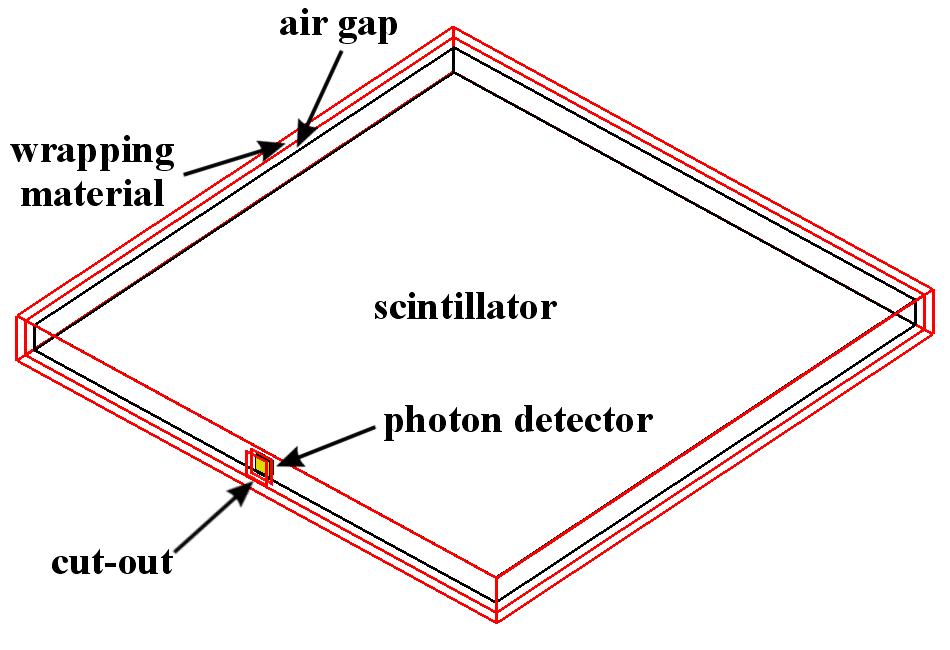
\includegraphics[width=8.9cm]{Figures/dietzlaursonn/wrapping.png}
  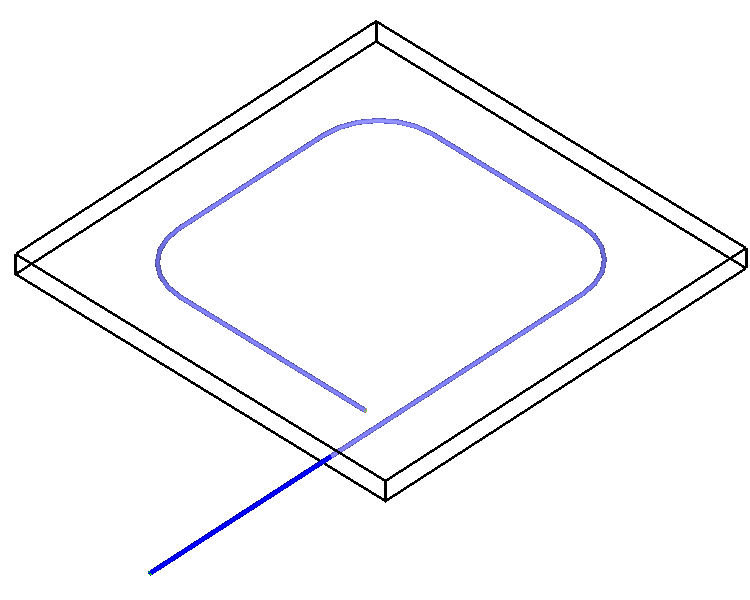
\includegraphics[width=7cm]{Figures/dietzlaursonn/fibre_sigma.png}
  \caption{\textbf{Left:} Set-up consisting of a wrapped scintillator tile with a photon detector. To make them visible, the dimensions of the wrapping as well as the free space between photon detector and wrapping, or scintillator and wrapping have been set to large values when generating the picture. \textbf{Right:} Relatively complex fibre set-up within and extending a scintillator tile.}
  \label{fig:simulatedSetups}
\end{figure}

In the following plots, the $x$- and $y$-axes represent the position at which the muons hit the scintillator tile. The colour-coded $z$-axis shows the most probable value (MPV) of the number of photons hitting the pseudo-SiPM. The MPV has been obtained by a fit of a Landau distribution to the distribution of the number of photons for the corresponding position bin. Since the energy deposition of a particle in thin layers of matter follows a landau distribution, no meaningful mean and standard deviation can be computed. As uncertainty on the number of photons, the uncertainty of the MPV of the fitted Landau distribution is taken. It is on average below 5\% across the tiles and below 10\% next to the SiPMs for direct readout.

Figure\enspace\ref{fig:signalHomogeneity} shows the signal homogeneity for all four simulated set-ups. For direct readout, the signal is relatively homogeneous over large areas and with values of MPV $\approx 550$ or MPV $\approx 50$ photons, depending on the dimensions of the scintillator tile. But in cases of muons that hit the scintillator tile in short distance to the pseudo-SiPM, the number of photons that reach the pseudo-SiPM increases dramatically by factors up to $\approx 5$ or $\approx 8$, depending on the dimensions of the scintillator tile. Such a signal inhomogeneity across the scintillator tile can be very problematic e.g. for the determination of the MIP muons. Additionally, depending on its number of pixels, an SiPM would probably be saturated and not able to detect multiple muon hits within a short time.

Using wavelength-shifting fibres to collect the scintillation light and to guide it to the pseudo-SiPM can significantly reduce this effect. This is illustrated in the bottom plots of figure\enspace\ref{fig:signalHomogeneity}. 
The signal is relatively homogeneous over the whole area with values of MPV $\approx 280$ or MPV $\approx 120$ photons, depending on the dimensions of the scintillator tile. In small distance to the fibre, the number of photons that reach the pseudo-SiPM increases, but only by $\approx 15\%$ or $\approx 60\%$, depending on the dimensions of the scintillator tile.

\begin{figure}[h]
\centering
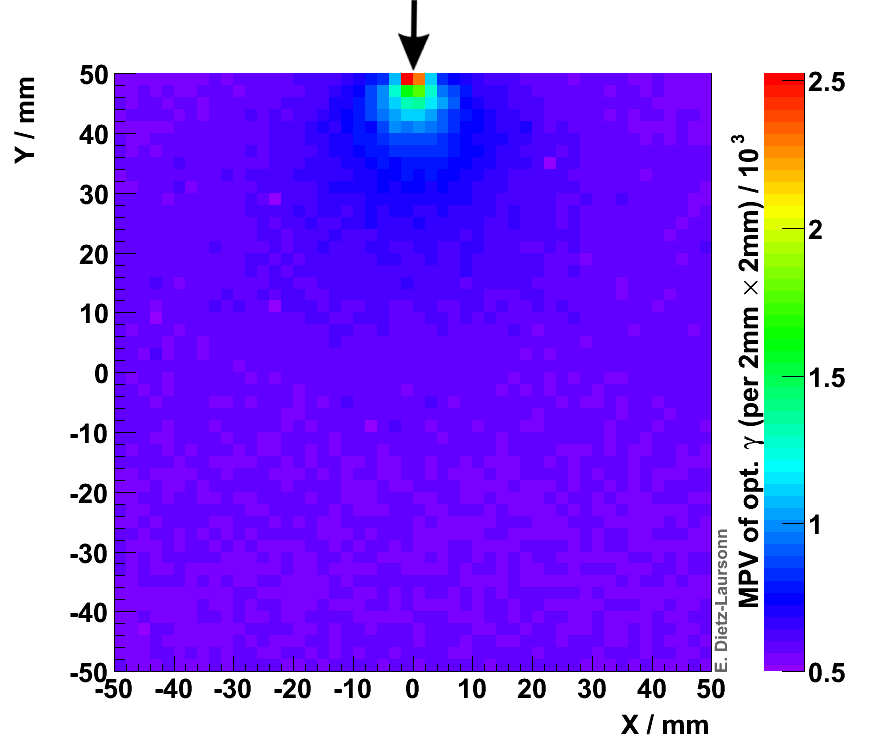
\includegraphics[width=7.9cm]{Figures/dietzlaursonn/101_100x5x100_Teflon__dataSim_opticalPhotons_on_SiPM_vs_hit_position.png}
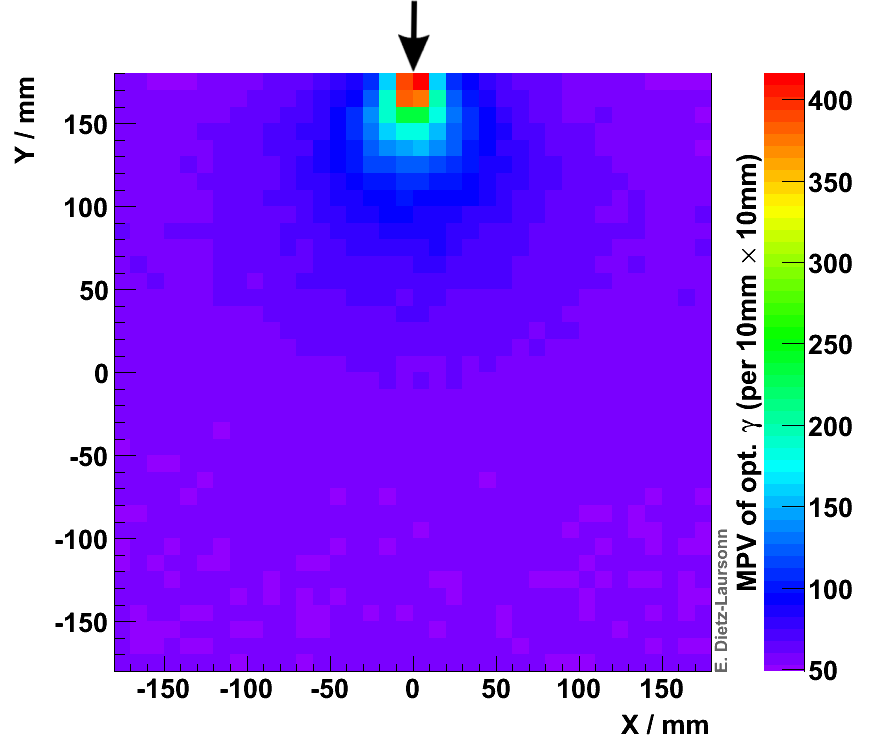
\includegraphics[width=7.9cm]{Figures/dietzlaursonn/101_350x5x350_Teflon__dataSim_opticalPhotons_on_SiPM_vs_hit_position.png}

\vspace{0.5cm}
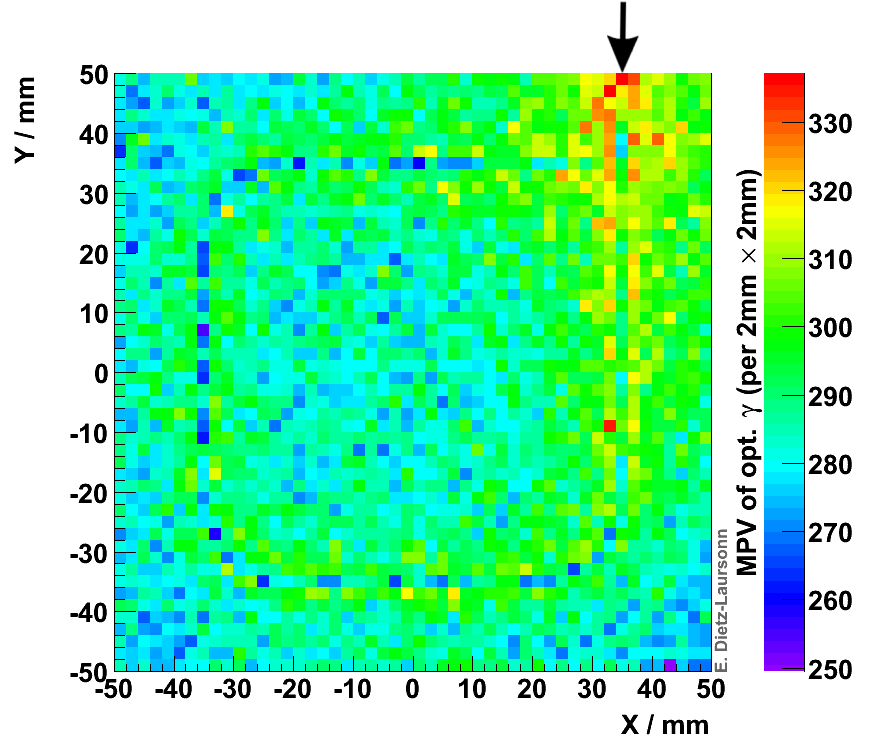
\includegraphics[width=7.9cm]{Figures/dietzlaursonn/411_100x5x100_Teflon__dataSim_opticalPhotons_on_SiPM_vs_hit_position.png}
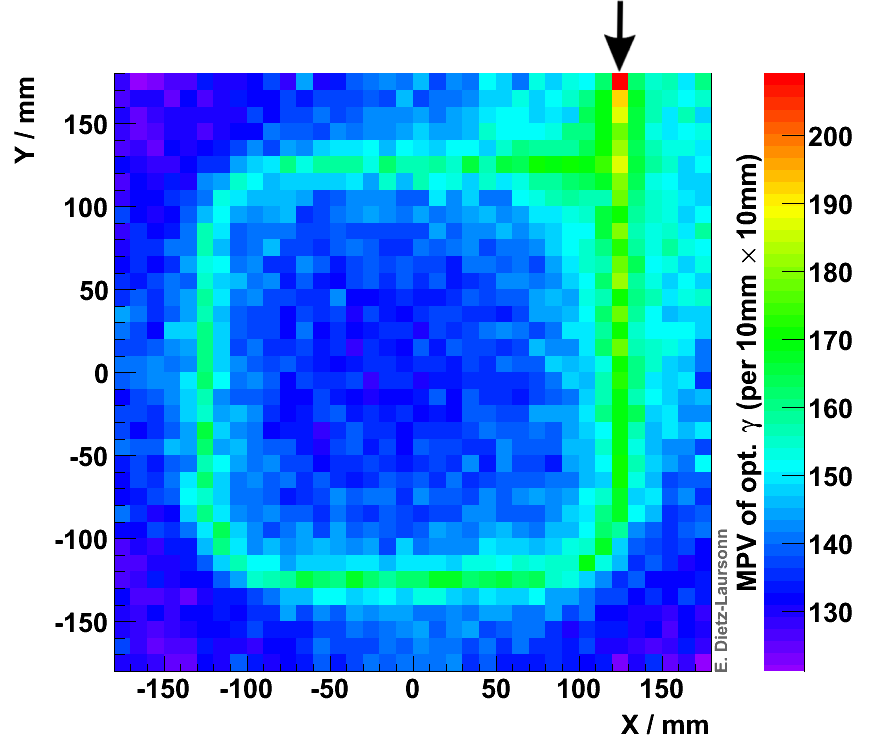
\includegraphics[width=7.9cm]{Figures/dietzlaursonn/411_350x5x350_Teflon__dataSim_opticalPhotons_on_SiPM_vs_hit_position.png}
\caption{Signal homogeneity for all four simulated set-ups: \textbf{Top-left:} 100$\times$100$\times$5$\,$mm$^3$ scintillator tile with direct readout, \textbf{Top-right:} 350$\times$350$\times$5$\,$mm$^3$ scintillator tile with direct readout, \textbf{Bottom-left:} 100$\times$100$\times$5$\,$mm$^3$ scintillator tile with fibre readout, \textbf{Bottom-right:} 350$\times$350$\times$5$\,$mm$^3$ scintillator tile with fibre readout. The arrows indicate the SiPM positions.}
\label{fig:signalHomogeneity}
\end{figure}




\textbf{\underline{Validation with hodoscope measurements}}

As validation, the results of the simulation have been compared to measurements that have been performed with a prototype detector tile within a hodoscope. The prototype detector tile consist of  a 100$\times$100$\times$5$\,$mm$^3$ scintillator tile (BC-408) with Teflon wrapping and two SiPMs. Both SiPMs are coupled to the scintillator tile at one of its thin surfaces, at a distance of 2$\,$cm with respect to the centre position. The data acquisition of the SiPM signal has been performed via a Charge-to-Digital-Converter.

The hodoscope consist of two layers of two vertical Silicon-Strip-Detectors each. They provide two positions (and thus the trajectory) of  cosmic muons and therefore allow the determination of the muon's hit position on the prototype detector tile, which is placed between the two hodoscope layers.

Up to now, 8436 cosmic muon tracks could be recorded and measured by the SiPMs.



In the following plots, the $x$- and $y$-axes again represent the position where the muons hit the scintillator tile. The uncertainties on the measured hit position on the scintillator tile are negligible in comparison to the used bin width. The relatively large bin width is due to the low statistics.
The colour-coded $z$-axis shows the difference between measured and simulated MPV. Since the measurement results in the MPV of the SiPM signal charge, only relative values can be compared. Therefore, the original MPV values have been scaled to the mean value of the marked comparison area and the resulting relative values were used to determine the difference between measurement and simulation. The uncertainties shown in the histograms are the propagated MPV uncertainties of the fitted Landau distributions for both, the simulation and the measurement.



\begin{figure}[h]
\centering
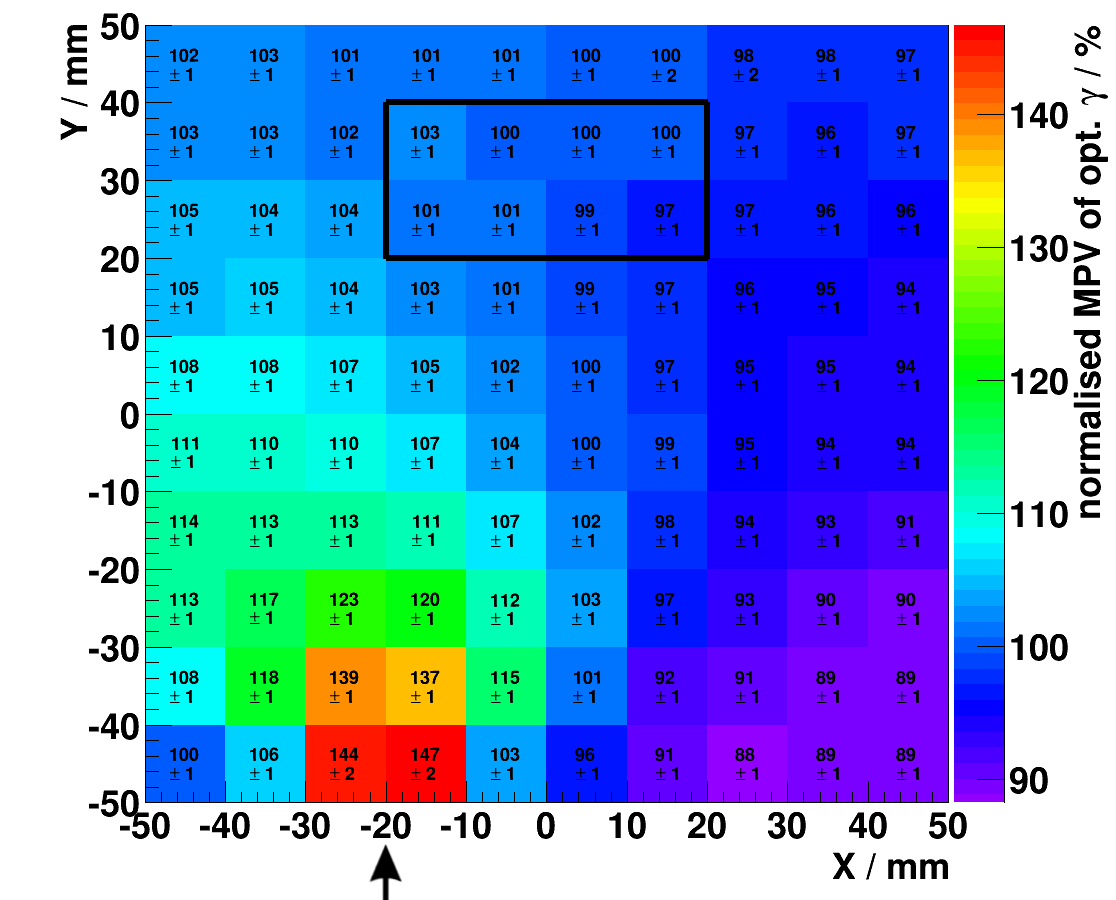
\includegraphics[width=7.9cm]{Figures/dietzlaursonn/comparison_sim_B_opticalCoupling_1_43_1cm.png}
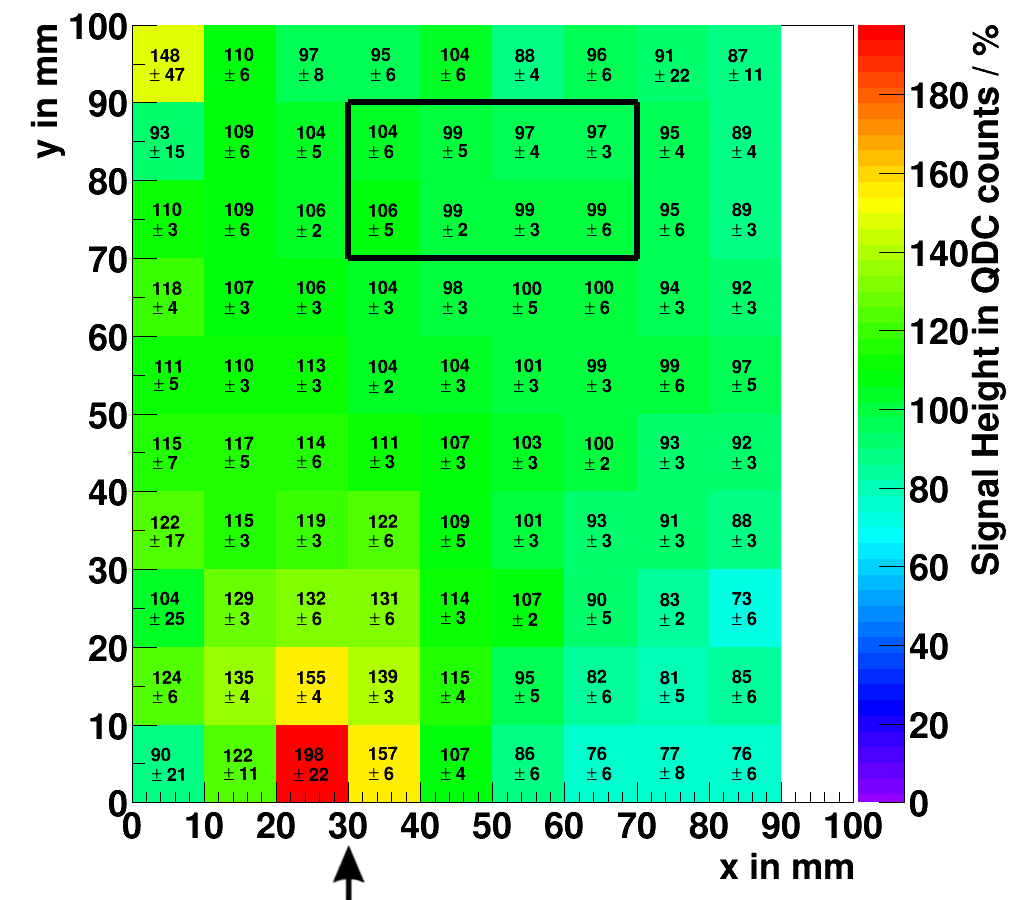
\includegraphics[width=7.9cm]{Figures/dietzlaursonn/comparison_meas_B_1cm.png}

\vspace{0.5cm}
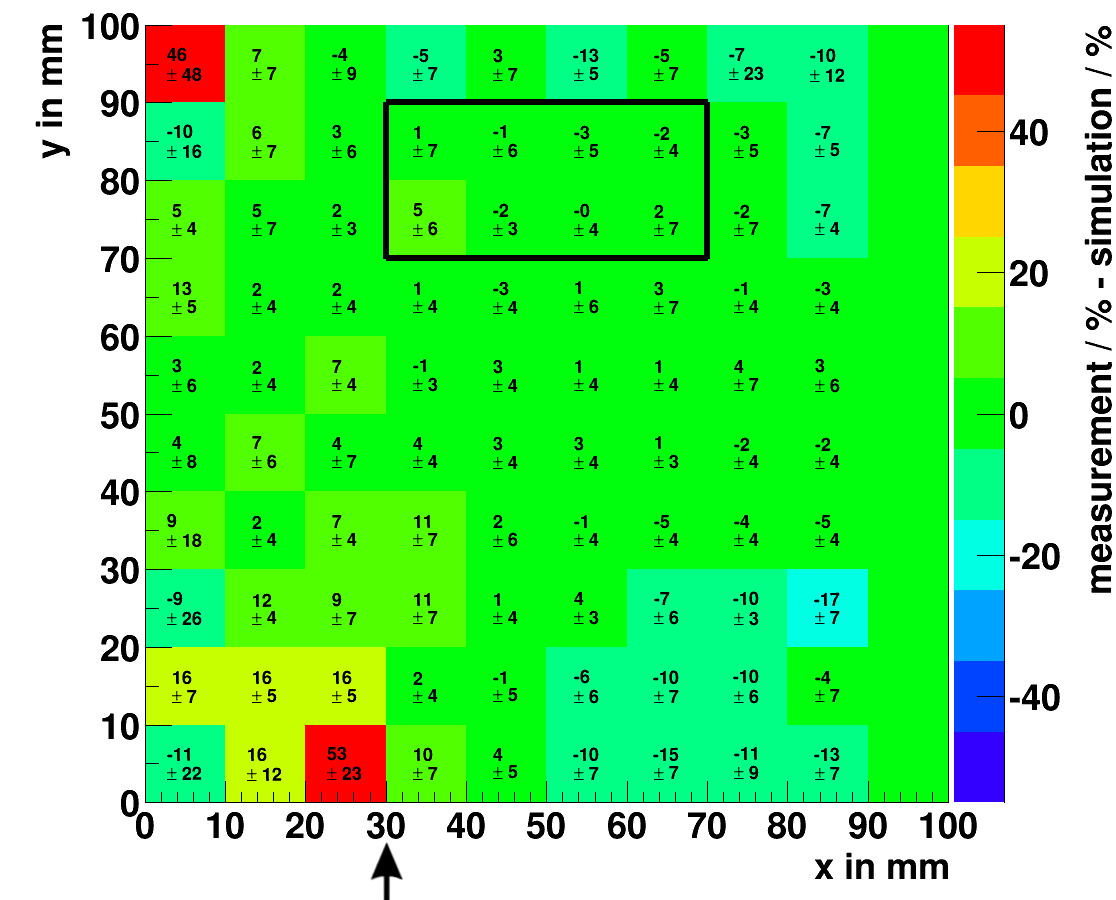
\includegraphics[width=8cm]{Figures/dietzlaursonn/comparison_diff_B_opticalCoupling_1_43_1cm.png}
\caption{Results for the comparison between measurement and simulation: \textbf{Top-left:} normalised simulation results, \textbf{Top-right:} normalised measurement results (the unfilled bins were caused by the geometry of the hodoscope), \textbf{Bottom:} the difference between simulation and measurement. The arrows indicate the SiPM position and the results have been been scaled to the mean value of the marked comparison area.}
\label{fig:comparison}
\end{figure}



Figure\enspace\ref{fig:comparison} illustrates the scaled results of the simulation and the measurement as well as the difference between them. Again, the signal is relatively homogeneous over large areas and dramatically increases next to the SiPM position. The comparison shows, that the relative distribution of simulation and measurement are in very good agreement and the difference is compatible with 0 over a large area, when considering the uncertainties. As repeating the measurement after reassembling the detector reproduces the MPV values with 10\% accuracy, which is caused by the limited reproducibility of the optical coupling between scintillator tile and SiPM, the achieved agreement between simulation and measurement is an excellent result.


\documentclass[]{article}
\usepackage{amsmath}
\usepackage{graphicx}
\begin{document}

\newpage
\section{Frontend Electronics}

This chapter serves as a technical documentation of the electronics currently in use and under development for MTT.

\subsection{APDPI}

The Avalanche Photodiode Power Interface (APDPI) is a standard NIM module that supplies power for the SiPMs, amplifier circuits and logic of the frontend electronics.
Figure \ref{APDPI_front} shows the front panel of an APDPI module: On the top there is a DSUB-9 connector consisting of a VBIAS, V+, V-, GND, RTX+ and RTX- output.
Below the connector there are two switches BIAS and POWER and again below that a USB B plug.

The $+12\,\text{V}$ line of the NIM backend is fed to a DC-DC converter that is adjustable via a potentiometer located next to the converter.
The converter takes $10.8\,\text{V} .. 13.2\,\text{V}$ and outputs $0\,\text{V} .. 180\,\text{V}@15\,\text{mA}$ to the VBIAS line. The BIAS switch is located directly below the
DSUB-9 connector and switches VBIAS on and off. The typical VBIAS voltage currently used is $82\,\text{V}$.

V+ and V- supply a $\pm3.3\,\text{V}@1\text{A}$ power source respectively for the amplifier and logic circuits of the frontend electronics. There are two voltage regulators 
which use the $\pm6\,\text{V}$ lines of the NIM backend to generate the $\pm3.3\,\text{V}$ outputs. Below the VBIAS switch there is also a POWER switch located for V+ and V-.

GND is the reference potential for VBIAS as well as for V+ and V-. It uses the ground line of the NIM backend and is also connected to the casing of the 
module to reduce noise.

RTX+ and RTX- are the differential EIA-485 compliant outputs used for communication with and slow control of the frontend electronics. The EIA-485 (or RS-485) 
defines a physical layer that uses a differential signal for communcation thus providing a stable signal over distances of up to $1.2\,\text{km}$. The data link layer is 
compliant to the microcontroller friendly Universal Synchronous/Asynchronous Receiver Transmitter (USART) which simplifies the whole commucation chain in hardware. 
A computer can be connected to the APDPI via a USB B plug located beneath the POWER switch. The USB signal is mapped to USART by a \emph{FT232RL} 
chip and again converted to RS-485 by a \emph{MAX3086E} chip thus the slow control can be accessed with a simple 
FTDI serial driver.
The \emph{MAX3086E} transceiver provides a half duplex communication interface meaning that the driver uses the same data lines to transmit and receive data.

	\begin{figure}[t]
		\centering
			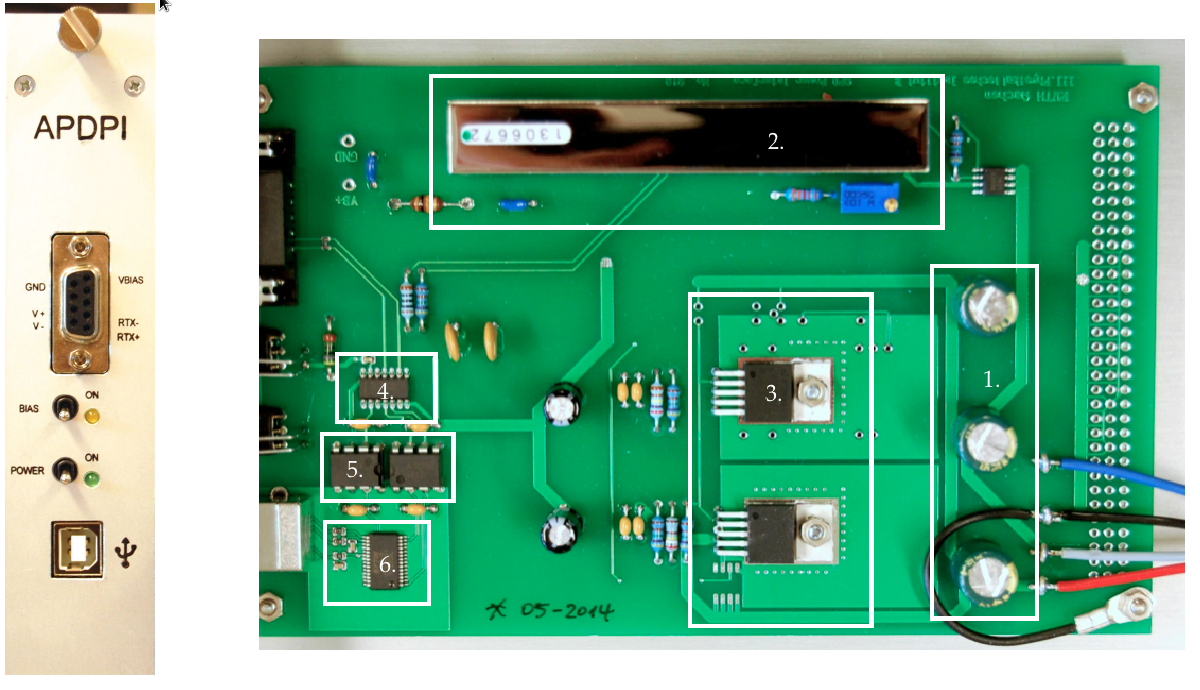
\includegraphics[width=1.0\textwidth]{Figures/weinstock/apdpi.png}
		\caption{\textbf{Left:} Front plate of an APDPI. \textbf{Right:} APDPI circuit: 1. $470\,\mu \text{F}$ bypass capacitors for the $\pm6\,\text{V}$ and $12\,\text{V}$ 
												   NIM lines;
												2. DC-DC converter and regulation potentiometer;
												3. $\pm3.3\,\text{V}$ voltage regulators with heat sink area;
												4. MAX3086E RS-485 to UART converter.
												5. Opto-isolators for electrical isolation of the FT232RL circuit. This circuit runs
												at $5\,\text{V}$ provided by the USB host;
												6. FT232RL UART to USB converter.}
		\label{APDPI_front}
	\end{figure}	

\subsubsection{SiPM Bus}

The SiPM Bus defines the application layer for the serial communication with the frontend electronics. The bus is host driven, so the bus master has to query for data from the slaves.
To ensure the correct understanding of the sent commands each individual byte is echoed by the slave and should be checked. To start the communication the bus master sends the start
delimiter character '$<$' (ASCII \verb|0x3C|) and claims the bus (start delimiter will not be echoed). Any further try to claim the bus will fail because the bus is now busy. 
The start delimiter then is followed by a unique 8 bit slave address which is echoed by the slave. The slave is now addressed and is ready to receive commands. For a complete list of
implemented commands and a short description see table \ref{sipm_bus_table}. Every command and parameter needed by the command will be echoed bytewise aswell. In addition to the echo 
the slave will send the End Of Message (EOM) string "\textbackslash n \textbackslash r *" (ASCII \verb|0x0A|, \verb|0x0D|, \verb|0x2A|) after receiving a complete command line including all parameters. Once all commands have been issued to the frontend electronics the communication is terminated by sending the stop delimiter '$>$' (ASCII \verb|0x3E|) and the bus is freed. 

Currently the transmission rate is limited to 9600 BAUD to reduce power consumption of the microcontroller on the frontend electronics and the framing is set to 8N1 meaning eight 
bits of data per frame, no parity bit, one stop bit to maximize data throughput.

	\begin{table}
		\begin{center}
			\begin{tabular}[]{|l||p{6cm}|p{4cm}|}
			\hline
			Command & Description & Example \\
			\hline
			"A" or "B" & Read temperature adjusted bias voltage of SiPM A or B. Ranges from $0x0000..0x3FFF$ in counts of $5\,\text{mV}$. & Send: "A"
			\newline Receive: "A1234\textbackslash r\textbackslash n*"\\
			\hline
			"D" or "E" & Set bias voltage at $25\,^{\circ} \text{C}$ for SiPM A or B. Ranges from $0x0000..0x3FFF$ in counts of $5\,\text{mV}$. Changes are only 
			temporary and will be lost after reset.& Send: "D1234"\newline Receive: "D1234\textbackslash r\textbackslash n*"\\
			\hline
			"I" & Read temperature in $^{\circ}\text{C}$. & Send: "I" \newline Receive: "I23.567\textbackslash r\textbackslash n*" \\
			\hline
			"J" & Read raw temperature in ADC counts. Ranges from $0x000..0x3FF$. & Send: "J" \newline Receive: "J234\textbackslash r\textbackslash n*" \\
			\hline
			"C" & Read temperature coefficient. Ranges from $0x00..0x7F$ in counts of $1\,\frac{\text{mV}}{\text{K}}$. & Send: "C" 
			\newline Receive: "C39\textbackslash r\textbackslash n*" \\
			\hline
			"F" & Set temperature coefficient. Ranges from $0x00..0x7F$ in counts of $1\,\frac{\text{mV}}{\text{K}}$. Changes are only temporary and 
			will be lost after reset. & Send: "F10" \newline Receive: "F10\textbackslash r\textbackslash n*" \\
			\hline
			"H" & Prints hard- and firmware version of the module. & Send: "H" \newline Receive: "HHW Version 2.1 SW Version 2.0\textbackslash r\textbackslash n*" \\
			\hline
			"S" & Prints serial number and default bias at $25\,^{\circ} \text{C}$ in counts of $5\, \text{mV}$ of all SiPMs on the module. &  Send: "S" 
			\newline Receive: "S Sensor A No.: 3H000004 Voltage:3567 Sensor B No.: 3H000005 Voltage:3565\textbackslash r\textbackslash n*" \\
			\hline
			"Q" & Switch module to DAC calibration mode. & Send: "Q" \newline Receive: "Q\textbackslash r\textbackslash n*" \\
			\hline
			\end{tabular}
		\end{center}
		\caption{Overview of all commands supported by firmware version $<2.0$. Note that modules with only one SiPM neither support command "B" nor "E".}
		\label{sipm_bus_table}
	\end{table}

\subsection{MPPC Dou Controller}

The Multi Pixel Photon Counter Duo Controller (MPPC\_D) is the current frontend electronics prototype for the MTT project. It features regulated bias voltages for up to two SiPMs, 
a Pt100 based temperature probe, one LEMO output for each single SiPM and a sum channel LEMO output.

The core part of the MPPC\_D is an \emph{ATmega88P}. The \emph{ATmega88P} is an 8 bit microcontroller designed for very low power consumption, features a 
USART interface, 10 bit DACs, a Serial Peripheral Interface (SPI), $512\,B$ of EEPROM and runs at $1\,\text{MHz}$ system clock to minimize power consumption. 

The MPPC\_D can be connected to the APDPI by a ribbon cable featuring a male DSUB-9 connector and one or several 6 pin jacks which can be plugged into the boxed 6 pin header
located on the frontend board. When connecting multiple MPPC\_Ds to one APDPI one must not only consider address conflicts, but also power consumption of the modules for the APDPI
can supply only $15\,\text{mA}@82\,\text{V}$ and $1\,\text{A}@\pm3.3\,\text{V}$. The RTX+ and RTX- lines from the APDPI are directly fed into a \emph{MAX13430E} low power RS-485 
transceiver chip and is used by the microcontroller's USART for serial communication using the SiPM bus protocol.  
Figure \ref{mppc_top} shows a picture of all functional units of the frontend board.
	
	\begin{figure}[t]
		\centering
			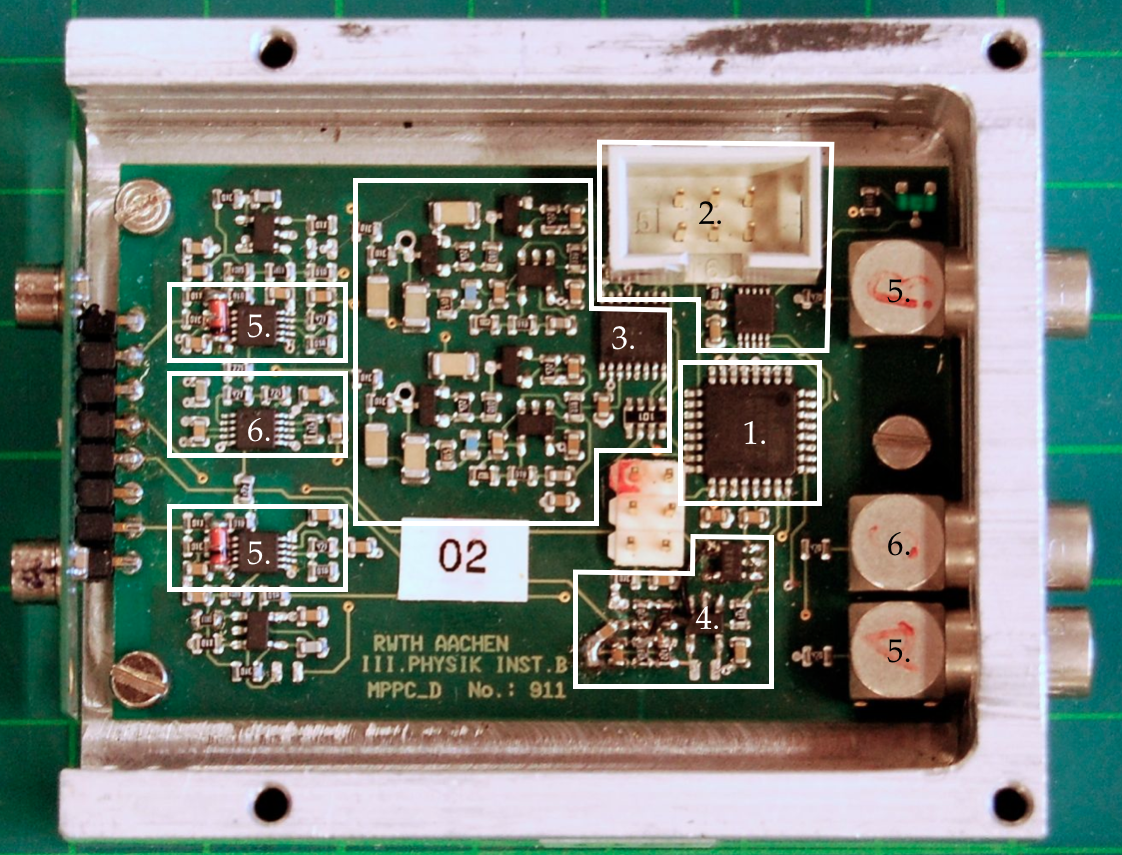
\includegraphics[width=0.5\textwidth]{Figures/weinstock/mppc_d_titled.png}
		\caption{Top down view of the MPPC\_Ds circuitry: 1. ATmega88P with it's 6 pin ICSP header on the bottom left; 
								  2. Boxed 6 pin header for SiPM bus connector;
								  3. Two voltage regulators $0..82\,\text{V}$ (VBIAS) for the SiPMs;
								  4. Pt100 based temperature probe. The Pt100 resistor is located on the front plate between both SiPMs. 
								       It's analog signal is passed to this circuitry;
								  5. Preamplifier and shaper stages and corresponding LEMO outputs; 
								  6. Summing amplifier and LEMO output;
			}
		\label{mppc_top}
	\end{figure}	

\newpage

\subsubsection{Temperature Measurement}

Because of the strong temperature dependency of the SiPMs output pulses a precise temperature measurement is needed to adjust the bias voltage of the SiPMs. The temperature probe of
the MPPC\_D calculates the temperature by measuring the resistance of a Pt100 resistor. The probe's circuit consists of a Wheatstone bridge including the Pt100, an amplifier circuit using
the \emph{MAX4040} OpAmp to compensate the non linearities of the bridge and another MAX4040 OpAmp as a buffer to supply the probe with the
internal Analog Reference (AREF) of $1.1\,\text{V}$ from the microcontroller as shown in Figure \ref{pt100_probe}.

The resistance of the Pt100 changes as follows:
	\begin{equation}
		R_{Pt100}(T) = R_0(1 +\alpha_T T + \beta_T T^2 + \mathcal{O}(T^3)),
		\label{eq_pt100_temperature}
	\end{equation}
where $R_0 = R_{Pt100}(0^{\circ} \text{C})=100\,\Omega$, $\alpha_T = 3.9083 \times 10^{-3}\, \text{K}^{-1}$ and $\beta_T = -5.775 \times 10^{-7}\, \text{K}^{-2}$. To compensate 
the non linear terms in equation \ref{eq_pt100_temperature}, which are lowering the resistance at higher temperatures, current can be fed back to the Pt100 resistor to increase 
the output voltage. The current feedback should be chosen in a manner that the resulting output voltage of the temperature probe changes linear with respect to the temperature.

One also has take into account the non linearities resulting from the Wheatstone bridge. The output voltage $U_{in}$ that is fed into the MAX4040 amplifier is
	\begin{equation}
		U_{in} = U_{ref}(\frac{R_{10}}{R_{10} + R_5} - \frac{R_{11}}{R_{11} + R_6}).
	\end{equation}
As shown in the schematics in Figure \ref{pt100_probe} $R_{10}$ is the Pt100 resistor. One can easily see that the output voltage is not linear dependent on the resistance
of $R_{10}$. To reduce the effect of this non linearity $R_{5}$ is chosen to be larger than $R_{10}$, so that $R_{10} + R_{5} \approx R_{5}$ holds. The resistors $R_6$, $R_9$ and 
$R_{11}$ set the required gain and offset of the amplifier to produce the desired output voltage. 
$R_7$ provides the previously discussed current feedback to the Pt100 resistor depending on the output of the amplifier.

	\begin{figure}[t]
		\centering
			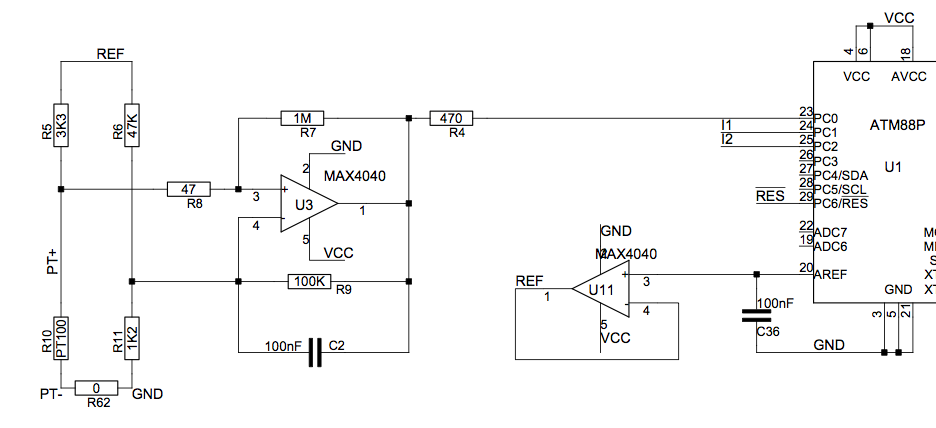
\includegraphics[width=0.7\textwidth]{Figures/weinstock/pt100_probe.png}
		\caption{Schematics of the Pt100 based temperature probe of the MPPC\_D. The resistor $R_{10}$ is the Pt100 resistor.}
		\label{pt100_probe}
	\end{figure}	
 
\subsubsection{Temperature Probe Calibration}

The output voltage of the temperature probe is measured by a $10$ bit ADC on the microcontroller. Internally the temperature then is calculated by the following equation:
\begin{equation}
	T[^{\circ}C] = TGain[^{\circ}C/count] \times ADCcount + TOffset[^{\circ}C]
\end{equation}
The calibration of the temperature probe can be done by simply exposing the probe to a well regulated temperature and reading it's ADC register. The $10$ bit ADC of the microcontroller
can be read out with the command "J". For a fast temperature calibration one also can use a Pt100 simulator. This simulator is a potentiometer that can be set to a certain 
temperature value and outputs the corresponding resistance of a Pt100 resistor at the given temperature value. 

\newpage

\subsubsection{Bias Voltage Supply}

To compensate the temperature effects on the SiPM the bias voltage has to be corrected by a factor of $\frac{\Delta U_{bias}}{\Delta T} = 56\,\frac{mV}{K}$. The MPPC\_D has two 
voltage regulators to apply the correct bias voltage to each SiPM. The schematics of a voltage regulator are shown in Figure \ref{voltage_regulator}. 
	
	\begin{figure}[t]
		\centering
			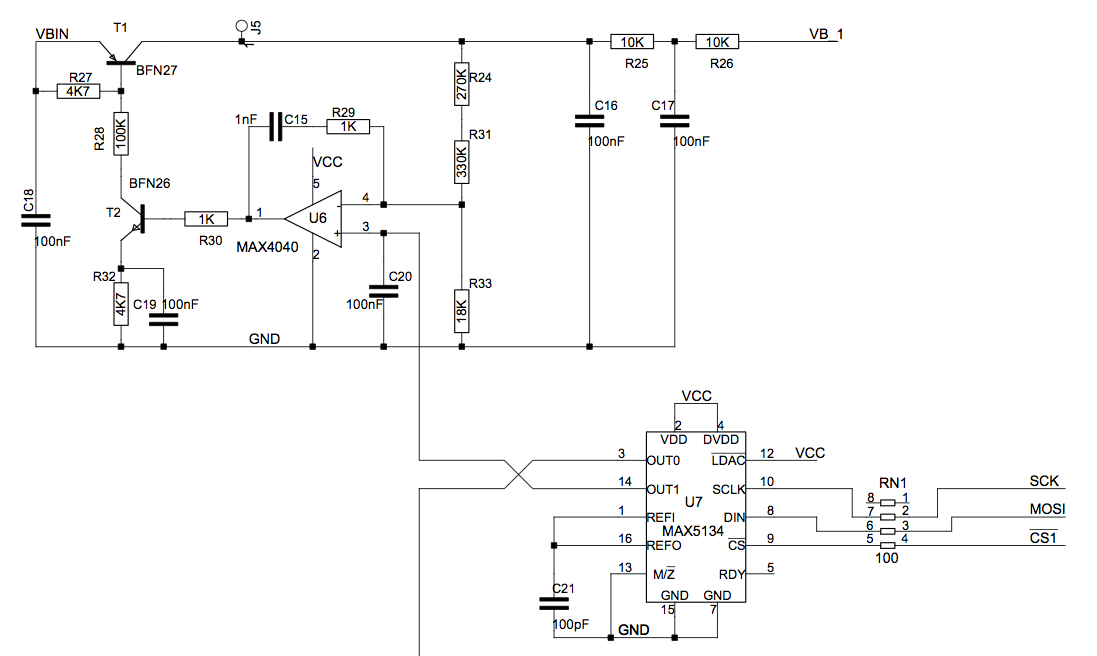
\includegraphics[width=0.7\textwidth]{Figures/weinstock/dac_circuit.png}
		\caption{Schematics of one of the voltage regulators on the MPPC\_D. The regulated bias voltage is output to $VB_1$.}
		\label{voltage_regulator}
	\end{figure}	

The voltage regulators use a Pulse Width Modulation (PWM) signal to adjust the bias voltages. PWM is used to reduce power consumption.
The core parts of the voltage regulator are two high voltage transistors $T_1$ and $T_2$ and an integrating amplifier circuit built around another MAX4040. The integrator increases
it's output voltage as long as the voltage drop at the divider $R_{24}$, $R_{31}$ and $R_{33}$ is below the voltage input of the 16 bit MAX5134 DAC.
The voltage on the voltage divider is increased by the output of $T_1$ which again is influenced by the amplifier's output. The result of this feedback is a rectangular output
pulse at $T_1$. The duty cycle of this pulse is determined by ratio of the voltage given by the DAC and the voltage drop of the divider:
	\begin{eqnarray}
		D &=& \frac{T}{P} = \frac{U_{dac}}{U_{div}} \\
		U_{div} &=& \frac{R_{33}}{R_{24} + R_{31} + R_{33}} U_{bin} = 2.46\,\text{V},
	\end{eqnarray}
where $T$ is the time the signal is active, $P$ the total period of the signal ($P$ is determined by the values of $C_{22}$ and $R_{29}$) and $U_{bin}=82V$ the voltage provided by the 
APDPIs VBIAS line. The output voltage of the DAC ranges from $U_{dac}=0\, \text{V} .. 2.44\, \text{V}$ (internal reference). The PWM output is then filtered by the two high passes 
$R_{25}$, $C_{16}$ and $R_{26}$, $C_{17}$ ($f_{crit} = \frac{1}{2 \pi RC}$) and transferred to the SiPM. The applied bias voltage is then defined by the duty cycle of the former 
PWM signal:
	\begin{equation}
		U_{bias} = U_{bin} D = U_{bin} \frac{U_{dac}}{U_{div}}.
	\end{equation}

\subsubsection{Bias Voltage Regulator Calibration}
The output voltage of the DAC is set by accessing the output registers. The output registers can be set to any value between \verb|0x0000| .. \verb|0xFFFF|, setting the output to 
$0\, \text{V}..2.44\, \text{V}$ respectively. To get the precise conversion from DAC counts to output bias voltage one must perform a calibration of the DACs. Internally 
the bias voltage set by the following calculation:
	\begin{eqnarray}
		DACcounts &=& DACOffset + U_{adj}[5\,mV]/DACGain \\
		U_{adj} &=& \frac{\Delta U_{bias}}{\Delta T}(T - 25\,^{\circ} \text{C}) + U_{adj}(25\,^{\circ} \text{C}),
	\end{eqnarray} 
where $U_{adj}$ is the temperature adjusted bias voltage and $\frac{\Delta U_{bias}}{\Delta T} = 56\,\frac{\text{mV}}{\text{K}}$. 

To calibrate the DAC the module has to be set to DAC calibration mode by issuing the command "Q". In calibration mode $DACOffset$ and $\frac{\Delta U}{\Delta T}$ 
are set to $0$ and $DACGain$ to $1$ thus disabling the temperature correction. Also one can now access the DACs registers directly by setting the bias voltage 
at $25^{\circ} \text{C}$ with the command "Dhhhh" or "Ehhhh" to the hex value $5\times\verb|0xhhhh|$. By setting the DAC output registers to a given value and then measuring the 
output adjusted bias voltage one can easily perform a calibration.

\subsubsection{Amplifier Circuits}

The MPPC\_D uses Current Feedback Amplifiers (CFA) instead of Voltage Feedback Amplifiers (VFA) because of the superior gain-bandwidth product of these amplifiers. A high 
gain-bandwidth product is needed because the Geiger discharges on the SiPM create high speed rising edges. The steep rising edges provide the fastest information of an incoming photon. 
By not distorting these high speed components the trigger information becomes avaliable faster.

The amplifier chip used on the MPPC\_D is the \emph{MAX4228} which has a bandwidth of $1\,\text{GHz}$ at unity gain. The whole amplifier circuit is shown in Figure \ref{fig:amp_cir}. 
The first amplification stage is a transimpedance amplifier. This preamplifier converts a current signal into a voltage signal:
\begin{equation}
	U_{preamp} = R_{20} I_{sig},
\end{equation}
where $R_{20} = 1\,\text{k}\Omega$. The second stage is a non-inverting amplifier, but only half the preamplifier's signal reach this step for the other half is fed to the summing amplifier:
\begin{equation}
	U_{out} = \frac{1}{2} (1 + \frac{R_{23}}{R_{22}}) \, U_{preamp} = 2.85 \, U_{preamp}.
\end{equation}

	\begin{figure}[t]
		\centering
			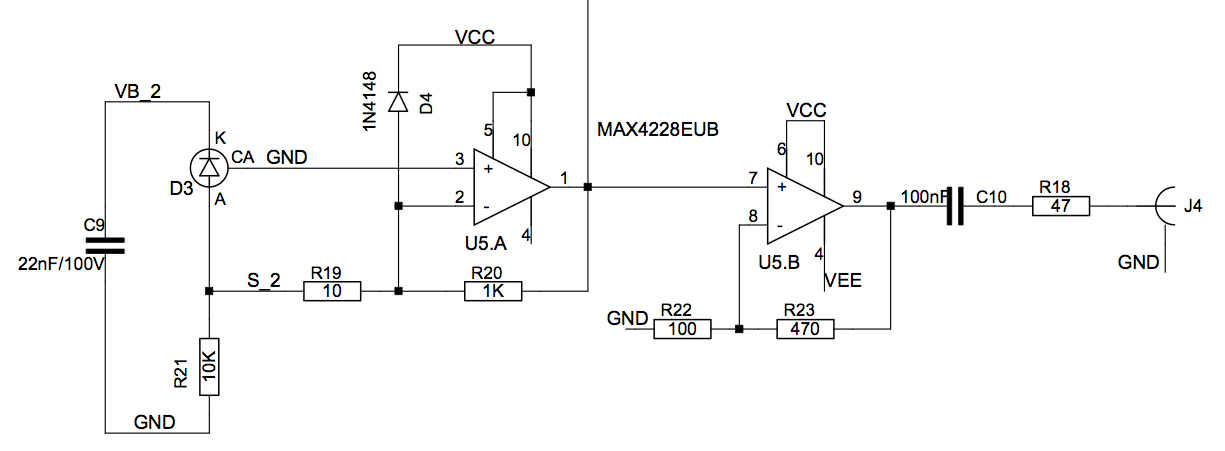
\includegraphics[width=0.7\textwidth]{Figures/weinstock/amplifier_circuit.png}
		\caption{Schematics of one of the amplifier circuits. The first stage is the tansimpedance preamplifier, the second is a non-inverting amplifier. The capacitor is used to decouple the AC from the DC components since we are only interested in the AC components of the pulse.}
		\label{fig:amp_cir}
	\end{figure}	
The summing amplifier shown in Figure \ref{fig:sum_amp} adds the signals of both preamplifiers and amplifies them again by a factor of $\approx4.5$. So in total the sum signal is about $80\%$ smaller than the single channel signal.

	\begin{figure}[t]
		\centering
			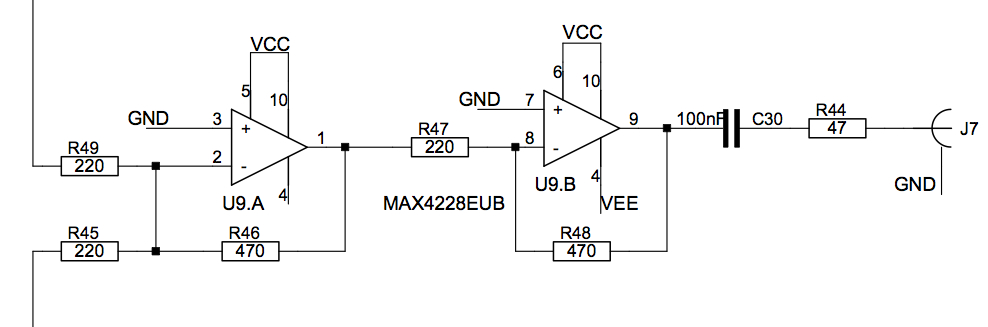
\includegraphics[width=0.7\textwidth]{Figures/weinstock/sum_amp.png}
		\caption{Summing amplifier of the MPPC\_D. The inputs of the first amplifying stage come directly from preamplifiers.}
		\label{fig:sum_amp}
	\end{figure}	

	
One of the drawbacks of CFAs is that they have a high offset current which results in a offset voltage of about $U_{off,CFA}\approx \pm 1\,\text{V}$. Because we are only interested in the AC components of the signal we use $C_{10}$ as a decoupling capacitor. The resistor $R_{18}$ adjusts the lines impedance to the resistance of a LEMO cable to reduce current reflections.

Figure \ref{fig:sipm_pulse_old} shows a 1 P.E. output from the amplifier stages. The pulse height is about $U_{1p.e.} = 25\,\text{mV}$ and the total pulse duration $T_{pulse} = 80\,\text{ns}$. Figure \ref{fig:rise_time_old} shows a rise time distribution for $10,000$ SiPM pulses. As one can see the rise time of an average SiPM pulse is at about $t_{rise} = 5\,\text{ns}$.

	\begin{figure}[t]
		\centering
			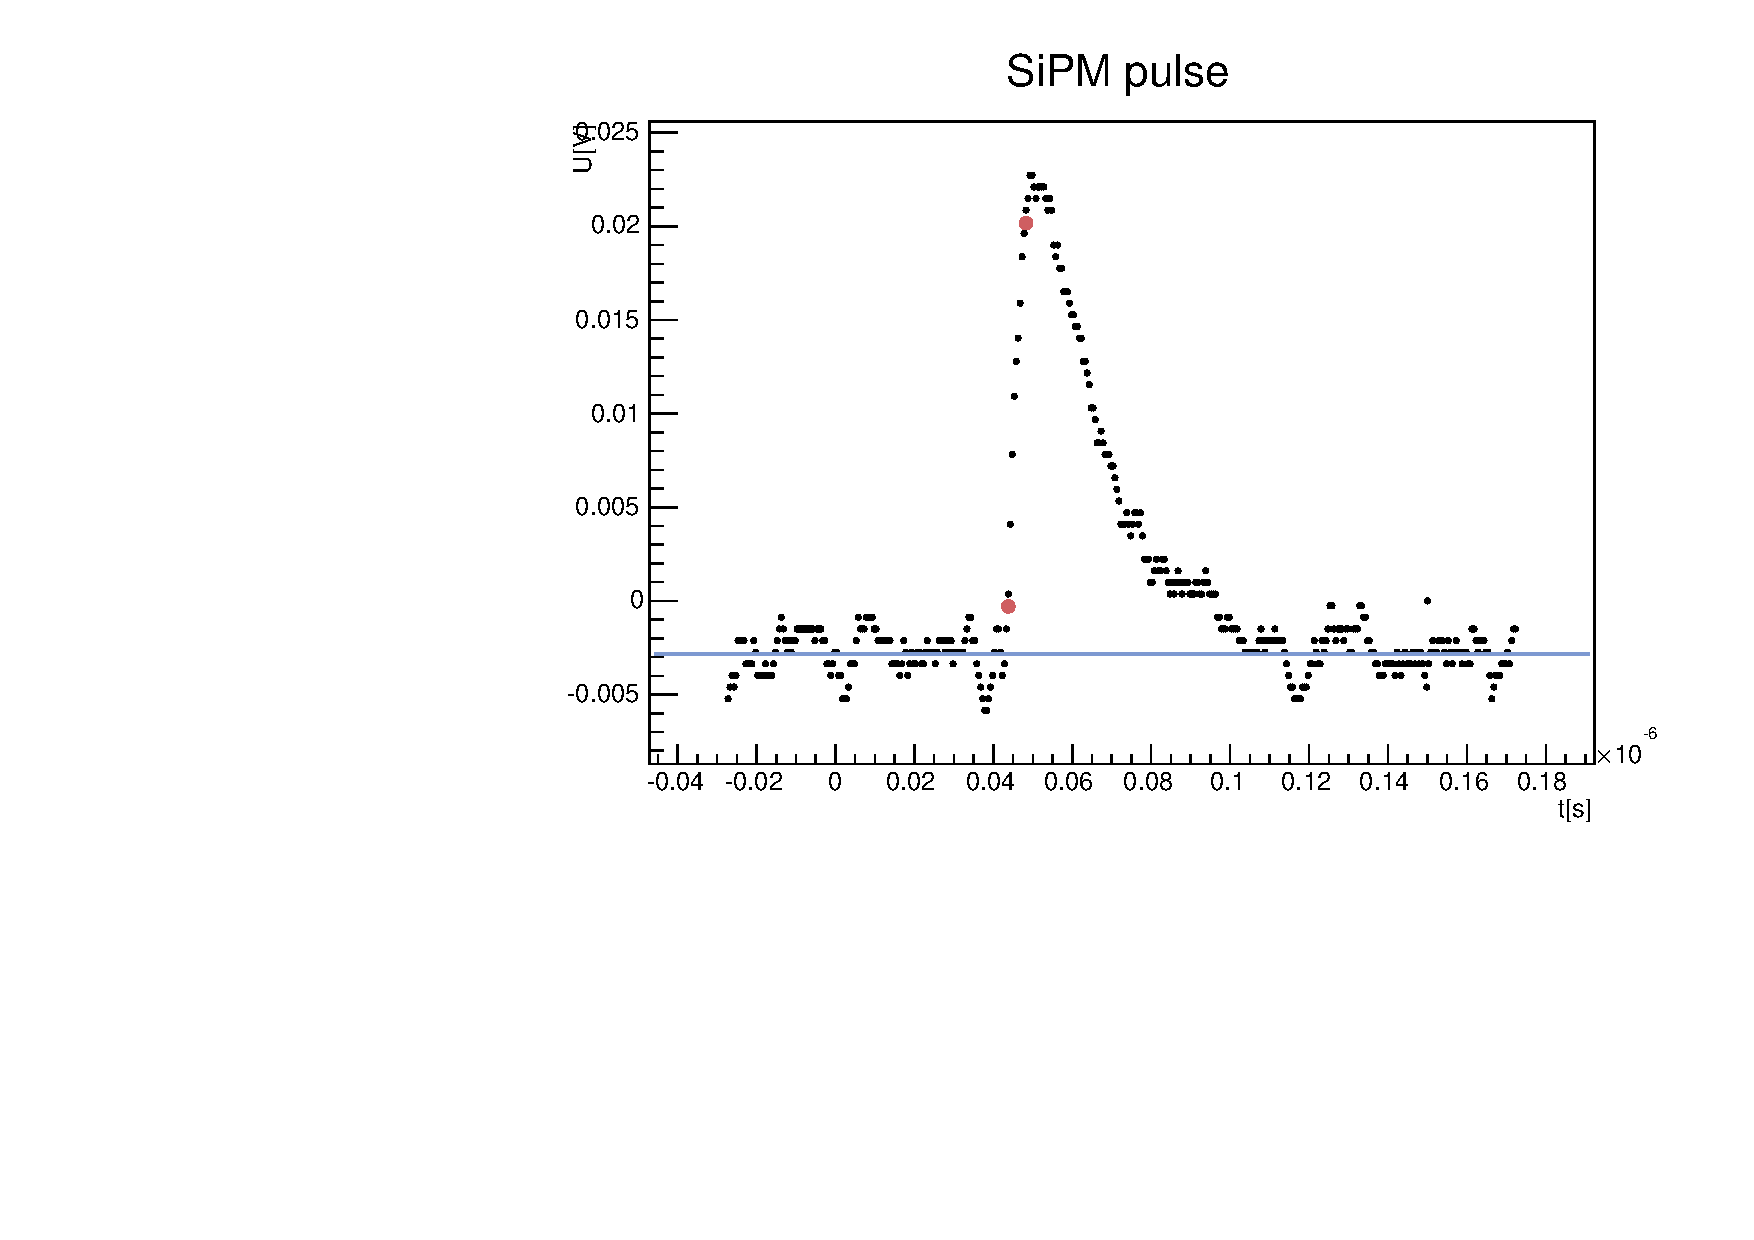
\includegraphics[width=0.7\textwidth]{Figures/weinstock/old_amp_1pe.pdf}
		\caption{1 P.E. output pulse of the SiPM after amplification by the MPPC\_D. The blue line is the reconstructed baseline, the red dots are the $10\%$ and $90 \%$ marks of the pulse height. They are used to calculate the rise time.}
		\label{fig:sipm_pulse_old}
	\end{figure}
	
	\begin{figure}[t]
		\centering
			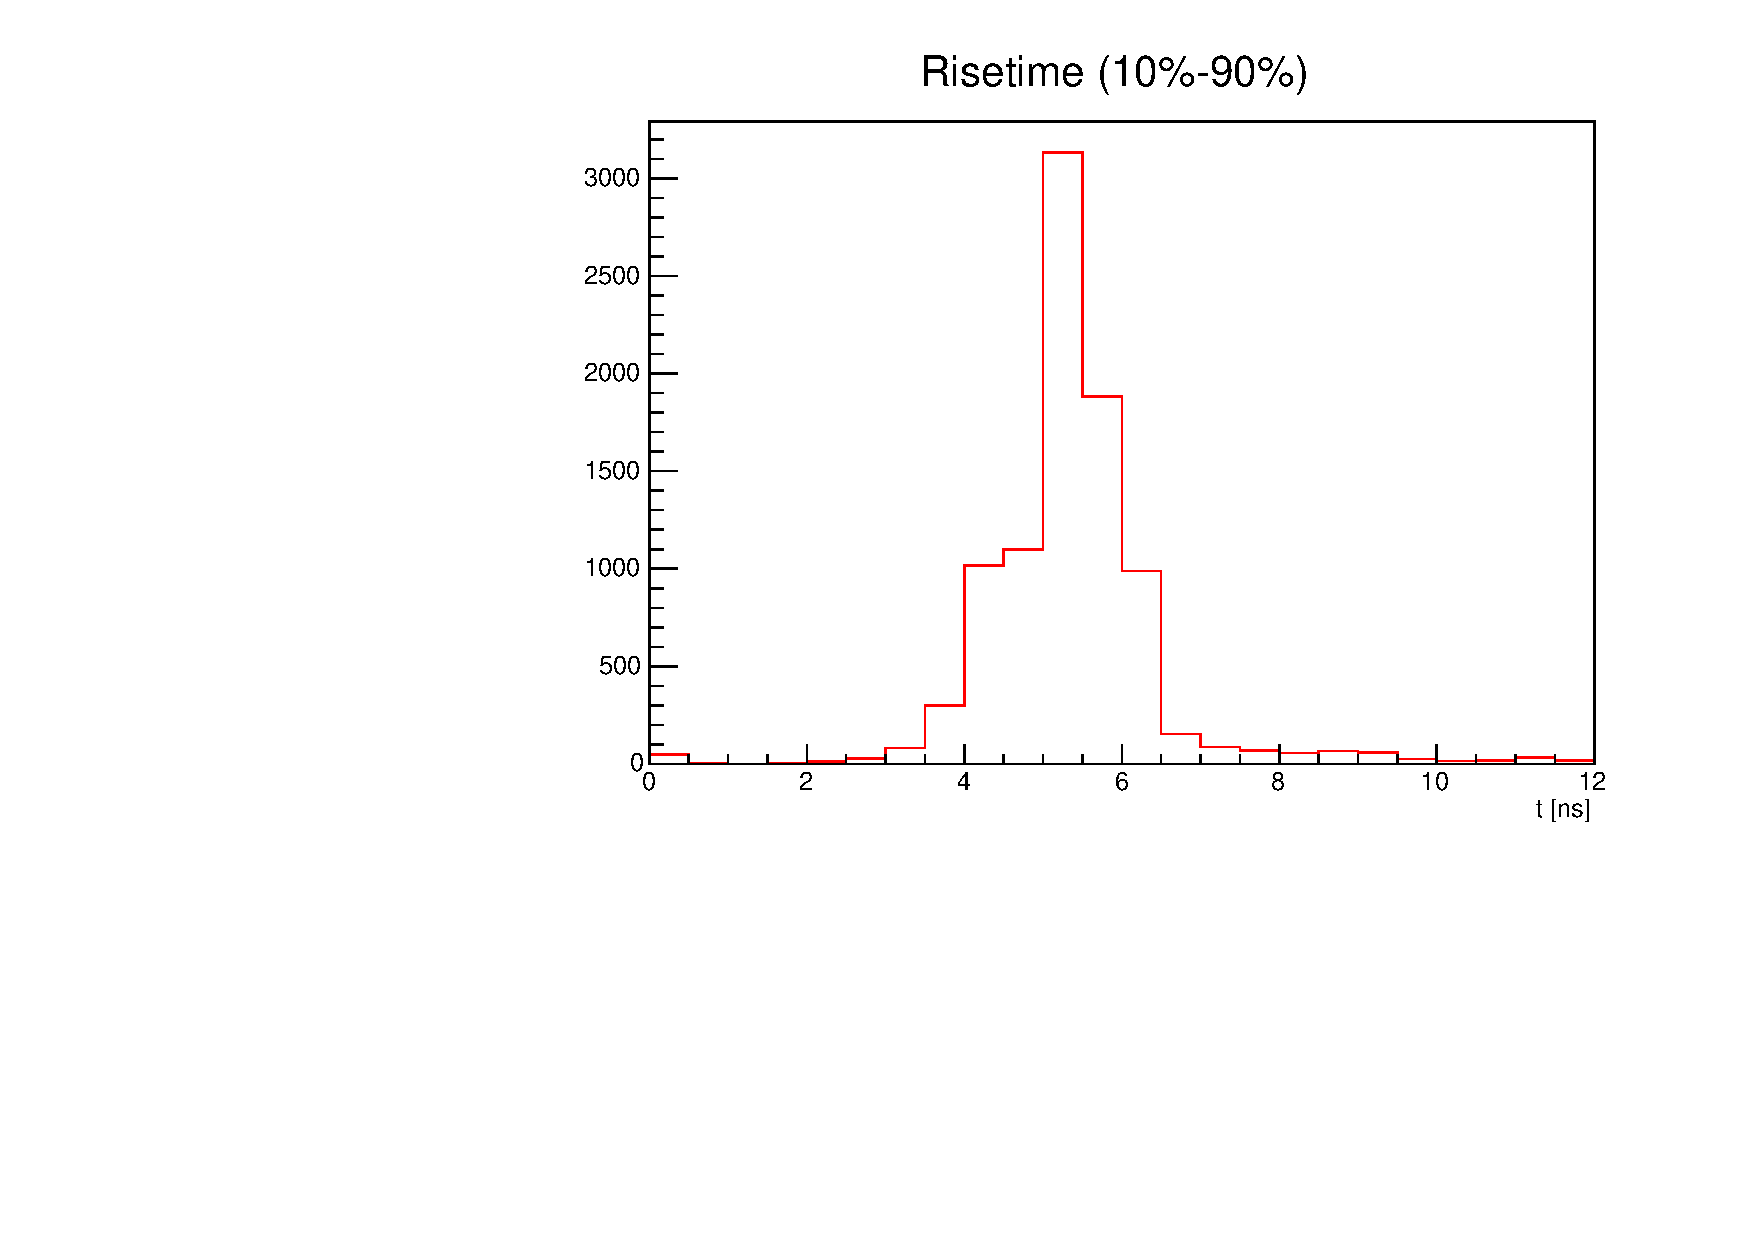
\includegraphics[width=0.7\textwidth]{Figures/weinstock/old_amp_rise_time.pdf}
		\caption{Distribution of rise times of $10,000$ SiPM pulses amplified by the MPPC\_D amplifier stages.}
		\label{fig:rise_time_old}
	\end{figure}	

\subsubsection{Overview Of Technical Characteristics}

\subsection{Appendix: Circuit Diagrams}

\end{document}

\newpage
\section{Studies on Silicon Photomultiplier}
\label{sipmChapter}
\subsection{Studies of noise peak movement under temperature variation}
Since we are using SiPMs with a sensitive area of $3\times3\,\mathrm{mm}$ we discovered a clipping in our frontend electronics due to higher signals. Therefore we had to set down the amplification factor. This implicates that individual p.e. peaks were not observable anymore. Therefore the possiblity to regulated the bias voltage on temperature variation by measuring the asymmetry of the edges of the first p.e. to keep it on a constant value could not be realized in that way. But a implementation of this algorithm on the entire noise peak could be possible which leads to these studies.

\subsubsection{Testsetup}
To measure the movement of the noise peak under temperature variation a prototyp frontend without scintillator was put in a cooling box which could be regulated with the temperature device located between the two SiPMs. The bias voltage supplied to the SiPM was fixed to a constant value. The fingerspectra based on the peakheights was collected from pulses taken with an FADC. Thereby the peakheights were defined as the potential difference between the pulse maximum and the average baseline. The FADC was triggers itselves on pulses over $0.5\,\mathrm{p.e.}$. To avoid influence from pedestals only one SiPM-Channel was regarded. To analyse the peak a fit of an exponentially modified gaussian distribution was used due to best match to the shape.

\subsubsection{Results}
As one can see in figure \ref{NoiseMove} the mean of the noise peak shifts linear to smaller peakheights with increasing temperature based on the decreasing overvoltage. Also the peak width gets smaller because the gain drops with the decreasing overvoltage. Based on this it is possible to adjust the bias voltage by the movement of the noise peak.
\begin{figure}[h]
	\centering
	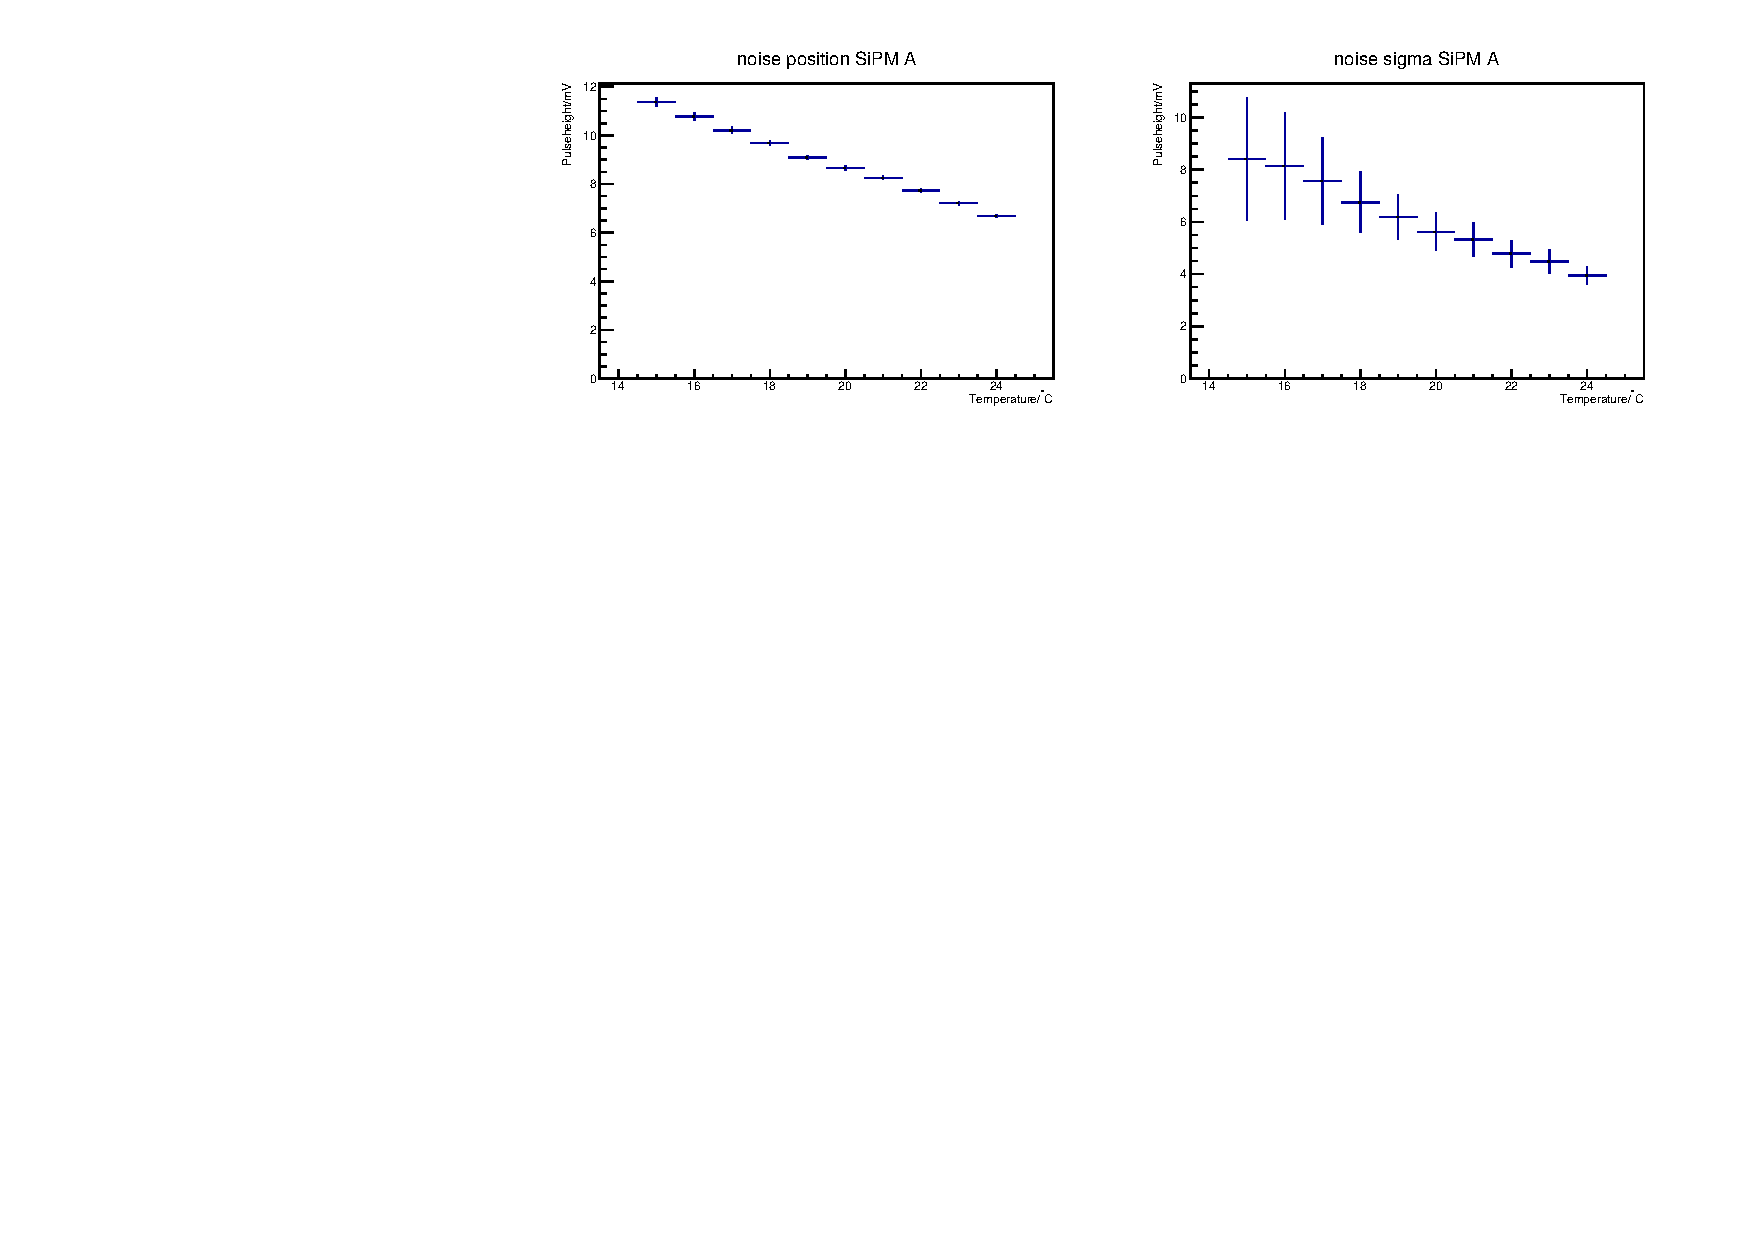
\includegraphics[width = .99\textwidth]{Figures/radermacher/result_ExpGauOnlySipmATriggerNEW.pdf}
	\caption{measurement of noise peak movement}
	\label{NoiseMove}
\end{figure}

\subsection{Performance of gain and noiserates by temperature variation}
Since signals of Silicon Photomultipliers are very sensible to temperature changes, there is an advantage of studying the gain and noiserate depending on the device temperature. Actually the signal depending on gain should stand the same while running data taking phases. Therefore the bias voltage supplied to the SiPM have to be adjusted under temperature changes. For this reason producers for SiPMs like Hamamatsu whose products we use for our prototyps give a temperature regression coefficient which have to be validated. For our prototyp we also check alternative methods to keep the gain constant due to the fact that measurements of temperature are not very precisely nor it is not checkable if it is the real temperature of the semiconductor.

\subsubsection{Testsetup}
To measure the performance under temperature variation a setup was built up including a cooling box, which was used in the testphase of the silicion strip modules here in aachen.
A version of our frontend board with an higher amplification factor was make use of which could be controled with an external power supply, given the bias voltage to the SiPM. For the measurement of gain and noiserate the outcoming signal was splitted over a Fan-Out and routed to a FADC and a scaler.
The FADC triggers itselves on every flank over $0.5\,\mathrm{p.e.}$. The given pulses then were analysed online and the peakheights were filled into an histogram producing a so called fingerspectrum.
Afterwards the first three p.e.-peaks were fitted by gaussian function and a combination of them were taking as the gain factor which is defined as the distance between two p.e.-peaks.
The line to the scaler were taking to measure the noiserate by connecting a LTD in front of the scaler which discriminates signals over $0.5\,\mathrm{p.e}$.
In total there were three measurement methods to check the changement of the parameter. This three listed in following were done with two several series of SiPMs, S10362-33-050C and S12572-050C.
A sketch of the setup is shown in figure \ref{NoRa_DAQ}. 
\begin{figure}[h]
	\centering
	\includegraphics[width = 0.5\textwidth]{Figures/radermacher/NoRa_DAQ_en.pdf}
	\caption{DAQ-Chain for measurements with SiPMs under temperature variation}
	\label{NoRa_DAQ}
\end{figure}
\begin{description}
	\item[Measurement of noiserates by constant gain]: For this method the gain was checked every temperature step and the bias voltage were corrected until the gain was the default value. Afterwards the noiserate were measured over the LTD with a threshold on $0.5\,\mathrm{p.e.}$. With this measurement method it was also possible to check the temperature coefficient.
	\item[Measurement of noiserates and gain by constant bias voltage]: In this measurement simply the bias voltage was fixed to a certain value and every step of temperature the gain and the noiserate was measured.
	\item[Measurement of noiserates and gain by constant temperature]: Here the temperature was fixed and the bias voltage were raised in little steps. 
\end{description}

\subsubsection{spectra analysis}
The spectra one get from this measurements are shown in figure \ref{fingerspecs}. As one can see, there are some differences between the two tested SiPMs. The spectrum of the older version S10362-33-050C shows nearly overlapping p.e. peaks which could not seperated very clearly. Otherwise the noise spectrum only has up to $3\,\mathrm{p.e.}$. The S12572-050C series in contrast shows more than $5\,\mathrm{p.e.}$. On the other hand the p.e.-peaks are clearly seperated which leads to a better gain determination.
\begin{figure}[h]
	\centering
	\begin{minipage}[b]{0.49\textwidth}
		\includegraphics[width = .99\textwidth]{Figures/radermacher/S10362-33-050C.pdf}
	\end{minipage}
	\begin{minipage}[b]{0.49\textwidth}
		\includegraphics[width = .99\textwidth]{Figures/radermacher/S12572-050C.pdf}
	\end{minipage}
	\caption{fingerspectra for the testes SiPMs}
	\label{fingerspecs}
\end{figure}
\subsubsection{constant gain}
For the measurements with constant gain the value for the gain was assigned by using the given default voltage for $25\,\mathrm{^{\circ}C}$ while the cooling box was regulated to $25\,\mathrm{^{\circ}C}$. Afterwards the temperature was reduced in steps of 1 degree in a range between $25$ and $15\,\mathrm{^{\circ}C}$. Every step the gain was measure and controlled if it is the same as the default gain. Till this was reached the supplied voltage was regulated that one get the desired circumstances. Afterwards the noiserate was measured as shown in figure \ref{constGain_rate}.
As expected the noiserate increases with temperature due to thermally-generated carriers. Also one can see that the newer Hamamatsu product has significant higher noiserates.
\begin{figure}[h]
	\centering
	\includegraphics[width = 0.75 \textwidth]{Figures/radermacher/constGain_Rate.pdf}
	\caption{noiserate under temperature variation with constant gain}
	\label{constGain_rate}
\end{figure}
As a second result from this measurements it was possible to check the temperature regression coefficient. These values are given by Hamamatsu for every SiPM-Serie. For the S10362-33-050C the coefficient is predicted to $56\,\mathrm{mV/K}$, for the S12572-050C it is $60\,\mathrm{mV/K}$. Our measurements are in good agreement to this with $(56.6 \pm 0.5)\,\mathrm{mV/K}$ for S10362-33-050C and $(59.7 \pm 0.7)\,\mathrm{mV/K}$ for S12572-050C SiPMs. The results are shown in figure \ref{tempCoeff}. 
\begin{figure}[h]
	\centering
	\begin{minipage}[b]{0.49\textwidth}
		\includegraphics[width = 0.98\textwidth]{Figures/radermacher/TempReg_S10362.pdf}
	\end{minipage}	
	\begin{minipage}[b]{0.49\textwidth}
		\includegraphics[width = 0.98\textwidth]{Figures/radermacher/TempReg_S12572.pdf}
	\end{minipage}
	\caption{Determination of the temperature progression coefficient}
	\label{tempCoeff}
\end{figure}

\subsubsection{constant bias voltage}
To measure the noiserate by keeping the bias voltage constant the voltage was set to the default voltage at $25\,\mathrm{^{\circ}C}$ and the temperature was regulated between $25$ and $15\,\mathrm{^{\circ}C}$ in steps of 1 degree. As shown in figure \ref{constVolt_rate} there is a linear increase with temperature. These increase is much higher for the newer Hamamatsu product S12572 with $39.4\,\mathrm{\%}$ as for the S10362-33-050C with $26.5\,\mathrm{\%}$ over a range of $10\,\mathrm{^{\circ}C}$. 
The gain otherwise shows a linear decrease with temperature due to the higher overvoltage on lower temperature as one can see in figure \ref{constVolt_gain}. The plateau by $15 - 17\,\mathrm{^{\circ}C}$ arised from smeared fingerspectra.  
\begin{figure}[h]
	\centering
	\includegraphics[width = 0.75 \textwidth]{Figures/radermacher/ConstVolt_Rate_linear.pdf}
	\caption{noiserate under temperature variation with constant bias voltage}
	\label{constVolt_rate}
\end{figure}
\begin{figure}[h]
	\centering
	\includegraphics[width = 0.75 \textwidth]{Figures/radermacher/constVolt_Gain.pdf}
	\caption{Gain under temperature variation with constant bias voltage}
	\label{constVolt_gain}
\end{figure}
\subsubsection{constant temperature}
For measuring the noiserates with constant temperature this was set to $25\,\mathrm{^{\circ}C}$ and the bias voltage was raised in $50\,\mathrm{mV}$-steps. With more bias voltage the noiserate increase linear. Under these circumstances it is much higher for the S10362-33-050C with $62.8\,\mathrm{\%}$ instead of $16.0\,\mathrm{\%}$ for the S12572-050C over the range of $450\,\mathrm{mV}$ shown in figure \ref{constTemp_rate}. The trend of the gain as one can see in figure \ref{constTemp_gain} is not analytic but looks quite equal for both SiPMs.
\begin{figure}[h]
	\centering
	\includegraphics[width = 0.75 \textwidth]{Figures/radermacher/ConstTemp_Rate_linear.pdf}
	\caption{noiserate under variation of bias voltage with constant temperature}
	\label{constTemp_rate}
\end{figure}
\begin{figure}[h]
	\centering
	\includegraphics[width = 0.75 \textwidth]{Figures/radermacher/constTemp_Gain.pdf}
	\caption{Gain under variation of bias voltage with constant temperature}
	\label{constTemp_gain}
\end{figure}
\subsubsection{conclusion}
The measurements shown the expected behaviour on temperature variations. The temperature regression coefficient given by Hamamatsu has been certified and some quality criteria were studied. With help of this we choose to use the S10362-33-050C for our prototyp detectors until a newer SiPM-serie is presented because there are not enough improvements by using the S12572-050C due to clipping of the amplifier mentioned in chapter HIER KAPITEL UEBER NOISEPEAK EINFUEGEN. Therefore the higher gain is not needed and will maybe produce more signals in clipping. Unless a controlling of the bias voltage due to temperature change by counting in the asymmetry of the p.e. is done a better peaksresolution is not needed.

\subsection{Determination of Bias Voltage for new MTT-Prototyps}
\label{sipmVoltDetermination}
In order to get same signals independtly from our prototyps, a determination for the bias voltage is done by commiting the same gain for every SiPM. This should assure that QDC- and Peakheightspectra look the same regardless of the used prototyp module. After verify the temperature regression coefficient the signal spectra is only depending of the gain given by the supplied bias voltage.

\subsubsection{Experimental Setup}
To determinate the needed bias voltage to a specified gain a simple teststand is built up with an LeCroy WaveJet354A oscilloscope and a cooling box. With the oscilloscope a signal trace of $500\,\mathrm{\mu s}$ is taken from which a fingerspectrum is formed. Therefore the trace is derived after flattening and the peaks in the derived spectrum are searched. Afterwards the actual pulsepeaks are determined from the peaks out of the derived spectrum by searching of the next maximum after the slope you get from peaks of the derived spectrum. 
In addition the minimum in front of the slope is determined as baseline belonging to the peak. Out of that the fingerspectrum is built by the pulseheight defined as the difference between pulsemaximum and the belonging baseline.
From the fingerspectrum the gain is determined by identification of the first two p.e. and calculation of the gain defined as the difference between them. For the bias voltage a algorithm checks if the measured gain is in agreement with the specied one elsewise it modifies the voltage till it fits.

\subsubsection{Distribution Analysis to Parameter Determination}
In progress...    


\section{Muon ghosts}
\subsection{The DT System}
\label{DTSystem}
The drifttube (DT) system of the muon detector at CMS consists of several organization structures.\\
The smallest structure, the drift tubes are organized within a superlayer (SL). A superlayer consists of four layers of DTs. Every sector per wheel in CMS has four muon stations, counted 1 to 4 beginning with the inner most station.\\
A muon station is the composition of two SLs oriented in $\phi$ direction (stations 1-4) and one SL in $\theta$ direction (stations 1-3). The readout hardware of one station is assembled in a minicrate (MC).\\
The trigger chain of the DT system starts within a SL. Nine of the DTs are combined to a bunch and track identifier (BTI) Trigger. BTI Triggers have an overlap region to avoid inefficiencies and to obtain redundancy. If three of four DTs see a signal for a certain bunch crossing, a low quality trigger (LTRG) is generated. If four DTs in line see a signal, a high quality trigger (HTRG) is generated. For now, only HTRG are processed in the next trigger step.\\
The track correlator (TRACO) combines the HTRG of the two BTIs of the SL in phi direction within one station. TRACO triggers can be generated for muons with an angle of $45^{\circ}$ \cite{bunchedBeamTest} or less.\\
These TRACO triggers are transmitted via 40 line flat cables to the trigger server (TS). The TS is located on the MC of station 4.\\
The TS consists of a phi and a theta part. The TS phi correlates the TRACO tracks in phi direction. The TS theta correlates the tracks in $\theta$.\\
This data is transmitted via low voltage differential signaling (LVDS) to the sector collector (SC) that is located in the service cavern (USC).\\
From there the signal is processed to the global muon trigger (GMT) and the global trigger (GT).
For the setup of the muon trigger system, see also \cite{cmsMuonProject}.
\subsection{Reconstruced Ghosts}
\subsubsection{Ghost definition}
Ghosts are faked muons that are detected by the muon system although there is no physical muon present.
Muon ghosts can occur in all stages of the detection and reconstruction system of CMS beginning with the low level triggers up to the final reconstructed data (Fig. \ref{fig:ghosts}).
A ghost can also be a detected muon that has the wrong time stamp and thus is assigned to the wrong bunch crossing.

\subsubsection{Reco ghosts}
Following the definition of ghosts, a RECO ghost is a reconstructed muon that has no matching generated (GEN) muon.\\
For this matching, for every RECO muon the nearest GEN muons in terms of $\Delta R$ is determined. Additionally, the vertex position of the GEN and RECO muon must not be displaced by $>$ 0.1 cm in every of the three coordinates to assure that the RECO muon is not from a pileup event.\\
The following investigations are performed with global muons only, to have muon system and tracker information available for every muon. Furthermore, the eta direction of the investigated muons is cut to be abs(eta) $<$ 0.8 to check for muons in the barrel region only. The sample is a ZZ$\to$4l with 2012 conditions.\\
$\Delta R$ is plotted for all GEN muons with their matched RECO muon. If two RECO muons match the same GEN muon, $\Delta R$ is plotted for both RECO muons.\\
The $\Delta R$ distribution is shown in Fig. \ref{DeltaRDistribution}. Most of the matched muons have a very small $\Delta R$. Only a few muons have a $\Delta R$ above 0.1 with a slight maximuim at 1.5. It is obvious that the most muon combinations with $\Delta R > 0.1$ come from muons in ghost events. Therefore, a separation between ghosts and real muons using $\Delta R$ seems to be feasible and is discussed.\\
\begin{figure}[b]
\centering
\begin{minipage}[t]{0.95\textwidth}
\includegraphics[width=\textwidth]{Figures/scheuch/Trennung.png}
\caption{$\Delta R$ between all RECO muons and the matched GEN muon in all events and in events that are marked as ghost events}
\label{DeltaRDistribution}
\end{minipage}
\end{figure}
If one GEN muon has two or more associated RECO muons all but one of these RECO muons are considered to be ghosts. An event with at least one ghost is named ghost event.\\
For the separation whether a RECO muon is a ghost or real, a $\Delta R$ cut is introduced. If the $\Delta R$ between RECO muon and associated GEN muon is smaller than 0.1, the muon is considered to be a correctly reconstructed muon. If the $\Delta R$ is greater than 0.1, it is considered to be a ghost.

\subsubsection{Matching efficiency and quality of separation}
To determine whether the matching algorithm is correct and efficient, some control variables have been observed.\\
The distance of vertex position in the z direction (meaning along the beam axis) of the RECO muon and the associated GEN muon was plotted (see figure \ref{DeltaZMatching}). The distance is within the resolution of the tracker system. Nevertheless, all muons with a distance of more than 0.1 cm are rejected, since for large distances in the z vertex a mismatching can not be imposed.\\
\begin{figure}[b]
\centering
\begin{minipage}[t]{0.95\textwidth}
\includegraphics[width=\textwidth]{Figures/scheuch/DeltaZ.png}
\caption{Distance of the z position of the vertex RECO muon and the matched GEN muon}
\label{DeltaZMatching}
\end{minipage}
\end{figure}
To show that the determination between ghost and real muon is reliable, the $p_{T}$ ratio between GEN muon and RECO muon is plotted for identified ghosts (see figure \ref{PtRatioGhost}) and real muons within a ghost event (see figure \ref{PtRatioReal}).
\begin{figure}[b]
\centering
\begin{minipage}[t]{0.475\textwidth}
\includegraphics[width=\textwidth]{Figures/scheuch/ptRatioRealMu.png}
\caption{$\mathrm{p_{T}}$ ratio of the GEN and RECO mu for identified real RECO muons}
\label{PtRatioReal}
\end{minipage}
\hspace{0.5cm}
\begin{minipage}[t]{0.475\textwidth}
\includegraphics[width=\textwidth]{Figures/scheuch/ptRatioGhosts.png}
\caption{$\mathrm{p_{T}}$ ratio of the GEN and RECO mu for identified RECO ghosts}
\label{PtRatioGhost}
\end{minipage}
\end{figure}
The $p_{T}$ ratio peaks at 1 for real muons. This indicates that the RECO muon is in fact the correct reconstruction of the generated particle. On the other hand, the $p_{T}$ ratio of the ghost muons shows a non peaking shape. Therefore, it can be assumed that the $p_{T}$ of the ghosts is not related to the matched GEN particle. The $p_{T}$ of the ghost is smaller than the $p_{T}$ of the generating particle in the majority of ghost events.\\
Furthermore, under the assumption that there is one ghost per real muon only in the majority of the events one expects that the number of ghosts and real muons is equal for a certain GEN muon. Comparing the number of ghosts (12175) and the number of real muons (12013) shows that the seperation between the real and the ghost muon is working well.

\subsubsection{Ghost busting with HO information}
To determine whether hadron outer (HO) information can be used to bust ghosts on L1 Level, the whole calorimeter (including HCAL and ECAL) information is used for 2012 simulations, since HO did not work properly during this phase. In a first step, the likelihood ratio of the calorimeter system (ECAL, HCAL, HO) defined as
\begin{equation}
L=\frac{L_{\mathrm{muon}}}{L_{\mathrm{muon}} + L_\mathrm{not\ muon}}
\end{equation}
is plotted.
\begin{figure}[b]
\centering
\begin{minipage}[t]{0.95\textwidth}
\includegraphics[width=\textwidth]{Figures/scheuch/LikelihoodNonGhost.png}
\caption{Likelihood ratio for an MIP like entry in the calorimeter system for real muons}
\label{LikelihoodReal}
\end{minipage}
\end{figure}
\begin{figure}
\begin{minipage}[t]{0.95\textwidth}
\includegraphics[width=\textwidth]{Figures/scheuch/LikelihoodGhost.png}
\caption{Likelihood ratio for an MIP like entry in the calorimeter system for ghosts}
\label{LikelihoodGhost}
\end{minipage}
\end{figure}
For identified muons the likelihood ratio peaks at 1. This is consistent with the fact that real muons should deposit energy within the calorimeter system.\\
The likelihood ratio for ghosts peaks at 0, has a miminum at 0.4, and rises again up to 1 without reaching a maximum at 1. The ghosts should not deposit energy in the calorimeter system. For some of the ghosts this seems to be the case. For the other ghosts the likelihood might be tending to 1 because energy is deopsited in the calorimeter system by other particles or due to some noise. This can also explain why the likelihood ratio drops at the 1st bin for ghosts.\\
In a next step, the energy information in the HO system for an HO tower has to be investigated to obtain whether HO can serve as muon veto and trigger. This has to be redone also for HL-LHC conditions. Here, one has to check whether the granularity of HO is sufficient to deal with the additional pile up and boosted events.
\subsection{BTI Ghosts}
\subsubsection{Ghost definition}
If only one muon passes a muon station and two BTI HQTR are created in this station it is called BTI ghost. (For the description of the BTI system see chapter \ref{DTSystem}.)
\subsubsection{Investigation of the BTI Trigger}
To see whether the BTI triggers experience ghost phenomena, a muon gun study was performed. Events without pileup were created. Every event contains one muon that is passing directly through one of the 12 sectors. This muon hits all four muon chambers. A second muon was shot through a sector next to the sector of the first muon. The number of BTI triggers in the first station was counted.\\
The efficiency is defined as
\begin{equation}
E=\frac{\sum_{i = 1}^\infty N_{\mathrm{BTI}_i}}{\sum_{i = 0}^\infty N_{\mathrm{BTI}_i}}
\end{equation}
with $N_{\mathrm{BIT}_i}$ the number of events with $i$ BTI triggers.\\
An effiency of about 80\% is reached for one station only (see figure \ref{BTIEfficiency}).
\begin{figure}
\begin{minipage}[t]{0.95\textwidth}
\includegraphics[width=\textwidth]{Figures/scheuch/SectorGunPt100dPhi0_5Phi0_h1dFilteredBtiHitsPerEvtSL1.png}
\caption{Number of BTI trigger in station one for one passing muon and BTI trigger efficiency}
\label{BTIEfficiency}
\end{minipage}
\end{figure}
The number of events with BTI ghosts is defined as
\begin{equation}
N_{\mathrm{Ghost\ Event}} = \sum_{i = 2}^\infty N_{\mathrm{BTI}_i}_{\cdot}
\end{equation}
This number can be up to 5 if no filter on the bunchcrossing ID is used. The filter on the bunchcrossing ID can reduce this number of BTI ghosts significantly. Using the filter on the bunchcrossing ID the ghost rate at BTI level is reduced to about 1\%.\\
Unfortunately, an adjustment oder modification of the BTI system is not possible for the planned upgraded phases since it would need direct access to every muon station. Therefore, the number of BTI trigger can not be reduced by HO like systems.
\section{Trigger link}
The trigger link is a connection between the optical serial link board (oSLB) in the HCAL trigger and readout cards (HTR) of the HO system in the service cavern to the TwinMux. This link provides trigger data from all HO tiles that are matched to the towers of the rest of the calorimeter system.\\
With this trigger link, which is used to create a technical trigger, the impact of HO information on the L1 trigger rate and the minimal required granularity for ghost busting purposes can be determined.
The different components and the setup and idea for a data format are explained in the next sections.
\subsection{Setup}
The trigger link includes the TwinMux and the HTR withtin the HO system. The relevant parts of the system are explained.
\subsubsection{TwinMux}
The TwinMux is an FPGA based device that receives trigger data from RPC, DT and HO and can be programmed to merge this information to output trigger information using all three sub-detectors in CMS. With the current design the TwinMux can handle up to seven optical input cables coming from HO. The aim is to use only three inputs for HO as maximum.
\subsubsection{HTR and HO setup}
The general HTR and HO setup is shown in figure \ref{HOPlan}.\\
\begin{figure}[b]
\centering
\begin{minipage}[t]{0.95\textwidth}
\includegraphics[height=\textwidth, angle=90]{Figures/scheuch/Chart.png}
\caption{Draft of the HO setup in USX and USC}
\label{HOPlan}
\end{minipage}
\end{figure}
Each HO tower signal is detected by one SiPM. An SiPM is placed with 17 other SiPMs on an optical detector unit (ODU). An ODU is placed on a readout module (RM). Three readout modules in YB0 and four RM in YB1(-),YB2(-) are located on a readout box (RBX). In YB0 an RBX collects the information of one sector. In YB1(-) and YB2(-) an RBX collects the information of 2 sectors.\\
Every RM has an optical cable as output. Each cable has 8 fibers which can transmit the data of three SiPM each. Only 6 of these 8 fibers are used.\\
All optical cables lead to the service cavern where the fibers can be patched. The information within a fiber can not be patched. After the patching, all 8 fibers within a cable are used and directed to the HCAL readout and trigger cards (HTR).\\
The HTRs are located in the HO crates in the service cavern. Each crate contains 14 HTR of which 2 are for calibration purposes. Each HTR receives the digitized energy information of 2*24 = 48 HO tiles per time slice (25 ns). Two FPGAs process the data of 24 HO tiles, each. If the energy in three adjacent time slices exceeds a certain threshold, the trigger bit for this particular channel is set true for the respective bunch-crossing (BX).
Each HTR FPGA sends 36 bits/BX to the oSLB. These 36 bits contain 24 bits of muon data, 8 bits bunch crossing number, 1 bit bunch crossing zero and 3 bits are not used.
\subsubsection{oSLB}
The optical serial link board (oSLB) is the interface of a HTR card to transmit data from the FPGA optically to any capable receiver. (In this case the receiver is the TwinMux.) It was installed in 2008 in the USC. Each HTR has three oSLB outputs of which every output can send 32 bits/BX. The 32 bits can contain up to 24 trigger bits. The remaining 8 bits are reserved for bunch-crossing ID and a check sum. Constrained by the number of three outputs, the internal HO mapping has to be chosen that the information processed in a HTR is relevant for three TwinMux maximum.
\subsubsection{Prerequisites for the trigger link}
Currently, optical cables are wired from the oSLBs to the RPC. To establish the trigger link on the hardware side of HO, the cables have to be plugged into the oSLBs and into the TwinMux. Furthermore, the TwinMux is currently designed and prototypes are build. With these prototypes a firmware is written to handle the incoming data.\\
The mapping of the different HO tiles has to be rerouted, such that every HTR card has only information that goes to three different TwinMux at maximum. This is due to the fact that every HTR has only three oSLB outputs.\\
Therefore, this mapping has to be clear and must be programmed into the oSLB firmare. Currently, the oSLB firmware is examined. As a second prerequisite, the interface between oSLB and TwinMux has to be clear in terms of data formats. A discussion between the TwinMux group and the responsibles for oSLB is ongoing. As soon as this information is available the oSLB firmware can be written.\\
To write the oSLB firmware, a HTR card including oSLB is nescessary. These devices are present at DESY.
\section{Conclusion}
	In the CMS barrel region the outer layers of the Hadron Calorimeter (HO) were successfully upgraded to SiPM readout during Long Shutdown 1. 
	The SiPM signals could be used in the muon trigger at Level 1.
	The benefits of this detector layer for MIP identification, punchthrough rejection and resolution of ambiguities in the DT system are
	currently being studied with simulations.
	For Run II a trigger link is currently being established that makes the HO signals available for building Level 1 muon trigger primitives together with inputs from DT and RPC. Based on these data,
	one could evaluate whether to optimize the HO granularity for Level 1 muon triggering purposes in Phase 2, in combination with the barrel muon track finder and Track Trigger systems.
	With the integration of a simple MTT system in CMSSW a tool is at hand that can be used in combination with the outcome of the HO studies at Run II to optimize the granularity.

% Please include the latest version from https://twiki.cern.ch/twiki/bin/viewauth/CMS/Internal/PubAcknow.
%\section*{Acknowledgements}
% ack-text

%% **DO NOT REMOVE BIBLIOGRAPHY**
\bibliography{auto_generated}   % will be created by the tdr script.

%
% Below is a multi-column format to display the standard PTDR symbols.
% Feel free to delete the lines from here to the end and the pdefs.tex file once you start modifying the template. The actual definitions are
% pulled in by the \def\Fileversion$#1: #2 ${\gdef\fileversion{#2}}
\def\Filedate$#1: #2-#3-#4 #5 ${\gdef\filedate{#2/#3/#4}}
\Fileversion$Revision: 237074 $
\Filedate$Date: 2014-04-17 15:17:42 +0200 (Thu, 17 Apr 2014) $
%%%%%%%%%%%%%%%%%%%%%%%%%%%%%%%%%%%%%%%%%%%%%%%%%%%%%%%%%%%%%%%%%%%%
%
%  CMS Common definitions style file
%
%  N.B. use of \newcommand rather than \newcommand means
%       that a definition is ignored if already specified
%
%                                              L. Taylor 18 Feb 2005
%%%%%%%%%%%%%%%%%%%%%%%%%%%%%%%%%%%%%%%%%%%%%%%%%%%%%%%%%%%%%%%%%%%%
\NeedsTeXFormat{LaTeX2e}
\ProvidesPackage{ptdr-definitions}[\filedate\space CMS Additional Physics Macros: dev version (\fileversion)]
\RequirePackage{heppennames2}
\RequirePackage{xspace}
\RequirePackage{amsmath}

% Some shorthand
% turn off italics
\newcommand {\etal}{\mbox{et al.}\xspace} %et al. - no preceding comma
\newcommand {\ie}{\mbox{i.e.}\xspace}     %i.e.
\newcommand {\eg}{\mbox{e.g.}\xspace}     %e.g.
\newcommand {\etc}{\mbox{etc.}\xspace}     %etc.
\newcommand {\vs}{\mbox{\sl vs.}\xspace}      %vs.
\newcommand {\mdash}{\ensuremath{\mathrm{-}}} % for use within formulas

% some terms whose definition we may change
\newcommand {\Lone}{Level-1\xspace} % Level-1 or L1 ?
\newcommand {\Ltwo}{Level-2\xspace}
\newcommand {\Lthree}{Level-3\xspace}

% Some software programs (alphabetized)
\newcommand{\ACERMC} {\textsc{AcerMC}\xspace}
\newcommand{\ALPGEN} {{\textsc{alpgen}}\xspace}
\newcommand{\CALCHEP} {{\textsc{CalcHEP}}\xspace}
\newcommand{\CHARYBDIS} {{\textsc{charybdis}}\xspace}
\newcommand{\CMKIN} {\textsc{cmkin}\xspace}
\newcommand{\CMSIM} {{\textsc{cmsim}}\xspace}
\newcommand{\CMSSW} {{\textsc{cmssw}}\xspace}
\newcommand{\COBRA} {{\textsc{cobra}}\xspace}
\newcommand{\COCOA} {{\textsc{cocoa}}\xspace}
\newcommand{\COMPHEP} {\textsc{CompHEP}\xspace}
\newcommand{\EVTGEN} {{\textsc{evtgen}}\xspace}
\newcommand{\FAMOS} {{\textsc{famos}}\xspace}
\newcommand{\GARCON} {\textsc{garcon}\xspace}
\newcommand{\GARFIELD} {{\textsc{garfield}}\xspace}
\newcommand{\GEANE} {{\textsc{geane}}\xspace}
\newcommand{\GEANTfour} {{\textsc{Geant4}}\xspace}
\newcommand{\GEANTthree} {{\textsc{geant3}}\xspace}
\newcommand{\GEANT} {{\textsc{geant}}\xspace}
\newcommand{\HDECAY} {\textsc{hdecay}\xspace}
\newcommand{\HERWIG} {{\textsc{herwig}}\xspace}
\newcommand{\HERWIGpp} {{\textsc{herwig++}}\xspace}
\newcommand{\POWHEG} {{\textsc{powheg}}\xspace}
\newcommand{\HIGLU} {{\textsc{higlu}}\xspace}
\newcommand{\HIJING} {{\textsc{hijing}}\xspace}
\newcommand{\IGUANA} {\textsc{iguana}\xspace}
\newcommand{\ISAJET} {{\textsc{isajet}}\xspace}
\newcommand{\ISAPYTHIA} {{\textsc{isapythia}}\xspace}
\newcommand{\ISASUGRA} {{\textsc{isasugra}}\xspace}
\newcommand{\ISASUSY} {{\textsc{isasusy}}\xspace}
\newcommand{\ISAWIG} {{\textsc{isawig}}\xspace}
\newcommand{\MADGRAPH} {\textsc{MadGraph}\xspace}
\newcommand{\MCATNLO} {\textsc{mc@nlo}\xspace}
\newcommand{\MCFM} {\textsc{mcfm}\xspace}
\newcommand{\MILLEPEDE} {{\textsc{millepede}}\xspace}
\newcommand{\ORCA} {{\textsc{orca}}\xspace}
\newcommand{\OSCAR} {{\textsc{oscar}}\xspace}
\newcommand{\PHOTOS} {\textsc{photos}\xspace}
\newcommand{\PROSPINO} {\textsc{prospino}\xspace}
\newcommand{\PYTHIA} {{\textsc{pythia}}\xspace}
\newcommand{\SHERPA} {{\textsc{sherpa}}\xspace}
\newcommand{\TAUOLA} {\textsc{tauola}\xspace}
\newcommand{\TOPREX} {\textsc{TopReX}\xspace}
\newcommand{\XDAQ} {{\textsc{xdaq}}\xspace}


%  Experiments
\newcommand {\DZERO}{D0\xspace}     %etc.


% Measurements and units...

\newcommand{\de}{\ensuremath{^\circ}}
\newcommand{\ten}[1]{\ensuremath{\times \text{10}^\text{#1}}}
\newcommand{\unit}[1]{\ensuremath{\text{\,#1}}\xspace}
\newcommand{\mum}{\ensuremath{\,\mu\text{m}}\xspace}
\newcommand{\micron}{\ensuremath{\,\mu\text{m}}\xspace}
\newcommand{\cm}{\ensuremath{\,\text{cm}}\xspace}
\newcommand{\mm}{\ensuremath{\,\text{mm}}\xspace}
\newcommand{\mus}{\ensuremath{\,\mu\text{s}}\xspace}
\newcommand{\keV}{\ensuremath{\,\text{ke\hspace{-.08em}V}}\xspace}
\newcommand{\MeV}{\ensuremath{\,\text{Me\hspace{-.08em}V}}\xspace}
\newcommand{\MeVns}{\ensuremath{\text{Me\hspace{-.08em}V}}\xspace} % no leading thinspace
\newcommand{\GeV}{\ensuremath{\,\text{Ge\hspace{-.08em}V}}\xspace}
\newcommand{\GeVns}{\ensuremath{\text{Ge\hspace{-.08em}V}}\xspace} % no leading thinspace
\newcommand{\gev}{\GeV}
\newcommand{\TeV}{\ensuremath{\,\text{Te\hspace{-.08em}V}}\xspace}
\newcommand{\TeVns}{\ensuremath{\text{Te\hspace{-.08em}V}}\xspace} % no leading thinspace
\newcommand{\PeV}{\ensuremath{\,\text{Pe\hspace{-.08em}V}}\xspace}
\newcommand{\keVc}{\ensuremath{{\,\text{ke\hspace{-.08em}V\hspace{-0.16em}/\hspace{-0.08em}}c}}\xspace}
\newcommand{\MeVc}{\ensuremath{{\,\text{Me\hspace{-.08em}V\hspace{-0.16em}/\hspace{-0.08em}}c}}\xspace}
\newcommand{\GeVc}{\ensuremath{{\,\text{Ge\hspace{-.08em}V\hspace{-0.16em}/\hspace{-0.08em}}c}}\xspace}
\newcommand{\GeVcns}{\ensuremath{{\text{Ge\hspace{-.08em}V\hspace{-0.16em}/\hspace{-0.08em}}c}}\xspace} % no leading thinspace
\newcommand{\TeVc}{\ensuremath{{\,\text{Te\hspace{-.08em}V\hspace{-0.16em}/\hspace{-0.08em}}c}}\xspace}
\newcommand{\keVcc}{\ensuremath{{\,\text{ke\hspace{-.08em}V\hspace{-0.16em}/\hspace{-0.08em}}c^\text{2}}}\xspace}
\newcommand{\MeVcc}{\ensuremath{{\,\text{Me\hspace{-.08em}V\hspace{-0.16em}/\hspace{-0.08em}}c^\text{2}}}\xspace}
\newcommand{\GeVcc}{\ensuremath{{\,\text{Ge\hspace{-.08em}V\hspace{-0.16em}/\hspace{-0.08em}}c^\text{2}}}\xspace}
\newcommand{\GeVccns}{\ensuremath{{\text{Ge\hspace{-.08em}V\hspace{-0.16em}/\hspace{-0.08em}}c^\text{2}}}\xspace} % no leading thinspace
\newcommand{\TeVcc}{\ensuremath{{\,\text{Te\hspace{-.08em}V\hspace{-0.16em}/\hspace{-0.08em}}c^\text{2}}}\xspace}

\newcommand{\pbinv} {\mbox{\ensuremath{\,\text{pb}^\text{$-$1}}}\xspace}
\newcommand{\fbinv} {\mbox{\ensuremath{\,\text{fb}^\text{$-$1}}}\xspace}
\newcommand{\nbinv} {\mbox{\ensuremath{\,\text{nb}^\text{$-$1}}}\xspace}
\newcommand{\mubinv} {\ensuremath{\,\mu\mathrm{b}^{-1}}\xspace}
\newcommand{\percms}{\ensuremath{\,\text{cm}^\text{$-$2}\,\text{s}^\text{$-$1}}\xspace}
\newcommand{\lumi}{\ensuremath{\mathcal{L}}\xspace}
\newcommand{\Lumi}{\ensuremath{\mathcal{L}}\xspace}%both upper and lower
%
% Need a convention here:
\newcommand{\LvLow}  {\ensuremath{\mathcal{L}=\text{10}^\text{32}\,\text{cm}^\text{$-$2}\,\text{s}^\text{$-$1}}\xspace}
\newcommand{\LLow}   {\ensuremath{\mathcal{L}=\text{10}^\text{33}\,\text{cm}^\text{$-$2}\,\text{s}^\text{$-$1}}\xspace}
\newcommand{\lowlumi}{\ensuremath{\mathcal{L}=\text{2}\times \text{10}^\text{33}\,\text{cm}^\text{$-$2}\,\text{s}^\text{$-$1}}\xspace}
\newcommand{\LMed}   {\ensuremath{\mathcal{L}=\text{2}\times \text{10}^\text{33}\,\text{cm}^\text{$-$2}\,\text{s}^\text{$-$1}}\xspace}
\newcommand{\LHigh}  {\ensuremath{\mathcal{L}=\text{10}^\text{34}\,\text{cm}^\text{$-$2}\,\text{s}^\text{$-$1}}\xspace}
\newcommand{\hilumi} {\ensuremath{\mathcal{L}=\text{10}^\text{34}\,\text{cm}^\text{$-$2}\,\text{s}^\text{$-$1}}\xspace}

% Physics symbols ...

\newcommand{\PT}{\ensuremath{p_{\mathrm{T}}}\xspace}
\newcommand{\pt}{\ensuremath{p_{\mathrm{T}}}\xspace}
\newcommand{\ET}{\ensuremath{E_{\mathrm{T}}}\xspace}
\newcommand{\HT}{\ensuremath{H_{\mathrm{T}}}\xspace}
\newcommand{\et}{\ensuremath{E_{\mathrm{T}}}\xspace}
\newcommand{\Em}{\ensuremath{E\hspace{-0.6em}/}\xspace}
\newcommand{\Pm}{\ensuremath{p\hspace{-0.5em}/}\xspace}
\newcommand{\PTm}{\ensuremath{{p}_\mathrm{T}\hspace{-1.02em}/\kern 0.5em}\xspace}
\newcommand{\PTslash}{\PTm}
\newcommand{\ETm}{\ensuremath{E_{\mathrm{T}}^{\text{miss}}}\xspace}
\newcommand{\MET}{\ETm}
\newcommand{\ETmiss}{\ETm}
\newcommand{\ETslash}{\ensuremath{E_{\mathrm{T}}\hspace{-1.1em}/\kern0.45em}\xspace}
\newcommand{\VEtmiss}{\ensuremath{{\vec E}_{\mathrm{T}}^{\text{miss}}}\xspace}
\newcommand{\ptvec}{\ensuremath{{\vec p}_{\mathrm{T}}}\xspace}

% roman face derivative
\newcommand{\dd}[2]{\ensuremath{\frac{\cmsSymbolFace{d} #1}{\cmsSymbolFace{d} #2}}}
\newcommand{\ddinline}[2]{\ensuremath{\cmsSymbolFace{d} #1/\cmsSymbolFace{d} #2}}
\newcommand{\rd}{\ensuremath{\cmsSymbolFace{d}}}
\newcommand{\re}{\ensuremath{\cmsSymbolFace{e}}}
% absolute value
\newcommand{\abs}[1]{\ensuremath{\lvert #1 \rvert}}



\ifthenelse{\boolean{cms@italic}}{\newcommand{\cmsSymbolFace}{\relax}}{\newcommand{\cmsSymbolFace}{\mathrm}}

% Particle names which track the italic/non-italic face convention
\newcommand{\zp}{{\PZpr}\xspace} % plain Z'
\newcommand{\JPsi}{{\PJGy}\xspace} % J/Psi (no mass)
\newcommand{\Z}{{\PZ}\xspace} % plain Z (no superscript 0)
\newcommand{\ttbar}{\PQt{}\PAQt\xspace} % t-tbar

% Extensions for missing names in PENNAMES % note no xspace, to match syntax in PENNAMES
\newcommand{\cPgn}{\PGn} % generic neutrino
\providecommand{\Pgn}{\PGn}
\newcommand{\cPagn}{\PAGn} % generic anti-neutrino
\providecommand{\Pagn}{\PAGn}
\newcommand{\cPgg}{\PGg} % gamma
\newcommand{\cPJgy}{\PJGy} % J/Psi (no mass)
\newcommand{\cPZ}{\PZ} % plain Z (no superscript 0)
\newcommand{\cPZpr}{\PZpr} % plain Z'
\newcommand{\cPqt}{\PQt} % t for t quark
\newcommand{\cPqb}{\PQb} % b for b quark
\newcommand{\cPqc}{\PQc} % c for c quark
\newcommand{\cPqs}{\PQs} % s for s quark
\newcommand{\cPqu}{\PQu} % u for u quark
\newcommand{\cPqd}{\PQd} % d for d quark
\newcommand{\cPq}{\PQq} % generic quark
\newcommand{\cPg}{\Pg} % generic gluon
\newcommand{\cPG}{\PXXG} % Graviton
\newcommand{\cPaqt}{\PAQt} % t for t anti-quark
\newcommand{\cPaqb}{\PAQb} % b for b anti-quark
\newcommand{\cPaqc}{\PAQc} % c for c anti-quark
\newcommand{\cPaqs}{\PAQs} % s for s anti-quark
\newcommand{\cPaqu}{\PAQu} % u for u anti-quark
\newcommand{\cPaqd}{\PAQd} % d for d anti-quark
\newcommand{\cPaq}{\PAQq} % generic anti-quark
\newcommand{\cPKstz}{\ensuremath{\cmsSymbolFace{K}^{\ast0}}\xspace}

% for APS style tables
\ifthenelse{\boolean{cms@external}}{%
\newenvironment{scotch}[1]{\protect\centering\ruledtabular\tabular{#1}}{\endtabular\endruledtabular}
}{
\newenvironment{scotch}[1]{\protect\centering\tabular{#1}\hline\hline}{\hline\endtabular}
}
% SM (still to be classified)

\newcommand{\AFB}{\ensuremath{A_\text{FB}}\xspace}
\newcommand{\wangle}{\ensuremath{\sin^{2}\theta_{\text{eff}}^\text{lept}(M^2_{\Z})}\xspace}
\newcommand{\stat}{\ensuremath{\,\text{(stat.)}}\xspace}
\newcommand{\syst}{\ensuremath{\,\text{(syst.)}}\xspace}
\newcommand{\lum}{\ensuremath{\,\text{(lum.)}}\xspace}
\newcommand{\kt}{\ensuremath{k_{\mathrm{T}}}\xspace}

\newcommand{\BC}{\HepParticle{B}{c}{}{}\xspace}
\newcommand{\bbarc}{\PAQb{}\PQc\xspace}
\newcommand{\bbbar}{\PQb{}\PAQb\xspace}
\newcommand{\ccbar}{\PQc{}\PAQc\xspace}
\newcommand{\bspsiphi}{\ensuremath{\PBs \to \JPsi\, \PGf}\xspace}
\newcommand{\EE}{\Pep{}\Pem\xspace}
\newcommand{\MM}{\PGmp{}\PGmm\xspace}
\newcommand{\TT}{\PGtm{}\PGtp\xspace}

%%%  E-gamma definitions
\newcommand{\HGG}{\ensuremath{\PH\to\PGg\PGg}}
\newcommand{\GAMJET}{\ensuremath{\PGg + \text{jet}}}
\newcommand{\PPTOJETS}{\ensuremath{\Pp\Pp\to\text{jets}}}
\newcommand{\PPTOGG}{\ensuremath{\Pp\Pp\to\PGg\PGg}}
\newcommand{\PPTOGAMJET}{\ensuremath{\Pp\Pp\to\PGg + \text{jet}}}
\newcommand{\MH}{\ensuremath{M_{\PH}}}
\newcommand{\RNINE}{\ensuremath{R_\mathrm{9}}}
\newcommand{\DR}{\ensuremath{\Delta R}}





%%%%%%
% From Albert
%

\newcommand{\ga}{\ensuremath{\gtrsim}}
\newcommand{\la}{\ensuremath{\lesssim}}
%
\newcommand{\swsq}{\ensuremath{\sin^2\theta_{\PW}}\xspace}
\newcommand{\cwsq}{\ensuremath{\cos^2\theta_{\PW}}\xspace}
\newcommand{\tanb}{\ensuremath{\tan\beta}\xspace}
\newcommand{\tanbsq}{\ensuremath{\tan^{2}\beta}\xspace}
\newcommand{\sidb}{\ensuremath{\sin 2\beta}\xspace}
\newcommand{\alpS}{\ensuremath{\alpha_S}\xspace}
\newcommand{\alpt}{\ensuremath{\widetilde{\alpha}}\xspace}

\newcommand{\QL}{\HepParticle{Q}{L}{}{}\xspace}
\newcommand{\sQ}{\HepSusyParticle{Q}{}{}{}\xspace}
\newcommand{\sQL}{\HepSusyParticle{Q}{L}{}{}\xspace}
\newcommand{\ULC}{\HepParticle{U}{L}{C}{}\xspace}
\newcommand{\sUC}{\HepSusyParticle{U}{}{C}{}\xspace}
\newcommand{\sULC}{\HepSusyParticle{U}{L}{C}{}\xspace}
\newcommand{\DLC}{\HepParticle{D}{L}{C}{}\xspace}
\newcommand{\sDC}{\HepSusyParticle{D}{}{C}{}\xspace}
\newcommand{\sDLC}{\HepSusyParticle{D}{L}{C}{}\xspace}
\newcommand{\LL}{\HepParticle{L}{L}{}{}\xspace}
\newcommand{\sL}{\HepSusyParticle{L}{}{}{}\xspace}
\newcommand{\sLL}{\HepSusyParticle{L}{L}{}{}\xspace}
\newcommand{\ELC}{\HepParticle{E}{L}{C}{}\xspace}
\newcommand{\sEC}{\HepSusyParticle{E}{}{C}{}\xspace}
\newcommand{\sELC}{\HepSusyParticle{E}{L}{C}{}\xspace}
\newcommand{\sEL}{\HepSusyParticle{E}{L}{}{}\xspace}
\newcommand{\sER}{\HepSusyParticle{E}{R}{}{}\xspace}
\newcommand{\sFer}{\HepSusyParticle{f}{}{}{}\xspace}
\newcommand{\sQua}{\PSQ}
\newcommand{\sUp}{\PSQu}
\newcommand{\suL}{\PSQuL}
\newcommand{\suR}{\PSQuR}
\newcommand{\sDw}{\PSQd}
\newcommand{\sdL}{\PSQdL}
\newcommand{\sdR}{\PSQdR}
\newcommand{\sTop}{\PSQt}
\newcommand{\stL}{\PSQtL}
\newcommand{\stR}{\PSQtR}
\newcommand{\stone}{\PSQtDo}
\newcommand{\sttwo}{\PSQtDt}
\newcommand{\sBot}{\PSQb}
\newcommand{\sbL}{\PSQbL}
\newcommand{\sbR}{\PSQbR}
\newcommand{\sbone}{\PSQbDo}
\newcommand{\sbtwo}{\PSQbDt}
\newcommand{\sLep}{\PSl}
\newcommand{\sLepC}{\HepSusyParticle{l}{}{C}{}\xspace}
\newcommand{\sEl}{\PSe}
\newcommand{\sElC}{\HepSusyParticle{e}{}{C}{}\xspace}
\newcommand{\seL}{\PSeL}
\newcommand{\seR}{\PSeR}
\newcommand{\snL}{\HepSusyParticle{\PGn}{L}{}{}\xspace}
\newcommand{\sMu}{\PSGm}
\newcommand{\sNu}{\PSGn}
\newcommand{\sTau}{\PSGt}
\newcommand{\Glu}{\Pg}
\newcommand{\sGlu}{\PSg}
\newcommand{\Wpm}{\PWpm}
\newcommand{\sWpm}{\PSWpm}
\newcommand{\Wz}{\HepParticle{W}{}{0}{}\xspace}
\newcommand{\sWz}{\HepSusyParticle{W}{}{0}{}\xspace}
\newcommand{\sWino}{\PSW}
\newcommand{\Bz}{\HepParticle{B}{}{0}\xspace}
\newcommand{\sBz}{\HepSusyParticle{B}{}{0}\xspace}
\newcommand{\sBino}{\HepSusyParticle{B}{}{}\xspace}
\newcommand{\Zz}{\PZz}
\newcommand{\sZino}{\PSZz}
\newcommand{\sGam}{\PSGg}
\newcommand{\chiz}{\PSGcz}
\newcommand{\chip}{\PSGcp}
\newcommand{\chim}{\PSGcm}
\newcommand{\chipm}{\PSGcpm}
\newcommand{\Hone}{\HepParticle{H}{d}{}\xspace}
\newcommand{\sHone}{\HepSusyParticle{H}{d}{}\xspace}
\newcommand{\Htwo}{\HepParticle{H}{u}{}\xspace}
\newcommand{\sHtwo}{\HepSusyParticle{H}{u}{}\xspace}
\newcommand{\sHig}{\HepSusyParticle{H}{}{}{}\xspace}
\newcommand{\sHa}{\HepSusyParticle{H}{a}{}{}\xspace}
\newcommand{\sHb}{\HepSusyParticle{H}{b}{}{}\xspace}
\newcommand{\sHpm}{\HepSusyParticle{H}{}{\pm}{}\xspace}
\newcommand{\hz}{\PShz}
\newcommand{\Hz}{\PHz}
\newcommand{\Az}{\PSAz}
\newcommand{\Hpm}{\PSHpm}
\newcommand{\sGra}{\PXXSG}
%
\newcommand{\mtil}{\ensuremath{\widetilde{m}}\xspace}
%
\newcommand{\rpv}{\ensuremath{\rlap{\kern.2em/}R}\xspace}
\newcommand{\LLE}{\ensuremath{LL\bar{E}}\xspace}
\newcommand{\LQD}{\ensuremath{LQ\bar{D}}\xspace}
\newcommand{\UDD}{\ensuremath{\overline{UDD}}\xspace}
\newcommand{\Lam}{\ensuremath{\lambda}\xspace}
\newcommand{\Lamp}{\ensuremath{\lambda'}\xspace}
\newcommand{\Lampp}{\ensuremath{\lambda''}\xspace}
%
\newcommand{\spinbd}[2]{\ensuremath{\bar{#1}_{\dot{#2}}}\xspace}

\newcommand{\MD}{\ensuremath{{M_\mathrm{D}}}\xspace}% ED mass
\newcommand{\Mpl}{\ensuremath{{M_\mathrm{Pl}}}\xspace}% Planck mass
\newcommand{\Rinv} {\ensuremath{{R}^{-1}}\xspace}

%pennames to heppenames2 translation
%no longer include mass
%PDstpm
%PKst
%
%no j subscript, no tilde
%PSHpm
%PSHz
%
%Added overbar
%PagXz
%
%Removed overbar
%PgXz
%
\newcommand{\PAz}{\PSAz}
\newcommand{\PDiz}{\PDzDoP{2420}}
\newcommand{\PDstiiz}{\PDstzDtP{2460}}
\newcommand{\PDstz}{\PDstzP{2010}}
\newcommand{\PHpm}{\PSHpm}
\newcommand{\PJgy}{\PJGyP{1S}}
\newcommand{\PKia}{\PKDoP{1400}}
\newcommand{\PKii}{\PKDtP{1770}}
\newcommand{\PKi}{\PKDoP{1270}}
\newcommand{\PKsta}{\PKstP{1370}}
\newcommand{\PKstb}{\PKstP{1680}}
\newcommand{\PKstiii}{\PKstDTP{1780}}
\newcommand{\PKstii}{\PKstDtP{1430}}
\newcommand{\PKstiv}{\PKstDfP{2045}}
\newcommand{\PKstz}{\PKstDzP{1430}}
\newcommand{\PNa}{\HepParticleResonanceFormalFull{\PN}{}{}{1440}{}{}{P}{11}{}\xspace}
\newcommand{\PNb}{\HepParticleResonanceFormalFull{\PN}{}{}{1520}{}{}{D}{13}{}\xspace}
\newcommand{\PNc}{\HepParticleResonanceFormalFull{\PN}{}{}{1535}{}{}{S}{11}{}\xspace}
\newcommand{\PNd}{\HepParticleResonanceFormalFull{\PN}{}{}{1650}{}{}{S}{11}{}\xspace}
\newcommand{\PNe}{\HepParticleResonanceFormalFull{\PN}{}{}{1675}{}{}{D}{15}{}\xspace}
\newcommand{\PNf}{\HepParticleResonanceFormalFull{\PN}{}{}{1680}{}{}{F}{15}{}\xspace}
\newcommand{\PNg}{\HepParticleResonanceFormalFull{\PN}{}{}{1700}{}{}{D}{13}{}\xspace}
\newcommand{\PNh}{\HepParticleResonanceFormalFull{\PN}{}{}{1710}{}{}{P}{11}{}\xspace}
\newcommand{\PNi}{\HepParticleResonanceFormalFull{\PN}{}{}{1720}{}{}{P}{13}{}\xspace}
\newcommand{\PNj}{\HepParticleResonanceFormalFull{\PN}{}{}{2190}{}{}{G}{17}{}\xspace}
\newcommand{\PNk}{\HepParticleResonanceFormalFull{\PN}{}{}{2220}{}{}{H}{19}{}\xspace}
\newcommand{\PNl}{\HepParticleResonanceFormalFull{\PN}{}{}{2250}{}{}{G}{19}{}\xspace}
\newcommand{\PNm}{\HepParticleResonanceFormalFull{\PN}{}{}{2600}{}{}{I}{1,11}{}\xspace}
\newcommand{\PSHz}{\HepParticle{\PSH}{}{0}{}}
\newcommand{\PSgg}{\PSGg}
\newcommand{\PSgm}{\PSGm}
\newcommand{\PSgn}{\PSGn}
\newcommand{\PSgt}{\PSGt}
\newcommand{\PSgxpm}{\PSGcpm}
\newcommand{\PSgxz}{\PSGcz}
\newcommand{\PSq}{\PSQ}
\newcommand{\PZgc}{\PZGc}
\newcommand{\PZge}{\PZGe}
\newcommand{\PZgy}{\PZGy}
\newcommand{\PZi}{\HepParticle{Z}{1}{}\xspace}
\newcommand{\PaBz}{\PABz}
\newcommand{\PaB}{\PAB}
\newcommand{\PaDz}{\PADz}
\newcommand{\PaD}{\PAD}
\newcommand{\PaKz}{\PAKz}
\newcommand{\PaSq}{\PASQ}
\newcommand{\PagL}{\PAGL}
\newcommand{\PagOp}{\HepAntiParticle{\PGO}{}{+}\xspace}
\newcommand{\PagSm}{\HepAntiParticle{\PGS}{}{-}\xspace}
\newcommand{\PagSp}{\HepAntiParticle{\PGS}{}{+}\xspace}
\newcommand{\PagSz}{\HepAntiParticle{\PGS}{}{0}\xspace}
\newcommand{\PagXp}{\HepAntiParticle{\PGX}{}{+}\xspace}
\newcommand{\PagXz}{\HepAntiParticle{\PGX}{}{0}\xspace}
\newcommand{\Pagne}{\PAGne}
\newcommand{\Pagngm}{\PAGnGm}
\newcommand{\Pagngt}{\PAGnGt}
\newcommand{\Paii}{\PaDtP{1320}}
\newcommand{\Pai}{\PaDoP{1260}}
\newcommand{\Pap}{\PAp}
\newcommand{\Paqb}{\PAQqb}
\newcommand{\Paqc}{\PAQqc}
\newcommand{\Paqd}{\PAQqd}
\newcommand{\Paqs}{\PAQqs}
\newcommand{\Paqt}{\PAQqt}
\newcommand{\Paqu}{\PAQqu}
\newcommand{\Paq}{\PAQq}
\newcommand{\Paz}{\PaDzP{980}}
\newcommand{\Pbgcia}{\PGcbDoP{2P}}
\newcommand{\Pbgciia}{\PGcbDtP{2P}}
\newcommand{\Pbgcii}{\PGcbDtP{1P}}
\newcommand{\Pbgci}{\PGcbDoP{1P}}
\newcommand{\Pbgcza}{\PGcbDzP{2P}}
\newcommand{\Pbgcz}{\PGcbDzP{1P}}
\newcommand{\Pbi}{\PbDoP{1235}}
\newcommand{\PcgLp}{\PGLpc}
\newcommand{\PcgS}{\PGScP{2455}}
\newcommand{\PcgXp}{\PGXpc}
\newcommand{\PcgXz}{\PGXzc}
\newcommand{\Pcgcii}{\PGccDtP{1P}}
\newcommand{\Pcgci}{\PGccDoP{1P}}
\newcommand{\Pcgcz}{\PGccDzP{1S}}
\newcommand{\Pcgh}{\PGhcP{1S}}
\newcommand{\Pfia}{\PfDoP{1390}}
\newcommand{\Pfib}{\PfDoP{1510}}
\newcommand{\Pfiia}{\PfDtP{1720}}
\newcommand{\Pfiib}{\PfDtP{2010}}
\newcommand{\Pfiic}{\PfDtP{2300}}
\newcommand{\Pfiid}{\PfDtP{2340}}
\newcommand{\Pfiipr}{\PfprDtP{1525}}
\newcommand{\Pfii}{\PfDtP{1270}}
\newcommand{\Pfiv}{\PfDfP{2050}}
\newcommand{\Pfi}{\PfDoP{1285}}
\newcommand{\Pfza}{\PfDzP{1400}}
\newcommand{\Pfzb}{\PfDzP{1590}}
\newcommand{\Pfz}{\PfDzP{975}}
\newcommand{\PgD}{\PGD}
\newcommand{\PgDa}{\HepParticleResonanceFormalFull{\PGD}{}{}{1232}{}{}{P}{33}{}\xspace}
\newcommand{\PgDb}{\HepParticleResonanceFormalFull{\PGD}{}{}{1620}{}{}{S}{31}{}\xspace}
\newcommand{\PgDc}{\HepParticleResonanceFormalFull{\PGD}{}{}{1700}{}{}{D}{33}{}\xspace}
\newcommand{\PgDd}{\HepParticleResonanceFormalFull{\PGD}{}{}{1900}{}{}{S}{31}{}\xspace}
\newcommand{\PgDe}{\HepParticleResonanceFormalFull{\PGD}{}{}{1905}{}{}{F}{35}{}\xspace}
\newcommand{\PgDf}{\HepParticleResonanceFormalFull{\PGD}{}{}{1910}{}{}{P}{31}{}\xspace}
\newcommand{\PgDh}{\HepParticleResonanceFormalFull{\PGD}{}{}{1920}{}{}{P}{33}{}\xspace}
\newcommand{\PgDi}{\HepParticleResonanceFormalFull{\PGD}{}{}{1930}{}{}{D}{35}{}\xspace}
\newcommand{\PgDj}{\HepParticleResonanceFormalFull{\PGD}{}{}{1950}{}{}{F}{37}{}\xspace}
\newcommand{\PgDk}{\HepParticleResonanceFormalFull{\PGD}{}{}{2420}{}{}{H}{3,11}{}\xspace}
\newcommand{\PgL}{\PGL}
\newcommand{\PgLa}{\HepParticleResonanceFormalFull{\PGL}{}{}{1405}{}{}{S}{01}{}}
\newcommand{\PgLb}{\HepParticleResonanceFormalFull{\PGL}{}{}{1520}{}{}{D}{03}{}}
\newcommand{\PgLc}{\HepParticleResonanceFormalFull{\PGL}{}{}{1600}{}{}{P}{01}{}}
\newcommand{\PgLd}{\HepParticleResonanceFormalFull{\PGL}{}{}{1670}{}{}{S}{01}{}}
\newcommand{\PgLe}{\HepParticleResonanceFormalFull{\PGL}{}{}{1690}{}{}{D}{03}{}}
\newcommand{\PgLf}{\HepParticleResonanceFormalFull{\PGL}{}{}{1800}{}{}{S}{01}{}}
\newcommand{\PgLg}{\HepParticleResonanceFormalFull{\PGL}{}{}{1810}{}{}{P}{01}{}}
\newcommand{\PgLh}{\HepParticleResonanceFormalFull{\PGL}{}{}{1820}{}{}{F}{05}{}}
\newcommand{\PgLi}{\HepParticleResonanceFormalFull{\PGL}{}{}{1830}{}{}{D}{05}{}}
\newcommand{\PgLj}{\HepParticleResonanceFormalFull{\PGL}{}{}{1890}{}{}{P}{03}{}}
\newcommand{\PgLk}{\HepParticleResonanceFormalFull{\PGL}{}{}{2100}{}{}{G}{07}{}}
\newcommand{\PgLl}{\HepParticleResonanceFormalFull{\PGL}{}{}{2110}{}{}{F}{05}{}}
\newcommand{\PgLm}{\HepParticleResonanceFormalFull{\PGL}{}{}{2350}{}{}{H}{09}{}}
\newcommand{\PgO}{\PGO}
\newcommand{\PgOm}{\PGOm}
\newcommand{\PgOma}{\PGOmP{2250}}
\newcommand{\PgS}{\PGS}
\newcommand{\PgSa}{\HepParticleResonanceFormalFull{\PGS}{}{}{1385}{}{}{P}{13}{}\xspace}
\newcommand{\PgSb}{\HepParticleResonanceFormalFull{\PGS}{}{}{1660}{}{}{P}{11}{}\xspace}
\newcommand{\PgSc}{\HepParticleResonanceFormalFull{\PGS}{}{}{1670}{}{}{D}{13}{}\xspace}
\newcommand{\PgSd}{\HepParticleResonanceFormalFull{\PGS}{}{}{1750}{}{}{S}{11}{}\xspace}
\newcommand{\PgSe}{\HepParticleResonanceFormalFull{\PGS}{}{}{1775}{}{}{D}{15}{}\xspace}
\newcommand{\PgSf}{\HepParticleResonanceFormalFull{\PGS}{}{}{1915}{}{}{F}{15}{}\xspace}
\newcommand{\PgSg}{\HepParticleResonanceFormalFull{\PGS}{}{}{1940}{}{}{D}{13}{}\xspace}
\newcommand{\PgSh}{\HepParticleResonanceFormalFull{\PGS}{}{}{2030}{}{}{F}{17}{}\xspace}
\newcommand{\PgSi}{\PGSP{2050}}
\newcommand{\PgSm}{\PGSm}
\newcommand{\PgSp}{\PGSp}
\newcommand{\PgSz}{\PGSz}
\newcommand{\PgU}{\PGU}
\newcommand{\PgUa}{\PGUP{1S}}
\newcommand{\PgUb}{\PGUP{2S}}
\newcommand{\PgUc}{\PGUP{3S}}
\newcommand{\PgUd}{\PGUP{4S}}
\newcommand{\PgUe}{\PGUP{10860}}
\newcommand{\PgUf}{\PGUP{11020}}
\newcommand{\PgX}{\PGX}
\newcommand{\PgXa}{\HepParticleResonanceFormalFull{\PGX}{}{}{1530}{}{}{P}{13}{}\xspace}
\newcommand{\PgXb}{\PGXP{1690}}
\newcommand{\PgXc}{\HepParticleResonanceFormalFull{\PGX}{}{}{1820}{}{}{D}{13}{}\xspace}
\newcommand{\PgXd}{\PGXP{1950}}
\newcommand{\PgXe}{\PGXP{2030}}
\newcommand{\PgXm}{\PGXm}
\newcommand{\PgXz}{\HepParticle{\PGX}{}{0}{}}
\newcommand{\Pgfa}{\PGfP{1680}}
\newcommand{\Pgfiii}{\PGfDTP{1850}}
\newcommand{\Pgf}{\PGfP{1020}}
\newcommand{\Pgg}{\PGg}
\newcommand{\Pgha}{\PGhP{1295}}
\newcommand{\Pghb}{\PGhP{1440}}
\newcommand{\Pghpr}{\PGhprP{958}}
\newcommand{\Pgh}{\PGh}
\newcommand{\Pgmm}{\PGmm}
\newcommand{\Pgmp}{\PGmp}
\newcommand{\Pgm}{\PGm}
\newcommand{\Pgne}{\PGne}
\newcommand{\Pgngm}{\PGnGm}
\newcommand{\Pgngt}{\PGnGt}
\newcommand{\Pgoa}{\PGoP{1390}}
\newcommand{\Pgob}{\PGoP{1600}}
\newcommand{\Pgoiii}{\PGoDTP{1670}}
\newcommand{\Pgo}{\PGoP{783}}
\newcommand{\Pgpa}{\PGpP{1300}}
\newcommand{\Pgpii}{\PGpDtP{1670}}
\newcommand{\Pgpm}{\PGpm}
\newcommand{\Pgppm}{\PGppm}
\newcommand{\Pgpp}{\PGpp}
\newcommand{\Pgpz}{\PGpz}
\newcommand{\Pgp}{\PGp}
\newcommand{\Pgra}{\PGrP{1450}}
\newcommand{\Pgrb}{\PGrP{1700}}
\newcommand{\Pgriii}{\PGrDTP{1690}}
\newcommand{\Pgr}{\PGrP{770}}
\newcommand{\Pgt}{\PGt}
\newcommand{\Pgya}{\PGyP{3770}}
\newcommand{\Pgyb}{\PGyP{4040}}
\newcommand{\Pgyc}{\PGyP{4160}}
\newcommand{\Pgyd}{\PGyP{4415}}
\newcommand{\Pgy}{\PGyP{2S}}
\newcommand{\Phia}{\PhDoP{1170}}
\newcommand{\Pqb}{\PQqb}
\newcommand{\Pqc}{\PQqc}
\newcommand{\Pqd}{\PQqd}
\newcommand{\Pqs}{\PQqs}
\newcommand{\Pqt}{\PQqt}
\newcommand{\Pqu}{\PQqu}
\newcommand{\Pq}{\PQq}
\newcommand{\PsDipm}{\PDpmsDoP{2536}}
\newcommand{\PsDm}{\PDms}
\newcommand{\PsDp}{\PDps}
\newcommand{\PsDst}{\HepParticle{\PD}{s}{\ast}\xspace}
%
\endinput
 at the beginning.
%
